\documentclass{report}
\usepackage{amsmath}
\usepackage{amssymb}
\usepackage[hmargin=2.5cm,vmargin=2.5cm]{geometry}
\usepackage{tabularx}
\usepackage{booktabs}
%\usepackage{biblatex}
%\bibliography{thesis.bib}
\usepackage{graphicx}
\usepackage{color}
\usepackage{wrapfig}
\usepackage{multirow}
\usepackage{multicol}
%\usepackage{cite}
\usepackage[rightcaption]{sidecap}
%\usepackage{hyperref}
\usepackage{threeparttable}
\usepackage[table]{xcolor}
\usepackage{psfrag}
\usepackage[margin=10pt,font=small,textfont=sf,labelfont=bf]{caption}
\usepackage{subfig}
\usepackage[section]{placeins}
\usepackage[toc,page]{appendix}

\providecommand{\e}[1]{\ensuremath{\times 10^{#1}}}

\begin{document}
\bibliographystyle{plain}

\begin{titlepage}
\null\vfill
\begin{center}{\Large The Development of Thermal Stand-offs and Electronic Connections for the SuperCDMS SNOLab Tower}\par\vskip1cm
Department of Physics\par
University of California, Berkeley\par
\vskip1cm
Nicholas Kellaris \par
May 2013\par
\vskip1cm
Advisor: Bernard Sadoulet\par
\vskip0.5cm
Approved:\underline{\ \ \ \ \ \ \ \ \qquad \qquad \qquad \ \ }



\end{center}\vfill


\end{titlepage}

\tableofcontents

\begin{center}\section*{Acknowledgements}\end{center}

I would like to sincerely thank Professor Sadoulet for giving me the opportunity to work on the CDMS project over the past three years. It has been a very rewarding and humbling experience (and very frustrating at times). I would also like to thank him for encouraging me to do an honor's thesis, as well as supporting me financially throughout this entire period. I would like to thank Miguel Daal for his continued help and patience over these past few years while he taught me experimental physics from the ground up. He made it his personal goal to give me a project which I could claim ownership to and see through its ups an downs. Throughout the course of this research, I have encountered many questions, which I would not have been able to answer on my own. In particular, I owe a great debt to Dr. Sanjay Govindjee, who helped tremendously in developing the failure model for our thermal stand-off tubes and who has generously offered the use of his equipment for future mechanical testing. I owe thanks to everyone in the Sadoulet group who has offered me their time when I needed it, and put up with my blunders (sorry about breaking your LED cables, Arran!). Finally, I would like to thank Sunil Golwala for his frequent useful input on my work, and his calm and collected management style for the SNOLab development process.

\chapter{Dark Matter and the CDMS Experiment for Direct Detection}

\section{Introduction}

The methodology of modern cosmology has been to understand the universe from the bottom up. Its efforts focus on determining the universe's fundamental constituents, structure, and its evolution. These efforts now indicate that the answers are much more complex than previously believed. Observations of our universe at its largest scales and distances now portray a universe which would be nearly unrecognizable to a scientist in the early 20th century. The current model for the constituent mass-energy components of the universe is shown in Figure 1.1. Here, we see that the vast majority of our universe is composed of "stuff" we wouldn't even recognize -- only around 5\% of the energy density of our universe is baryonic matter (all standard-model particles, including atoms). One of the central goals of modern cosmology is determining the nature of the remaining 95\% of our universe.

This chapter will focus on the search for one particular component of this mysterious energy density: dark matter (the term "dark" simply refers our belief that, whatever dark matter is, it is non-luminous and thus cannot be detected though emission of electromagnetic radiation). After a brief introduction to the standard cosmological model, it will present indirect cosmological evidence for the presence of dark matter, as well as the likely properties a dark matter particle would possess: non-baryonic, non-relativistic (or "cold"), and weakly interacting. Some candidates for dark matter will be discussed; finally, an overview of the CDMS group's efforts at direct detection will be given. Much of this chapter is adapted from a dissertation by J. Filippini \cite{Filippini2008}.

\begin{figure}[h]
\centering
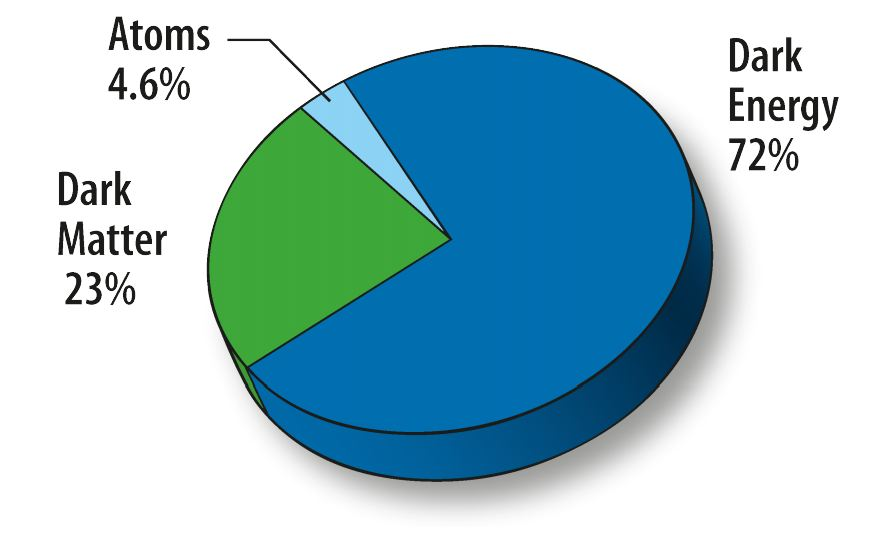
\includegraphics[width = .4\textwidth]{Pie_chart_universe.jpg}
\caption{Constituent percentages for total energy density of the universe, present day. Everyday matter (stars, interstellar gas, etc.) comprises less than 5\% of the total mass-energy density of our universe. Figure from NASA/WMAP science team, 2008 \cite{WMAP}.}
\end{figure}

\section{The $\Lambda$CDM Model of Cosmology}

The $\Lambda$CDM Model is the current generally accepted model for modern cosmology. This model stipulates that the universe is homogeneous and isotropic on its largest distance scales (on the order of gigaparsecs); If we examine the universe temporally, however, we see substantial differences -- we see an evolving universe. In the 1920s, Edwin Hubble showed that the universe is expanding, as evidenced by the redshift of distant galaxies. Hubble demonstrated that our current epoch is seeing an accelerating expansion in the universe.

The conditions of isotropy and homogeneity for this model result in the Friedman-Robertson-Walker (FRW) metric,

\begin{eqnarray}
ds^2 = (cdt)^2 - R^2(t)\left(\frac{dr^2}{1-kr^2} + r^2(d\theta^2 + sin^2(\theta d \phi^2))\right)
\end{eqnarray}

where k identifies spatial curvature (either 0,-1, or +1, which corresponds to flat, negatively-curved, and positively-curved space respectively), and the parameter concerning the evolution of the universe is R(t), the scaling factor, which has dimensions of length. It is worth noting that the Hubble Constant is derived from this scaling factor: $H \equiv \frac{d log R}{dt}$.

The time evolution of this metric, and thus the universe, depends on the contents of our universe. The $\Lambda$CDM model considers three classes of mass-energy: matter, radiation, and the (relatively) recently added dark energy. Each is determined by relative values of energy density $\rho$ and relativistic pressure p. In addition, each scales differently with R(t), the scaling factor:

\begin{enumerate}
\item \textbf{Matter:} non-relativistic material whose energy density decreases as $\sim 1/R^3$ with the expansion of the universe and whose relativistic pressure $\approx 0$. This group includes baryons as well as potential cold dark matter.
\item \textbf{Radiation:} photons and relativistic matter -- such as massless neutrinos -- which have a positive relativistic pressure, and whose energy density decreases as $\sim 1/R^4$ -- faster than matter -- due to redshifts in radiation caused by expansion.
\item \textbf{Dark Energy:} an energy density present in space itself (generally known as vacuum energy) with a negative pressure, and an energy density which does not dilute with expansion of the universe. Proposed cause for the accelerated expansion of the universe.
\end{enumerate}

The inclusion of cold dark matter and dark energy are characteristic features of this cosmological model (as indicated by the name, where $\Lambda$ represents the dark energy cosmological constant, and CDM stands for "cold dark matter").

\subsection{The Density Parameter}

Another feature of the $\Lambda$CDM model is the value of the energy density, $\Omega$. This quantity comes from the Friedmann equations, which govern the expansion of space for the FRW metric. $\Omega$ describes the energy density of our universe, $\rho$, in relation to some critical energy density, $\rho_c$, for which the curvature term in the FRW metric, k, is zero. The density parameter is defined as $\Omega \equiv \rho/\rho_c$.

$\Lambda$CDM cosmology predicts that $\Omega \approx 1$, so that our universe is very nearly flat. This parameter can be separated into the relative contributions of the three classes of energy, defined as $\Omega_{x} \equiv \frac{\rho_{x}}{\rho_{c}}$  such that,
\begin{eqnarray}
\centering
\Omega = \Omega_{m} + \Omega_{r} + \Omega_{\Lambda}
\end{eqnarray}
where $\Omega_{m}$, $\Omega_{r}$, and $\Omega_{\Lambda}$ are the energy densities of matter, radiation, and dark energy respectively. This model predicts that the present energy density is dominated by $\Omega_{m}$ and $\Omega_{\Lambda}$; this arises from their different dispersion relations with the expansion of the universe. $\Omega_{m}$ can be further separated into $\Omega_{mb}$ and $\Omega_{mnb}$ which are the baryonic and non-baryonic contributions.

Experimental observations from three independent sources confirm the dominance of matter and dark energy. These are observations of distant Type 1a Supernovae(SNe), the cosmic microwave background WMAP data (CMB), and observations of baryon acoustic oscillations. Independently, each set constrains the relative energy densities weakly; however, together the data sets provide a consistent set of well-constrained energy density parameters: $\Omega_{mb} = 0.0456 \pm 0.0015$, $\Omega_{mnb} = 0.228 \pm 0.013$, and $\Omega_{\Lambda} = 0.726 \pm 0.015$ \cite{Komatsu2008}. Figure 1.2 shows the constrained parameter space of the $\Omega_{\Lambda}$ - $\Omega_{m}$ plane. Together, they dominate the total mass-energy density of the universe.

\begin{figure}[ht]
\centering
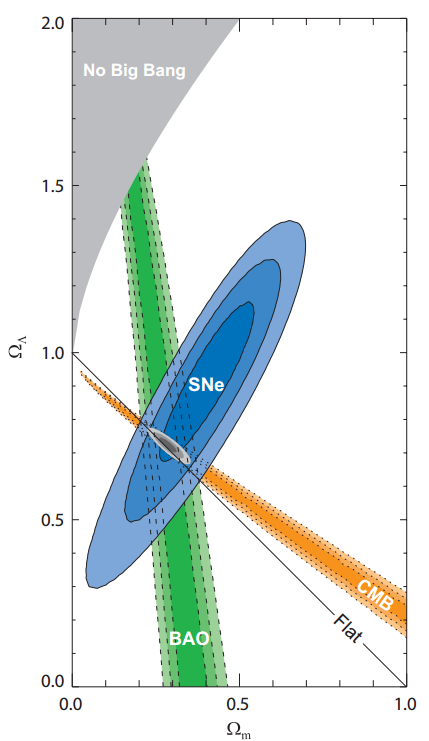
\includegraphics[width = .5\textwidth]{Energy_densities.png}
\caption{Union data for WMAP cosmic microwave background (CMB), baryon acoustic oscillations (BAO), and Type 1a supernovae data (SNe). The shaded areas show 1, 2, and 3$\sigma$ confidence regions. These data provide a consistent region in the energy density parameter space, and seem to indicate a flat universe. Figure from \cite{Kowalski2008}.}
\end{figure}

\subsection{Evolution of the Universe}
The history of our universe, as portrayed by the $\Lambda$CDM model, has some key events which will be of consequence in the sections which follow, therefore are laid out here, chronologically:
\begin{enumerate}
\item The universe originated in the Big Bang, an event which precipitated the current expansion. Before this event, all of space-time was concentrated at $R \approx 0$, in an arbitrarily small, infinitely dense region.
\item Around $10^{-36}$ seconds after the Big Bang, a period of inflation is believed to have occurred, during which the universe expanded by a factor of at least $10^{78}$. This smoothed out initial inhomogeneities, leading to the homogeneous and isotropic universe we currently live in.
\item Approximately 1 minute later, the universe cooled enough to permit fusion of protons and neutrons into the light nuclei (deuterium, helium, and lithium) in a process called Big Bang nucleosynthesis. This process was responsible for the majority of the amounts of these elements present today.
\item Nearly 400,000 years after the Big Bang, cooling had progressed enough for the first neutral atoms to form (hydrogen) from free protons and electrons in a process called recombination. Photons could now travel freely among the neutral atoms, creating a transparent universe. This initial decoupling is the cosmic microwave background we see today.
\item The next few billion years saw the formation of the non-linear structure of the universe due to small inhomogeneities which resulted in gravitational collapse to over-dense regions. Structure formation occurred hierarchically -- with small structures forming first, and large structures forming later.
\item Around 4 billion years ago, the energy density of dark energy overtook that of matter, and the expansion of the universe began to accelerate.
\end{enumerate}

We shall see in the following section that many of these events naturally support the theory of cold dark matter.

\section{Observational Evidence for Dark Matter}

There is significant observational evidence which implies not only the existence of dark matter, but also its likely non-baryonic and non-relativistic nature. Evidence can generally be divided into three main areas: the modern universe, the primordial universe, and structure formation. Evidence in the modern universe includes rotational velocities and velocity dispersions of galaxies and galaxy clusters, strong, weak, and micro gravitational lensing, and intergalactic x-ray emission spectra. The primordial universe provides us with Big Bang nucleosynthesis and the cosmic microwave background, both of which act as "baryometers" setting limits on the amount of baryonic matter in the universe. Finally, the rate of structure formation in the early universe provides further evidence of some form of non-baryonic, non-relativistic, dark matter. These will be discussed in turn below. Even at the time of this writing, techniques continue to improve, our repository of evidence grows, each time adding more support to the current theory of dark matter.

\subsection{Velocity Dispersion in Galaxies and Galactic Clusters}

In 1933, Fritz Zwicky became the first person to use the velocity dispersion within cosmological objects to infer the total mass of the system. His studies of the Coma galaxy cluster led to the conclusion that its actual mass was several hundred times higher than indicated by the amount of radiative matter. He termed this unseen matter \emph{dunkle Materie} or 'dark matter', the first reference to such a material.

The method used by Zwicky is still employed today, with great success, to characterize the mass of galaxies and clusters. For a galaxy, this process calculates the velocities of a large number of constituent stars, finding the velocity dispersion of the group. These velocities are measured through the Doppler shift of characteristic spectra, such as the 21cm HI line. The average kinetic energy can then be related to the gravitational potential through the virial theorem. This method is particularly useful for dwarf and elliptical galaxies, due to their amorphous structure. Clusters (also amorphous) are analyzed in an analogous fashion.

Recent data, particularly from the Sloan Digital Sky Survey (SDSS), has revealed numerous local, faint, dwarf galaxies which have subsequently been analyzed (see Simon and Geha \cite{Simon2007}). Their results reveal a significant dark matter dominance in dwarf galaxies, with mass to light ratios which approach 1000 times the solar mass-to-light ratio ($M_{\bigodot}/L_{\bigodot}$) in some. %explanation?

\subsection{Rotation Curves for Spiral Galaxies}

Analysis of the rotation curves for spiral galaxies also indicates a population of dark matter which -- though not as drastic as in dwarf galaxies -- is still significant. Furthermore, these curves suggest a mass distribution for the dark matter throughout the galaxies. Spiral galaxies present a particularly powerful tool for determining mass distribution, due to the simple near-circular rotational motion of their constituent stars.

A spiral galaxy is structured such that there is a central concentration of stars (the bulge) surrounded by a disc of stars. Given the rotational symmetry of this shape, if the light distribution was indicative of matter distribution, we would expect the rotation velocities -- from basic Newtonian mechanics -- to drop off as $\sim 1/\sqrt{r}$ outside the luminous galactic disk. This has been tested for a multitude of spiral galaxies, with rotational velocities calculated from line-of-sight velocities inferred from Doppler shifts of characteristic spectra: The H$\alpha$ line, the 21cm HI line, CO rotational transition lines, etc. The results, compiled by Sofue and Rubin \cite{Sofue2001}, are shown in Figure 1.3. These curves are drastically different from the behavior expected from a galaxy with most of the mass concentrated toward the center. Instead, the distribution must continue well outside of the luminous disc to allow such high rotational velocities. This is believed to be in the form of some dark matter halo, in which these galaxies are embedded.

\begin{figure}[h]
\centering
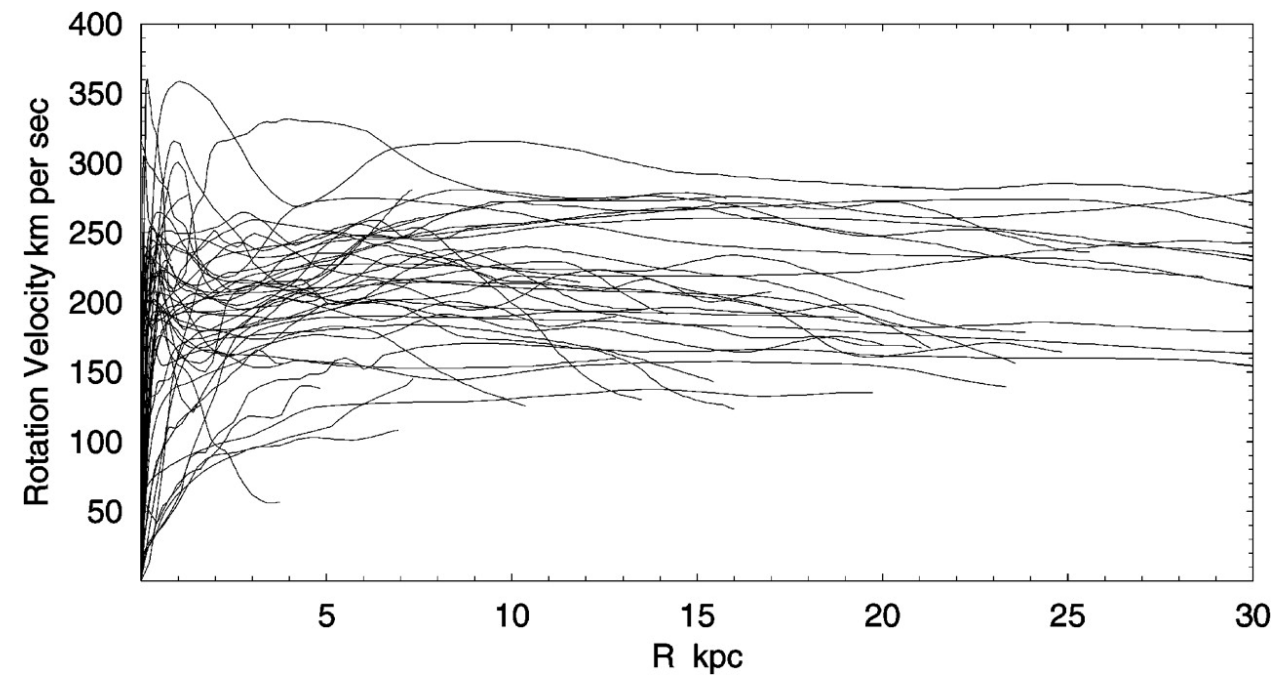
\includegraphics[width = .5\textwidth]{Rotational_velocities.png}
\caption{Aggregation of data on rotational velocities of matter as a function of distance, in kiloparsecs, from the galactic center. The flat rotational velocity curve, as opposed to one which drops off as $\sim 1/\sqrt{r}$ past the central bulge, indicates a mass distribution that extends well past the visible concentration of mass. Figure from \cite{Sofue2001}}
\end{figure}

Various methods have been developed which are able to verify mass values obtained through velocity dispersion in clusters. One such method is observation of x-ray emission spectra from intracluster gas. Intracluster gas is superheated plasma which lies at the center of galactic clusters, and is believed to comprise up to 90\% of the total baryonic matter in a cluster. This gas is heated to temperatures of between $10^7$ and $10^8$ Kelvin by the gravitational energy of the cluster (from collision shockwaves and gravitational potential). At such temperatures, this intracluster medium (ICM) emits x-ray radiation, which can be used to determine the temperature of the ICM. If we assume that the gas is in hydrostatic equilibrium, then given a temperature profile for the ICM, we can infer the total mass of the cluster. Such observations have been made on multiple clusters up to a redshift of $z \approx 0.5$ by the \emph{Chandra} x-ray telescope, which support results obtained through velocity dispersion \cite{Vikhlinin2005,Vikhlinin2009}.

\subsection{Gravitational Lensing}

General relativity predicts that the path of light will be bent in the presence of a gravitational potential. Einstein first observed this phenomenon as the bending of starlight passing near the sun during a total solar eclipse. The same phenomenon occurs at the intergalactic scale, with the gravitational potential of the sun replaced by that of a galaxy or a cluster. This gravitational potential acts as a lens with an effective refractive index,

\begin{eqnarray}
n(x) = 1 + \frac{2}{c^2}|\Phi(x)|
\end{eqnarray}

so characterizing the path of the light allows us to determine the potential, and thus the mass of the lensing object. Figure 1.4 shows a diagram of the process of gravitational lensing.

\begin{figure}[h]
\centering
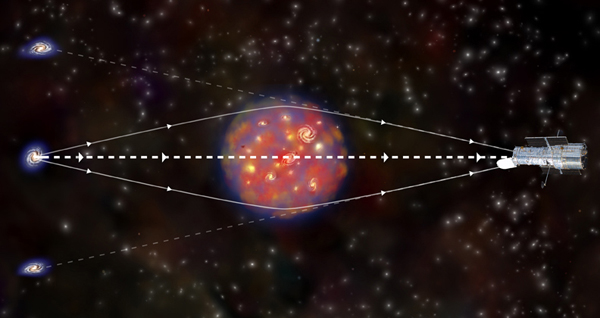
\includegraphics[width = .4\textwidth]{Lens_diagram.jpg}
\caption{Representation of the process of gravitational lensing. Light from the distant blue galaxy is refracted from the central cluster. This creates multiple images of the galaxy as shown by the faint dotted lines. Image from the Chandra X-ray Observatory website \cite{lens}.}
\end{figure}

There are three general groups of gravitational lensing:

\begin{enumerate}
\item \textbf{Strong Lensing:} Occurs when the mass density of the lensing object is high enough to produce visible distortion of background objects in the form of arcs or full Einstein rings. Requires near-direct alignment of observer, lensing object, and background source.
\item \textbf{Weak Lensing:} Smaller-effect lensing where the distortion of background objects must be inferred from statistical correlations among the visible shapes. Doing so allows the mass distribution of the lensing object to be determined. Far more common than strong lensing phenomena.
\item \textbf{Microlensing:} Effect caused by lensing objects of much smaller mass, such as a planet or star. Not strong enough to cause detectable distortion, but can be observed through a variation in background object brightness with the increase, peak, then decrease of the lensing effect as the lensing object moves in front of the background object.
\end{enumerate}

Strong lensing and weak lensing are of particular importance in the theory of dark matter. They allow us to infer the total mass as well as its distribution throughout a gravitational lens. Studies of strong lensing from clusters such as Abell 2218 have led to the conclusion that there is simply not enough luminous matter to reproduce the lensing observed. Estimates for the mass-to-light ratio Abell 2218 range from 80 to 180 depending on the part of the cluster under observation, strongly supporting the presence of significant dark matter \cite{Kneib1995,Kneib1996}.

Weak lensing studies, though more difficult, have been pursued by collaborations \cite{Sheldon2009} on more than 130,000 galaxy clusters and groups. Their mass results generally agree with those obtained for the velocity dispersion methods. Furthermore, the large structure of clusters allows us to treat their properties as representative of the larger universe; by measuring $\Omega_{m}$ for these clusters, we are essentially determining $\Omega_{m}$ for the universe as a whole. Results from these studies have confirmed -- completely independently -- the value of $\Omega_{m} \approx 0.2 - 0.3$, providing support for the $\Lambda$CDM model \cite{Sheldon2009}.

\begin{figure}
    \centering
    \subfloat[]{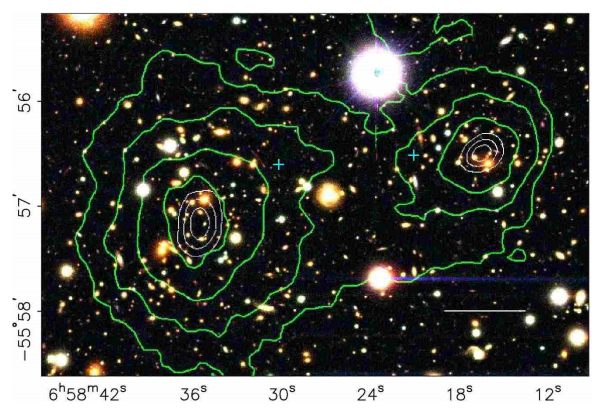
\includegraphics[width=.3\textwidth]{Bullet_visible.png}}
    \subfloat[]{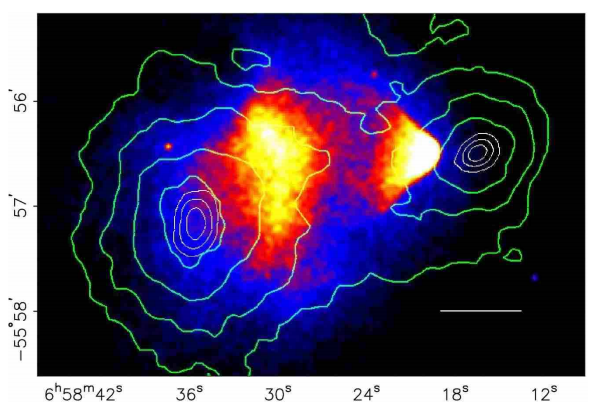
\includegraphics[width=.3\textwidth]{Bullet_xray.png}}
    \caption{Images of the Bullet Cluster, which show a clear discrepancy between the location of the baryonic matter (imaged by X-rays) and the total mass distribution. Both the visible light image (a) and the X-ray image (b) are superimposed on the mass contours inferred from weak lensing.}
\end{figure}

One of the most compelling subjects for weak lensing studies at the moment is the Bullet Cluster (1E057-558). The Bullet Cluster is actually two clusters, visible just after collision. Clowe and coauthors have analyzed the weak lensing phenomenon -- thereby constructing the mass distribution -- and compared it to the ICM distribution (which contains the majority of the baryonic matter in a cluster). The results, shown in Figure 1.5, display a substantial contrast in the distribution of the ICM and the mass contours inferred from weak lensing. We see that the majority of the clusters' mass has continued moving unperturbed -- it did not undergo collision. These observations indicate that the majority of the clusters' mass is not only dark, but also must have a very small collision cross-section (i.e. it is non-baryonic).

\subsection{Big Bang Nucleosynthesis}

$\Lambda$CDM cosmology predicts that a period of intense nucleosynthesis occurred from roughly three minutes to twenty minutes after the Big Bang, after the universe had cooled enough to allow fusion, which created the light nuclei: deuterium ($^2H$), helium ($^3He,^4He$), and lithium ($^7Li$). The relative abundance of each of these elements depended solely on three factors: the baryon mass density, the expansion rate of universe, and the neutron-proton ratio. The last factor, neutron-proton ratio, can be determined assuming that weak interactions at this time were in thermal equilibrium. With this, the neutron-proton number densities are $n/p = e^{-Q/T}$, where Q is the neutron-proton mass difference, and T is temperature \cite{Amsler2008}. These first two factors, baryon mass density and expansion rate, can be reduced to a dependence on the ratio of baryons to photons: $\eta \equiv \eta_{b}/\eta_{\gamma}$ (photon density governs expansion rate). Photon density, however, can be determined from the temperature of the cosmic microwave background. Therefore, measuring the relic abundance of the light elements gives an accurate measurement of baryon density.

Deuterium is the most accurate "baryometer" of these light elements for two reasons. First, deuterium levels have a strong dependence on $\eta$, as shown in Figure 1.6 (note that the axes are logarithmic). Second, no galactic processes are currently known to exist which can produce significant amounts of deuterium. Measuring abundances of deuterium (which have not been disturbed by galactic evolution processes which can destroy deuterium) can therefore accurately determine relic deuterium abundances. Such candidates are low-metallicity stars (Population II and Population III) and low-metallicity primordial gas (ICM dubbed Lyman-$\alpha$ forests). Recent measurements of deuterium were conducted using absorption lines from high z ($\approx 3$) quasars illuminating intermediary metal-poor Lyman-$\alpha$ forests. These measurements give $\langle log(^2H/H)_{p} \rangle = -4.55 \pm 0.03$ and $\Omega_{b,0}h^2 = 0.0213 \pm 0.0010$ (68\% confidence limits) where the subscript $p$ denotes primordial abundance and $(^2H/H)$ is abundance relative to elemental hydrogen \cite{Pettini2008}. The $\Omega_{b,0}h^2$ represents the current baryonic matter portion of the critical density. The agreement between these numbers, and those found from the CMB power spectrum are shown in Figure 1.6. Their concordance lends strength to the belief that any significant presence of dark matter must be non-baryonic in nature.

The other light elements have also been used to calculate $\eta$, but due to difficulties in detection, as well as problems with post-BBN creation of these elements, results vary (see Figure 1.6). Specifically, the origin of the large discrepancy between the observed abundance of $^7Li$ and the predicted abundance is a source of debate (see \cite{Amsler2008}). Though models (or theories) still need to be adjusted to encompass $^7Li$, Big Bang nucleosynthesis provides strong evidence for the presence of a significant amount of non-baryonic dark matter.

\begin{SCfigure}[.7][h]
\centering
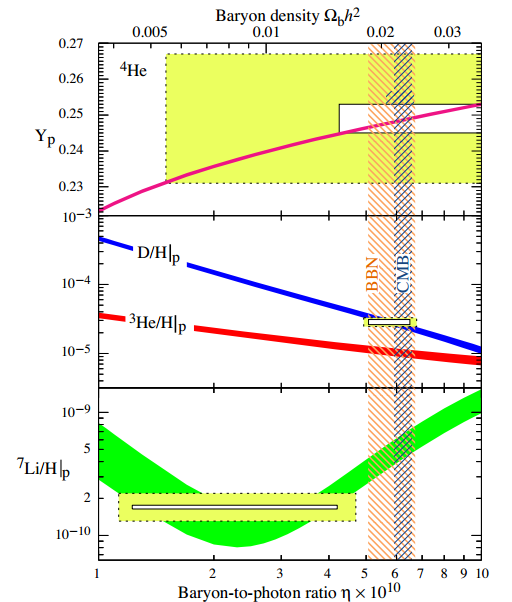
\includegraphics[width = .4\textwidth]{Deuterium.png}
\caption{Comparison of light element abundances from various sources. Curves show abundances as predicted by the standard model of Big Bang nucleosynthesis \cite{Cyburt2008} (95\% CL). The hatched vertical regions show predictions of baryon density from BBN and measurements of the CMB (also 95\% CL). The boxes show the actual observed abundances of these light elements and their agreement (or disagreement in the case of $^7Li$) with predictions;the inner boxes represent $\pm2\sigma$ statistical error, while the outer boxes are statistical and systematic errors. Figure from \cite{Amsler2008}.}
\end{SCfigure}

\begin{SCfigure}[.7][h]
\centering
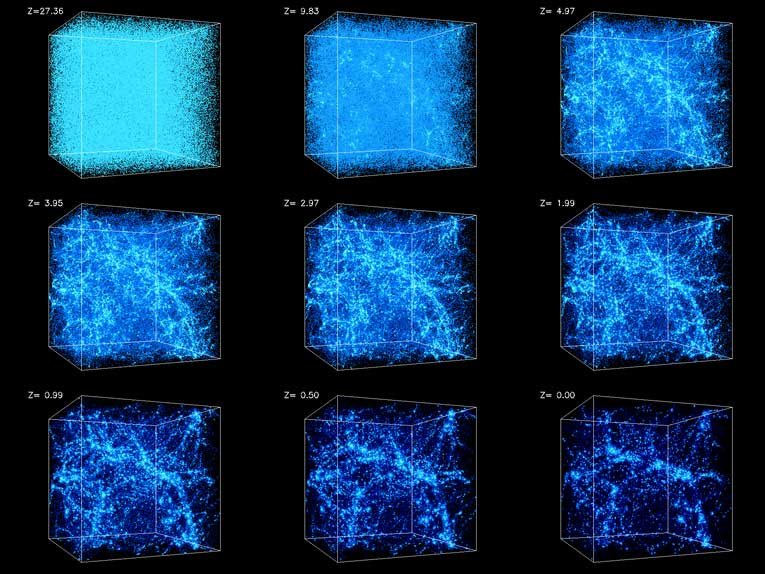
\includegraphics[width = .5\textwidth]{structure_formation.jpg}
\caption{Numerical simulations of the formation of structure in the universe from z=30 to the present over a box 43MPc in size. We see how the nearly homogeneous early universe aggregates into the overdensities to form the structure of superclusters we see today. Notice that by around z = 1, most of the structure has formed and begins to separate. Past this period dark energy dominates, which prevents further large-scale formation of structure. Figure from \cite{Simulation}.}
\end{SCfigure}

\subsection{Universal Structure}
Observations of the Cosmic Microwave Background (CMB) and other early large-scale structures present us with another set of primordial evidence which indicates significant dark matter abundance, suggests its non-baryonic nature, and requires it to be "cold" (i.e., non-relativistic at the time of the early universe).

\subsubsection{Anisotropies in the CMB}
The cosmic microwave background is an image of the early universe just after recombination. Once neutral atoms were formed, photons were decoupled from baryonic matter, and propagated through the universe. This period is called the drag epoch. The 2.73K black body radiation forming the CMB is a result of these first photons. Once photons were decoupled from baryons, baryonic matter could begin to clump into the slight matter over-densities, and begin to form large-scale structures. This process is modeled in $\Lambda$CDM by linear perturbation theory for early epochs, and numerical simulations for later periods using a relativistic theory of gravitational collapse (see \cite{Kolb1990}, \cite{Padmanabhan1993}, \cite{Liddle2000} for an explanation of the theory). Figure 1.7 shows one such numerical simulation.

By observing the temperature anisotropies in the CMB signal (which gives photon anisotropy) we can determine baryon anisotropies at the time of the drag epoch. This is due to the tight coupling of baryons and photons prior this epoch. These anisotropies are defined by over-densities and under-densities in the energy field,

\begin{eqnarray}
\delta(\vec{x},t) \equiv \frac{\rho(\vec{x},t) - \langle\rho(t)\rangle}{\langle\rho(t)\rangle} \\
\delta(\vec{k},t) \equiv \frac{1}{(2\pi)^{3/2}} \int \delta(\vec{x},t) e^{-\vec{k} \cdot \vec{x}} d^3 \vec{x}
\end{eqnarray}

where $\bar{\rho}(t)$ is the mean energy density of the universe at time t, and $\delta(\vec{k},t)$ the statistical distribution of the density variation for different length scales. The theory of gravitational collapse modeling the formation of structure requires these anisotropies be $\geq 10^{-3}$ at the time of recombination to allow the creation of bright galaxies as far back as $z \approx 7.6 $ \cite{Bradley2008} and the superstructures we see today. However, baryon anisotropies at similar length scales in the CMB are only observed to be $\approx 10^{-5}$. Such small anisotropies could not have formed the structures we see in similar time scales.

Dark matter provides a solution to this problem if we stipulate the existence of some \emph{non-baryonic} dark matter, as espoused by Big Bang nucleosynthesis models. This non-baryonic dark matter did not interact electromagnetically, therefore felt none of the effects of scattering photons. As a result, dark matter was able to settle into over-densities, creating gravitational potential wells long before recombination. After photon decoupling, baryons could then gravitate toward these pre-established potential wells more quickly, forming the baryon structure we see today.

\begin{SCfigure}[.7][h]
\centering
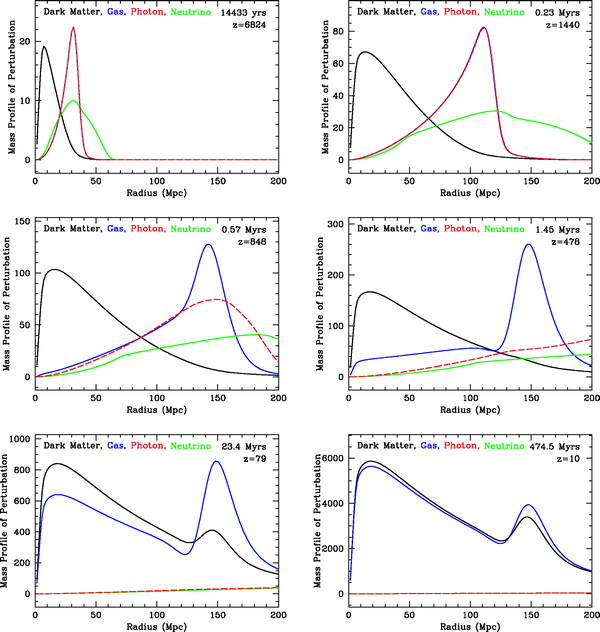
\includegraphics[width=.4\textwidth]{BAO_propagation.jpg}
\caption{Formation of baryon acoustic oscillations. Perturbations in energy density of the early universe created sound waves in the photon-baryon plasma. These waves propagated outward with photons and baryons coupled until the drag epoch freed photons and left the baryon peak stalled. This baryon peak remained as a feature in the density correlation function at $\approx 150$ MPc. Figure from \cite{Eisenstein2007}. }
\end{SCfigure}

Solving the problem of structure formation with the addition of dark matter sets another constraint on the properties any dominant dark matter candidate: it must be non-relativistic by early epochs ($z > 1000$). Relativistic matter would not have created the large potential wells required, and would not have resulted the baryon acoustic oscillations described below. Relativistic matter would have resulted in "top-down" formation of structure, where the largest structures form first. This is opposite of the hierarchical formation posited by the $\Lambda$CDM model, and does not match with observations and simulations.


\subsubsection{Baryon Acoustic Oscillations}

The argument for non-baryonic dark matter of further supported by the recent identification of baryon acoustic oscillations in large-scale structure by the Sloan Digital Sky Survey (SDSS), the 2dF Galaxy Redshift Survey (2dFGRS), and the five-year Wilkinson Microwave Anisotropy Probe (WMAP). These signatures, present in both the CMB ($z \approx 1000$) and strucures at low redshift (low z), provide powerful tools to constrain $\Omega_{m}$, $\Omega_{b}$, and $\Omega_{\Lambda}$, and offer further confirmation of $\Lambda$CDM cosmology.

Baryon acoustic oscillations, first predicted in 1970, are acoustic waves in baryonic matter which were formed in the early universe before the drag epoch. We can see the imprint left by these waves in the structure of our universe. The process (shown in Figure 1.8) is as follows \cite{Eisenstein2005}:

\begin{enumerate}
\item Over-dense dark matter regions attracted baryonic matter, while photon pressure drove baryonic matter outward (dark matter, which does not interact electromagnetically, was unaffected). This perturbation excited sound waves in the photon-baryon plasma.
\item This acoustic wave traveled outward at nearly half the speed of light (the speed of sound in the plasma) with the photon and baryon peaks coupled.
\item Once the universe cooled enough through expansion, photons and baryons decoupled in the drag epoch. This drastically reduced the speed of sound. Photons streamed outward at the speed of light, while the baryons -- losing their driving pressure -- stalled.
\item The dark matter perturbation drew baryons back toward the center, while the baryon perturbation drew dark matter outward. This spread the matter distribution. A peak in baryon distribution remained at the radius of the sound horizon (the baryon peak at the time of decoupling).
\item The dark matter and baryon perturbations seeded formation of structure in the universe, resulting in a density correlation peak at a co-moving radius of around 150 MPc.
\end{enumerate}

Detecting the signal of these BAO is impossible without statistical analysis, as the myriad over-densities in the early universe meant creation of many interfering oscillations, which would just appear as turbulence. However, by statistical correlation measurements of over-densities, these features can be distinguished. Analysis from the five-year WMAP survey has successfully measured these oscillations as fluctuations in the power spectrum of the cosmic microwave background, placing the \emph{co-moving} sound horizon at $\sim 150$ MPc \cite{Komatsu2008}.

Whether these oscillations would still be visible in the modern universe depends on how expansion proceeded after their formation. Predictions from $\Lambda$CDM cosmology stipulate that early expansion provided linear perturbation growth. This type of growth leaves the Fourier components of the waves uncoupled, preserving well-defined features such as the sound horizon \cite{Eisenstein2005}. These features should then leave a detectable imprint on the structure of the modern universe. The Sloan Digital Sky Survey and the 2dF Galaxy Redshift Survey are the first experiments to be able to detect these faint signatures in modern matter densities. The results from the LRG (luminous red galaxy) data set in SDSS are shown in Figure 1.9. This plot shows a two-point correlation function calculated for $\sim$ 46,000 galaxies at a redshift $0.16 < z < 0.47$. The sound horizon is clearly visible at a co-moving distance of roughly 150 MPc.

\begin{figure}[h]
\centering
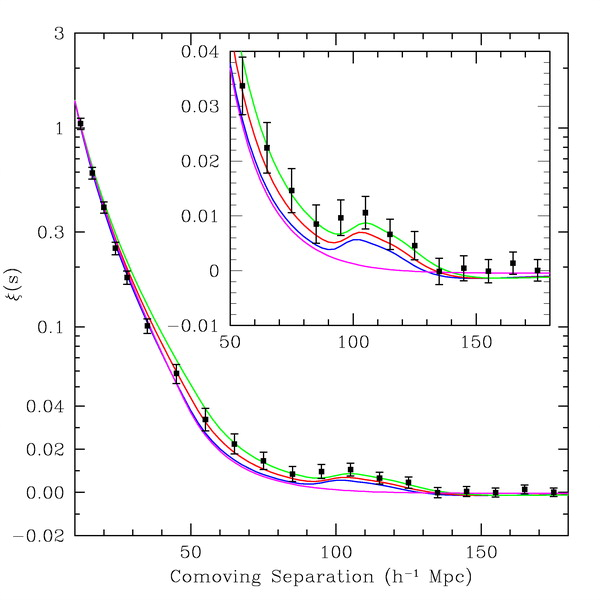
\includegraphics[width = .5\textwidth]{BAO_peak.jpg}
\caption{Correlation function found from Sloan Digital Sky Survey, LRG sample. The sound horizon, emphasized in the magnified box, is observed at $\sim 100 h^{-1} MPc$ (150 MPc). The colored lines show various cosmological parameter models: green shows $\Omega_{m}h^2 = 0.12$, red shows $\Omega_{m}h^2 = 0.13$, blue shows $\Omega_{m}h^2 = 0.14$. All assume that $\Omega_{mb}h^2 = 0.024$. The bottom pink line shows a purely dark matter curve ($\Omega_{m}h^2 = 0.105$), which lacks the peak entirely. Figure from \cite{Eisenstein2005}.}
\end{figure}

The presence and characteristics of BAO provide a wealth of information about the structure and evolution of the universe. First, the simple presence of BAO in the promordial and modern universe evidences the linear perturbation growth predicted by $\Lambda$CDM cosmology. Second, the shape of the peak provides information on $\Omega_{\Lambda}$, $\Omega_{m}$, and $\Omega_{mb}$ (baryonic matter density). The smallness of the peak in Figure 1.9 suggests a dominance of dark matter over baryonic matter, but also predicts that $\Omega_{m}h^2 \approx 0.12$ -- based on the best fit described in the figure -- leading to a dominance of dark energy in the modern universe. Third, by confirming the size of BAO at z $\sim$ 1000 and z $\approx .16$ we create a standard length scale which can tell us about the expansion of the universe, independent of supernova observations. Though the data is not accurate enough to do so at the moment, future measurements of BAO could provide a method to independently determine the Hubble parameter (H(z)) \cite{Eisenstein2005}.

Full data for WMAP, SDSS, and 2dFRGS surveys, combined with observations of distant Type 1a Supernovae create the plot shown in Figure 1.2 and described in section 1.2.1. Baryon acoustic oscillations play an important role in this figure, as they provide independent measures of the cosmological parameters. Their agreement with cosmic microwave background and supernova data provides strong support for the $\Lambda$CDM model of cosmology.

\section{Candidates for Dark Matter}

The large body of evidence which supports the existence of dark matter has allowed us to infer many of its properties. The dominant dark matter in our universe must be non-baryonic, non-relativistic ("cold"), stable enough to have a lifetime which is large compared to the age of the universe, and must be nearly non-interacting. Though we have constrained many of its properties, we still must ask: \emph{what is it?}. As of this writing, this question is still unanswered, but its properties inferred from the body of indirect evidence drastically narrows the list of likely candidates. I will discuss one of the most promising members of this list, Weakly Interacting Massive Particles or WIMPs.

\subsection{WIMPs}

WIMPs (Weakly Interacting Massive Particles) are a hypothetical class of particles which interact with other matter only through weak-scale processes ("weakly interacting") and gravity. They have a hypothesized mass of $10GeV \leq M \leq 10TeV$ ("massive"). WIMPs are a favored candidate for dark matter (and the subject of our collaboration's scrutiny) not only because they would satisfy the constraints described above, but also due to cosmological considerations which predict weak-scale interaction cross-sections for dark matter particles caused by a process called "freeze out".

\begin{figure}[h]
\centering
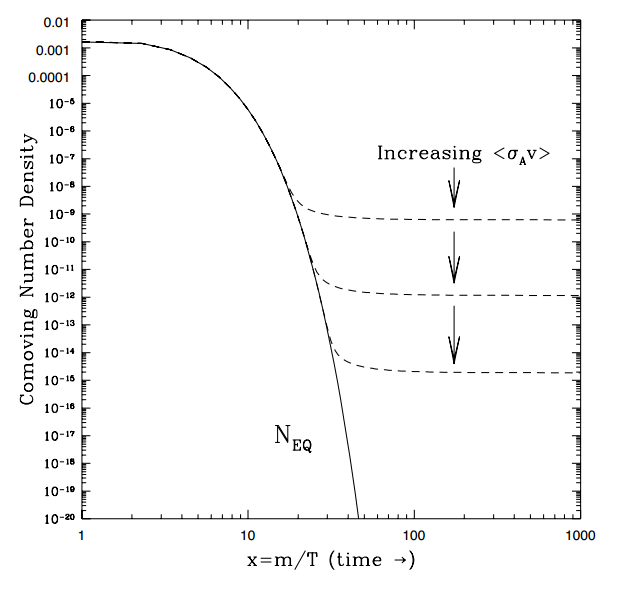
\includegraphics[width = .4\textwidth]{annihilation_crosssection.png}
\caption{Figure showing the co-moving number density of of particle as a function of temperature. The solid line represents the period in which the particle is in thermal equilibrium; the dashed curve represents relic abundances as a function of annihilation cross-section. Larger annihilation cross-sections result in lower relic densities. Figure from \cite{Kolb1990}.}
\end{figure}

The full argument for the cosmological constraints on interaction cross-sections for dark matter particles is beyond the scope of this chapter, but the main argument will be reviewed here. First, the abundance of a particle in the modern universe is determined by its creation and annihilation rate throughout the evolution of the universe. Figure 1.10 shows the process for determining the co-moving number density of a hypothetical particle. A particle in the early universe (just after the inflationary epoch) would be in thermal and chemical equilibrium with the primordial plasma, such that its creation from thermal production and annihilation rate were equal. The annihilation rate is given by $\Gamma$, where
\begin{eqnarray}
\Gamma = n\langle \sigma v \rangle ,
\end{eqnarray}

and $n$ is the number density of the particle, $\sigma$ is the annihilation cross-section, $v$ is the relative velocity of the two particles, and the brackets denote an average over the thermal ensemble. This rate will be equal to thermal production as long as $T >> m$, where $m$ is the mass of the particle. The number density would be constant. As T drops, thermal production stops and the number density for a massive, non-relativistic particle in thermal equilibrium after this point would be proportional to the Boltzmann constant, $n \propto e^{-\frac{mc^2}{k_bT}}$. This is shown as the solid curve in Figure 1.10. The particle would remain in thermal equilibrium until annihilation becomes inefficient, below $\Gamma \sim H$. This is known as "freeze out". The relic density after this transition is approximately \cite{Jungman1996},

\begin{eqnarray}
\Omega h^2 \approx \frac{0.1pb \cdot c}{\langle \sigma v \rangle} .
\end{eqnarray}

where c is the speed of light, and pb refers to a picobarn. This can be understood generally as follows: a particle with a larger cross-section will stay in thermal equilibrium for slightly longer, resulting in a exponential suppression in the number density from the Boltzmann factor. Figure 1.10 shows expected co-moving relic densities for increasing cross-sections. From equation 1.7, to obtain relic density near that expected for dark matter ($\Omega h^2 \sim 0.1$) would require a cross section characteristic of the weak scale. Such a particle would have a mass, $m \sim 100 $ GeV.

Particle physics offers further motivation for the existence of a new particle at the weak scale. This motivation, completely independent from cosmological motivations, comes from efforts to address the "hierarchy problem" in the Standard Model (see \cite{Filippini2008} for the argument). Theories which address this problem typically call for the existence of a new particle at the weak scale. Thus, there exists strong motivation for a weakly interacting dark matter candidate. When coupled with the theoretical possibility for detection of such a particle, the allure of WIMPs as the favored dark matter candidate becomes obvious.

\section{The Cryogenic Dark Matter Search and Direct Detection}

Direct detection is the ultimate goal in determining any dark matter candidate. Indirect evidence provides us with clues as to the properties of candidates and motivates their existence, but only direct detection will allow us to confirm the existence of and fully characterize a candidate. Currently, there are roughly two dozen experiments worldwide which have engaged in the search for direct dark matter detection. These experiments use a variety of techniques in an effort for dark matter detection (see Figure 1.11).Our collaboration, CDMS, is one of the leading groups in the direct detection efforts. This section will explain the general principles governing our experiment as well give a brief history of its evolution since inception.

\begin{figure}[h]
\centering
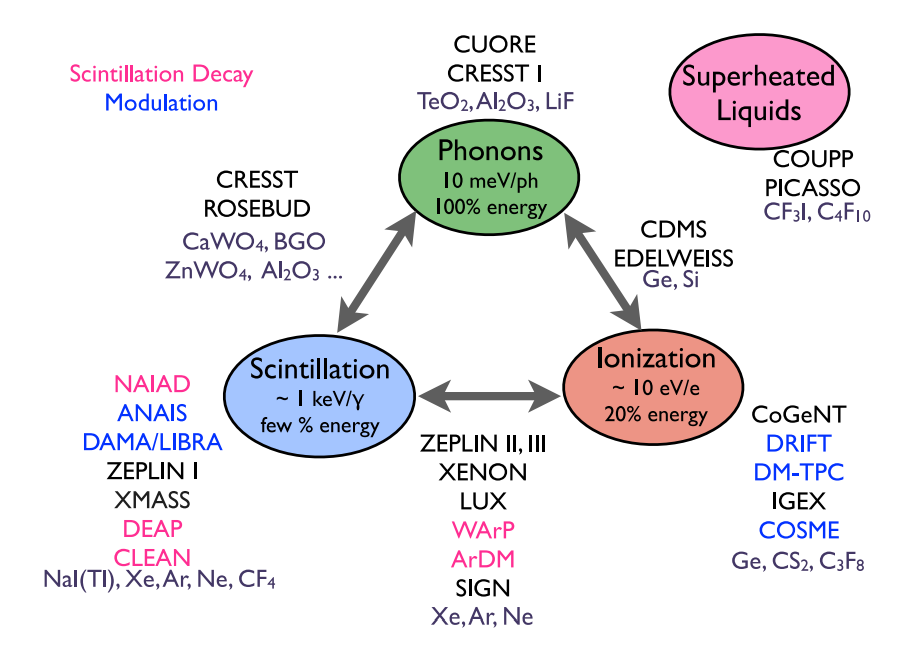
\includegraphics[width = .5\textwidth]{Dm_experiments.png}
\caption{Different detection methods utilized by dark matter experiments. The CDMS Experiment uses phonons and ionization for improved background rejection. Figure from \cite{Figueroa2011}.}
\end{figure}

The CDMS Experiment has been taking data in low background environments since 1996. In the years since then, the experiment has gone through several iterations: CDMS I, CDMS II, SuperCDMS Soudan, and SuperCDMS SNOLab (currently under development). Detection technology has changed significantly, but the basic principle remains the same: that WIMPs will scatter elastically off nuclei in atoms, producing a signal which can be detected as energy deposition. This energy deposition can be characterized through the collection of phonons and charge from interaction recoils. Characterizing each "event" (nuclear or electron recoil in the detector) allows us to discriminate possible WIMP interactions from background.

\subsection{Background}

For our experiment, background is anything that could be misconstrued as a WIMP interaction. The major background in our experiment consists of $\beta$, $\alpha$, $\gamma$ radiation, as well as neutrons and cosmic ray muons. These background events can occur at a rate of $ \sim 10^{13}$ times that for predicted WIMP events, therefore extensive measures are taken to reduce their occurance.

The experiment uses multiple stages of shielding to drastically lower this background:
\begin{enumerate}
\item \textbf{Underground:} experiment location determines muon flux. CDMS I was located at the Stanford Underground Facility (SUF) which provided shielding of 16 meters water equivalent (mwe). This reduced the observed muon flux by a factor of 5 \cite{Abusaidi2000}. CDMS II moved to the Soudan mine in Minnesota which provides $\sim 2100$ mwe. SuperCDMS SNOLab will move to the SNOLab facility (at the Sudbury mine in Ontario Canada) which provides $\sim 6000$ mwe shielding. These depths greatly reduce muon flux as well as cosmic ray gammas (a factor of $\sim 1000$ from Soudan to SNOLab facility \cite{Saab2012}.
\item \textbf{Active veto:} To further mitigate the muon background, a muon scintillator surrounds the experiment. This detects muons and can rule out muon coincident events in the detector (rendered unnecessary in SNOLab).
\item \textbf{Polyethylene:} A circular shield of polyethylene is placed inside the active veto to moderate neutrons produced by muons interacting with the active veto.
\item \textbf{Lead:} 23cm of lead shields the experiment from external gammas.
\item \textbf{Ancient Lead:} A layer of low activity lead (obtained from a Roman shipwreck) shields betas from the outer lead.
\item \textbf{Polyethylene:} A final layer of polyethylene shields the experiment from the ancient lead.
\item \textbf{Radiopure Experiment:} Finally, all of the materials used inside of the dilution fridge containing the experiment are selected for extreme radiopurity to prevent \emph{production} of any background in the experiment. In addition, care must be taken to prevent activation of any materials from cosmic rays.
\end{enumerate}

After these extensive measures are taken to minimize background, we are still left with $\sim 1$ event/kg/KeV/day \cite{Saab2012}. Methods must then be developed to distinguish these background events from possible WIMP signals, as discussed below.

\subsection{Basic Detection Method}

The detection methods used in the CDMS experiment are phonon and ionization signals. These methods use an ultra-pure (as low as $10^{13}$ impurities/$cm^3$) single-crystal semiconductor material such as Germanium or Silicon cooled to $\sim 20$ mK in a dilution fridge. These extreme temperatures are necessary to limit thermal noise present and thus increase sensitivity to particle collisions with the detector lattice. When a particle collides with the lattice, two things happen:
\begin{itemize}
\item Free electron/hole pairs are created due to the semiconductor nature of the detector. These charges can be collected by applying a voltage across the detector.
\item Athermal phonons are excited in the lattice, which can be detected through various means.
\end{itemize}

These two methods of detection provide a powerful tool for discerning between possible WIMP interactions and background events which penetrate to the detector. This is because most background particles interact with atomic electrons (electron recoil). Only neutrons and WIMPs interact with the nucleus of an atom (nuclear recoil). These recoils deposit energy through ionization and phonon production differently. These differences can be described by the ionization yield, Y, which is the ratio of energy deposited through ionization to the amount deposited as phonons. Electron recoil typically has Y$\sim$1 while nuclear recoil has a Y$\sim$0.3. Since background is heavily dominated by electron recoil interactions, this method is very useful for background rejection.

We present a brief description of each generation of the CDMS experiment -- highlighting technological improvements -- below.

\subsection{CDMS Soudan Tower Design}

\subsubsection{CDMS I}
The first experiment used two detector types: BLIP (Berkeley Large Ionization- and Phonon-based) and FLIP (Fast Large Ionization- and Phonon-based) detectors. BLIPs used neutron transmutation doped Ge thermistors (NTD) bonded to Ge crystals. These collected phonon energy through a calorimetric temperature change in the crystal. FLIPs, on the other hand, used W QETs for phonon collection. BLIPs were germanium detectors, while FLIPs were either germanium or silicon. Germanium was ultimately adopted in later experiments due to the larger nucleus which improved probability of nuclear recoil for heavier WIMPs. Both technologies used JFET ionization sensors on one side which received charges through a voltage established across the bulk of the detectors.

\textbf{W QETS:} W QETs (Tungsten Quasiparticle-trap-assisted Electro-thermal-feedback Transition-edge-sensors) use aluminum pads lithographically patterned on one surface of the detectors with an array of tungsten wires attached to them. The tungsten wire is held near its superconducting transition temperature ($\sim$ 80 mK). The superconducting aluminum pads cause phonons to deposit energy as heat. This heat causes an abrupt transition in the tungsten, whose change in resistivity is detected as a current pulse in a SQUID amplification array. This method allowed for a factor of 10 better sensitivity in phonon detection, as well as X-Y localization of the event to within a few millimeters \cite{Gaitskell1997}.


\begin{figure}[h]
\begin{centering}
\subfloat[Left side shows four phonon channels, while right shows two charge channels.]
  {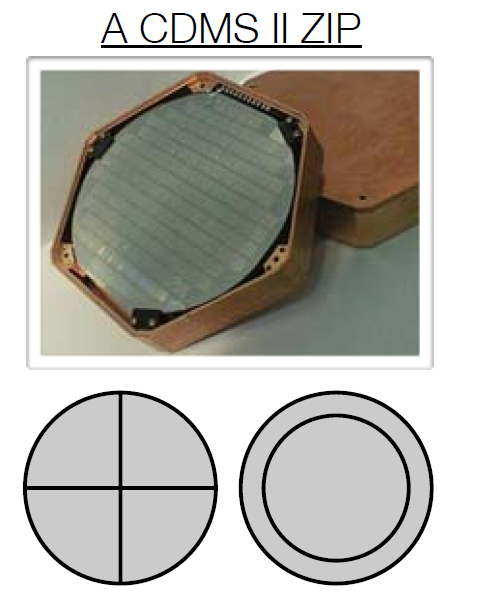
\includegraphics[width=0.3\textwidth]{ZIP.png}}
  \hspace{10pt}
  \subfloat[iZIP detectors have four phonon channels and two charge channels on each side.]
  {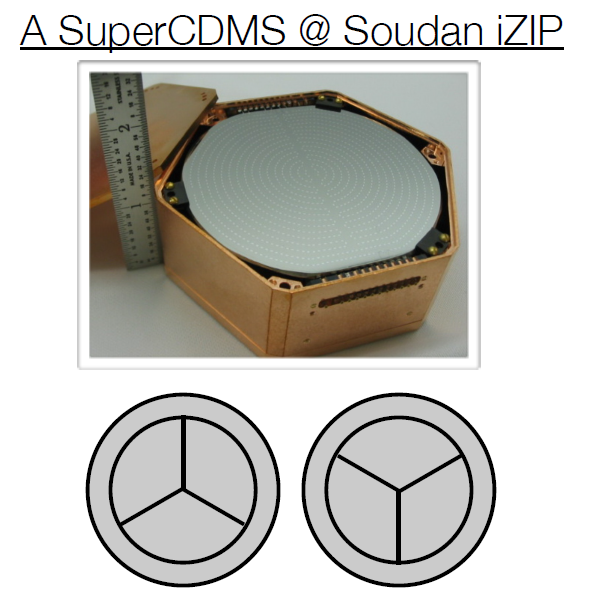
\includegraphics[width=0.3\textwidth]{iZIP.png}}
  \subfloat[SNOLAB detectors will have six phonon channels and two charge channels on each side.]
  {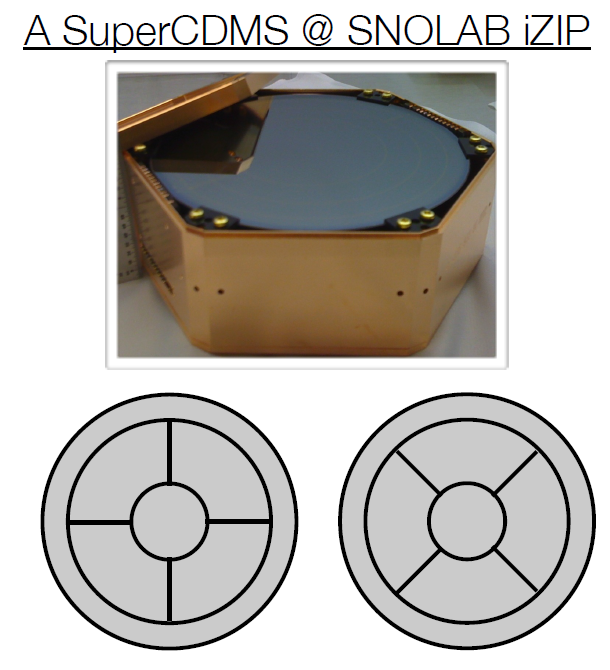
\includegraphics[width=0.3\textwidth]{iZIP_snolab.png}}
\caption{Detector layout for CDMS experiments. Pictures from \cite{Saab2012}.}
\end{centering}
\end{figure}

\subsubsection{CDMS II}

CDMS II was located in the Soudan mine, which drastically reduced cosmic ray background. This is important, especially for muon flux, as muons can produce neutrons in materials. This neutron background is significantly more difficult to distinguish from possible WIMP interactions than other types of background, as it produces nuclear recoil rather than electron recoil. Another major improvement was the development of ZIP (Z-sensitive Ionization- and Phonon-based) detectors. ZIPs had four phonon channels on one side and two charge collection channels on the other side of the detector. Figure 1.12 a) shows the layout of the phonon and charge channels for the ZIP detectors. These detectors built upon the FLIP technology in CDMS, and by creating four phonon channels allowed further localization of events. Combined with ionization yield, this increased electron recoil rejection to $> 10^{-6}$ (only 1 in $10^6$ electron recoil events would be mistaken for a WIMP signal) \cite{Saab2012}.

\subsubsection{SuperCDMS Soudan}

The next generation of the experiment greatly improved detector technology with iZIPs -- where the "i" stands for interleaved. This germanium detector has four phonon channels and 2 charge channels on \emph{each side} as can be seen in Figure 1.12 b. The layout not only provides localization improvements (e.g. unambiguous radial positioning of events \cite{DOE}) but also addresses the largest source of background for the CDMS II experiment: leakage events \cite{Akerib2005}.

\begin{figure}[h]
\centering
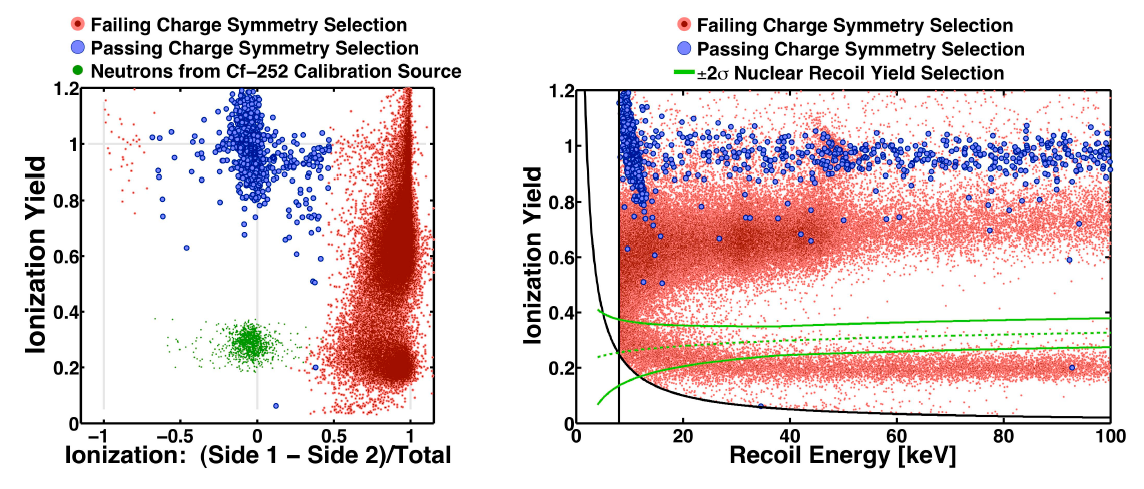
\includegraphics[width = .8\textwidth]{iZIP_ionization.png}
\caption{Utilization of iZIP symmetry conditions to reject surface "leakage" events. These events occur close enough to the surface so that charge is only collected on one side, breaking symmetric charge collection.}
\end{figure}

\textbf{Leakage Events:} These leakage events are electron recoil interactions which occur in the "dead zone" of the detectors (near the surface) where charge collection efficiency is lower. This produces low ionization yields which "leak" into the nuclear recoil regime of the signal, as shown in Figure 1.13 on the right plot. The lowest electron recoils overlap with the nuclear recoil regime, where they can be mistaken for nuclear recoils. By locating charge channels on both sides and establishing a voltage difference between charge and phonon channels, an electric field is produces such that electron recoils that occur within $\sim$ 1 mm of the surface are only collected on one side. This distinguishes the low ionization electron recoils from symmetric charge collection nuclear recoils. Symmetry selection now allows us to rule these events out with a rejection of $10^{-5}$ \cite{Saab2012}.

\subsection{SuperCDMS SNOLab}

The next generation CDMS experiment will take place in the Sudbury mine in Ontario, Canada. This mine is nearly three times as deep as Soudan, which will render the muon flux negligible. Furthermore, the design of the detector will change once more so that it is larger, with six phonon channels and two charge channels on each side, as seen in Figure 1.12 c), which leads to a further increase in signal sensitivity and improves rejection of backgrounds. Additionally, we will be using HEMTs (High-electron-mobility transistors) instead of FETs as low-noise amplifiers for the charge signal. This provides a huge reduction in power dissipation to the tower, as FETs must be heated to 100K to operate (they freeze out below this temperature). Another advancement in the experiment is the consideration of an active neutron veto, which is estimated to be capable of rejecting 79\% of all neutron-induced backgrounds \cite{DOE}. In addition, this experiment will be a massive upscaling in detector mass (around 200kg as compared to $\sim$10 kg for previous experiments). Figure 1.14 shows the projected upper limit of $\sigma \approx 8 \cdot 10^{-47} cm^2$ for the spin-independent cross section for SuperCDMS SNOLab in comparison to results from previous experiments.

\begin{figure}[h]
\centering
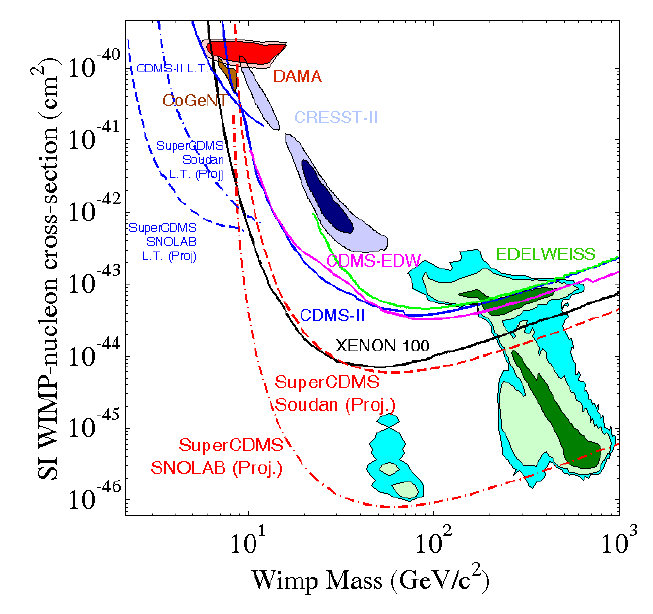
\includegraphics[width = .7\textwidth]{crosssection.png}
\caption{Upper limits on the spin-independent cross-section and WIMP mass parameter space as set by various dark matter experiments. The dash-dot line shows the projected upper limits for SuperCDMS SNOLAB due the the large detector payload (200kg) and increased detector. Figure from \cite{DOE}.}
\end{figure}

\chapter{SuperCDMS Soudan Tower}

This brief chapter discusses the design of the current tower in order to determine the design aspects we must consider in the SuperCDMS SNOLab tower. These include considerations for the charge and phonon read-out lines and the tower thermal stand-off tubes, which are being substantially re-designed for SuperCDMS SNOLab. A model of the current tower -- with the detector stack mounts -- is shown in Figure 2.1. This is the tower currently in use for the SuperCDMS Soudan experiment. The various components of the tower are described below, along with their design considerations.

\section{Tower Floor}
The bulk of the tower is made of OFHC (Oxygen-Free High Conductivity) Copper. This was chosen for its high thermal conductivity, dimensional stability, and high radio-purity. High thermal conductivity is required to ensure that the tower floors (and all devices heat sunk to them) are as close to the fridge stage temperatures as possible. Dimensional stability plays an important role during the cooldown of the experiment. If the tower's thermal contraction is too large, differential contraction can lead to either slack in the side-coaxes or stresses which can lead to thermal fatigue over multiple fridge run cycles. Lastly, a high radiopurity is required for all materials in the tower to minimize potential background in the experiment during operation.


\section{Heat Sinks to Dilution Fridge}

Excellent thermal links to each temperature stage of the fridge are necessary in order to maintain constant temperatures on the tower and enable effective heat dissipation. To achieve this, the current tower uses OFHC copper straps. These are composed of dozens of braided strands of well-annealed copper (RRR = 1200) which provide a large enough cross-section of copper to dissipate heat, but maintain flexibility, which prevents stresses from being created at the heat strap mount points \cite{Stockwell1996}.


\section{Tower Thermal Stand-offs}

The thermal stand-offs in the tower serve to thermally isolate each stage of the tower, while physically connecting the tower stages. The current experiment uses thin-walled graphite tubes between each stage, visible in Figure 2.1. These are nuclear-grade UF-4S graphite purchased from Mersen, milled to an OD of 1.99" with a 0.028" wall thickness. Apart from the wiring, these are the only structures which make inter-stage connections. The design of these is crucial, and comes from the intersection of numerous constraints: stiffness requirements, thermal loading limits, dimensional stability, radiopurity, and mechanical strength.

\begin{figure}[h]
\centering
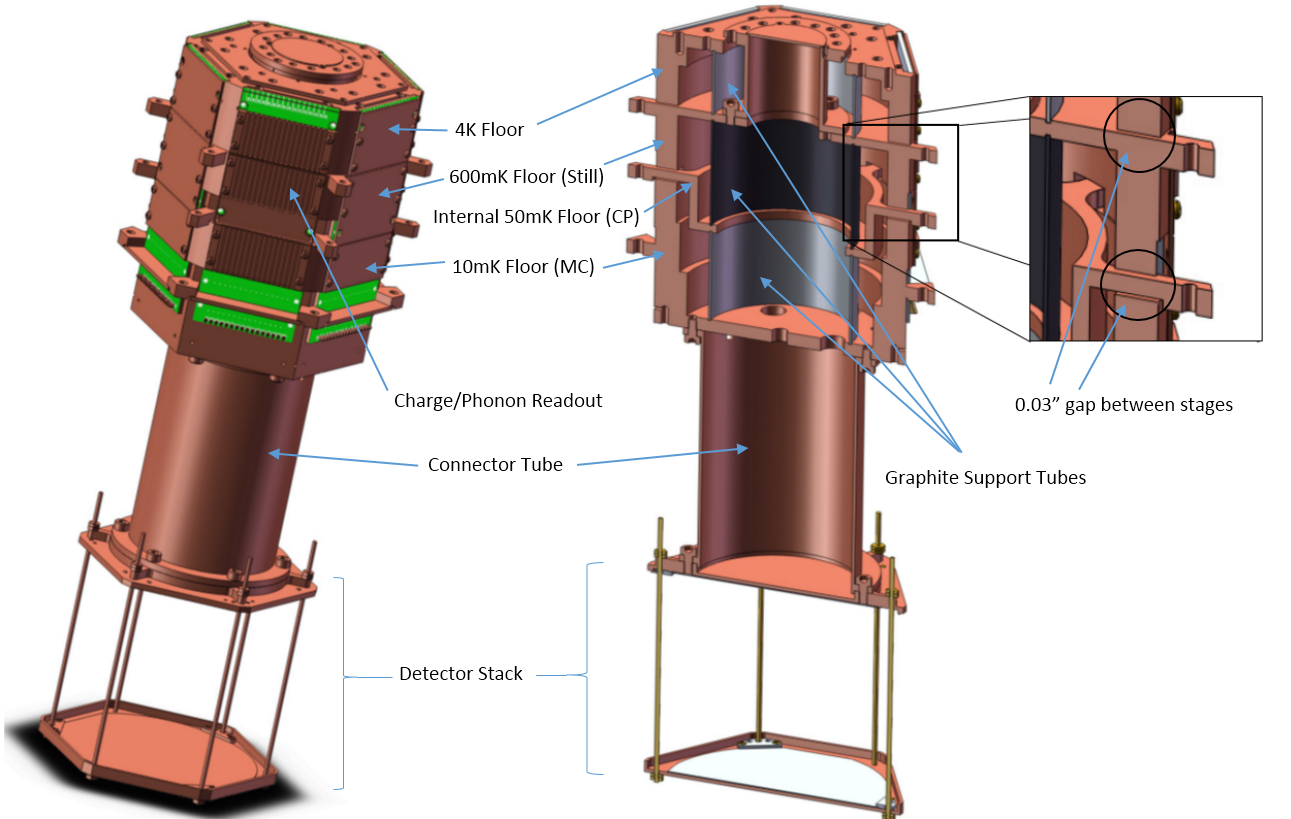
\includegraphics[width = .75\textwidth]{Labelled_tower.png}
\caption{Model of the SuperCDMS Soudan towers currently in use. The graphite support tubes and vacuum coax lines for charge/phonon readout are visible. The different thermal stages, which are thermally linked to the fridge, are visible in both models. These are 4K, 600mK (Still), 50mK (Cold Plate), 10mK (Mixing Chamber). Note that the 50mK stage is internal to the tower.}
\end{figure}

\subsection{Stiffness and Dimensional Stability}
The constraints on stiffness and dimensional stability stem from the requirement that the stage spacing doesn't change significantly during fridge operation. This is necessary for two reasons: First, it ensures correct operation and preservation of the vacuum coaxes. A tower which isn't sufficiently stiff can deform during handling, which could potentially damage the coaxes. A coefficient of thermal contraction which is too high can either create slack in the bare metal vacuum coax wires (shorting them to the tower) or cause stresses in the wires, which could plastically deform them \footnotemark. \footnotetext{see Appendix A for an investigation of stresses experienced by the NbTi vacuum coaxes which suggest large enough stresses to potentially result in plastic deformation.} Second, a low coefficient of thermal contraction for the stand-offs ensures that the different tower stages don't come into contact during cooling, which would create a thermal short between fridge stages\footnotemark. Graphite has very high dimensional stability, as well as a high enough modulus of elasticity to ensure a stable tower during cooldown and handling.

\footnotetext{This is not a concern for the new tower, which features a more open design and much larger stage separation.}

\subsection{Radiopurity}
The requirement for radiopurity in the thermal stand-offs come from the need to minimize background for our experiment. This is especially important for materials which are near the detectors, as there is little to no shielding to block radiation. The graphite in use is a nuclear grade graphite (very low impurity), which was shown to be very radioactively "clean" through a screening process (see section 4.3.2).

\subsection{Thermal Isolation}
One of the largest requirements of the thermal stand-offs is that they are very good insulators (low thermal conductivity) in order to ensure that heat flow between adjacent thermal stages of the tower is minimal. The UF-4S graphite used was shown to have very low thermal conductivity, so satisfied this requirement nicely.

\subsection{Mechanical Strength}
The tower supports were designed to be strong enough to withstand varied loads during handling and operation. This includes lifting/tilting the tower and supporting the detector stack in compression when mounted in the fridge. The symmetric tube shape of the supports ensures strength for many types of loads, and was proven to be very strong (it could support $\sim$145lbs when loaded in shear/bending!).


\section{Vacuum Coaxes}
Wiring must be routed down the side of the tower to the detector stack in order to control the detectors and read them out. The current design uses vacuum coaxes. These consist of .0012" diameter niobium-titanium (NbTi) wires suspended in rectangular grooves in the tower faces, which act as shielding. The grooves which encase each suspended wire are visible in the left image in Figure 2.1.

The vacuum coaxes were chosen for multiple reasons: First, they offer very low noise pick-up. This is critical when the signals being read-out from the detectors are so small. Second, they prevent any static charge build-up, which causes noise. Third, they minimize heat conduction between stages, because the bare NbTi wires are the only connection which is contiguous between all stages. This, in conjunction with the very low thermal conductivity of NbTi, provides very low heat conduction. Lastly, NbTi wires are superconducting below approximately 10K, which gives us zero resistance wiring to minimize signal loss before amplification and maintain a large phonon detection bandwidth.

\section{Connector Tube}
The tower connector tube is a cylindrical OFHC Copper tube which connects -- both physically and thermally -- the 10mK floor to the detectors. The purpose of this tube is two-fold: First, it roughly centers the detectors in the icebox of the fridge. This simplifies Monte Carlo simulations of detector performance. Second, it distances the radioactivity-sensitive detectors from the tower materials, which may be more radioactive than other materials in the experiment. Increasing the distance to the tower decreases the solid angle that the detectors subtend from the tower's position, which decreases the probability that an emitted radioactive particle will strike the detectors.

\section{Future Tower Considerations}
Though the design and technology used will change for the SNOLab tower, many of the considerations which went into designing the SuperCDMS Soudan tower will remain into the new design. As shown above, these considerations are numerous, and often competing (such as maximizing support strength while minimizing thermal conduction). Moving forward with the new tower design, these considerations should be kept in mind.



\chapter{Thermal Conductivity Tests}

Throughout the course of exploring and developing new options for tower designs, we conducted an immense literature search to determine the thermal conductivities of as many materials as possible to determine their suitability for use in the SuperCDMS SNOLab tower. There was often a problem with simply using the data in literature: measurements didn't cover the entire temperature range of interest, data presented was suspected to be inaccurate, preparation of the material measured wasn't the same as our own (e.g. various heat treatments). Often, due to our desire to use new or little-known materials, there was no thermal conductivity data in the literature at all. This required us to design and carry out a series of thermal conductivity tests. This chapter presents the thermal conductivity tests which were carried out in our lab in our 75$\mu$W helium dilution refrigerator.

\section{Motivation to Conduct Tests}
The next generation of the CDMS Experiment -- SNOLab -- will require a significant improvement in cold hardware thermal performance to fall within the cooling power of the dilution fridge which will be used. We are at the edge of this threshold now with our current designs, and are therefore very sensitive to the thermal properties of our candidate materials. It is for this reason that we wish to characterize precisely the thermal conductivity of all our candidate materials for the entire temperature range in which we are considering using them. Below, I describe the tests which have been conducted, the tests which will be conducted, and the reason for our interest in the materials.

\subsection{Vespel SCP-5000 and SCP-5050}
The DuPont Vespel SCP series materials can be seen as the "updated" SP series from the same manufacturer. SCP-5000 and SCP-5050 are similar to SP-1 and SP-22, respectively, except with higher strength and thermal stability (i.e. lower coefficient of thermal expansion). Given the popularity of Vespel SP products in cryogenic support systems, this naturally makes the SCP series very attractive as tower stand-off materials.

\subsection{Graphlite Carbon Fiber}
Graphlite is a trade name for carbon fiber reinforced plastic (CFRP) -- which is well known for its strength. This material has shown to have an impressively high compressive/tensile strength which would be exploited in a truss structure. A very similar material has been characterized by Marc Runyan at larger diameters and higher temperatures \cite{run}.

\subsection{Ti 15-3-3-3}
Ti 15-3-3-3 is an alloy of titanium originally developed by TIMETAL with composition 15V-3Sn-3Al-3Cr and Ti as a balance. This material has been measured previously in plate form and has shown to have very interesting (and very low) thermal conductivity at low temperatures. In addition, it is a very strong alloy with a low thermal expansion coefficient and superconducting properties. We have interest in Ti 15-3-3-3 in plate, tube, and foil form. We have looked into multiple sources for these forms, each of which must be characterized, due to the different manufacturing processes present in the production of each.

\subsection{Mersen Graphite Grade 2020}
Mersen's grade 2020 graphite is interesting to us for multiple reasons. First, Mersen manufacturers the graphite we currently use, grade UF-4S, which has low thermal conductivity and high purity. Second, it is a nuclear grade graphite, so should have very low radioactivity -- a necessity in our experiment. Third, this grade was specifically recommended to us, by the R\&D and Technical Manager at Mersen as well as their resident graphite expert, to satisfy low radioactivity and low thermal conductivity requirements.

\subsection{POCO Graphites}
POCO manufactures many grades of graphites. One of their industrial grades, AXM-5Q has demonstrated very low thermal conductivity. We wish to characterize some of their other industrial grades, ACF-10Q and ZXF-5Q, which may offer similar thermal qualities. Though these graphites are industrial grade, we have demonstrated that they may be purified to acceptable levels of radioactivity (see section 4.3.2).

\begin{figure}[h]
\centering
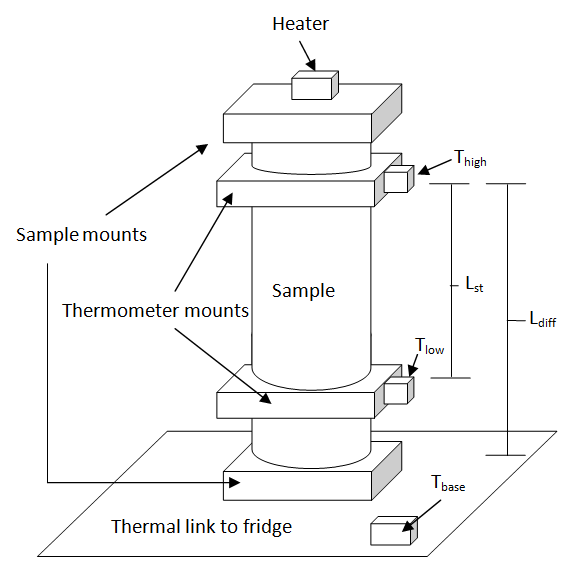
\includegraphics[width = .5\textwidth]{C:/Users/Niko/Documents/LaTex/Nick_K_Thesis/CH5_figs/Rep_test_setup.png}
\caption{Representative test set-up for thermal conductivity tests performed in the 75$\mu$W dilution fridge. The sample mounts were gold-plated copper for all samples except the Ti 15-3-3-3, which was unplated copper. All thermometer mounts were copper. Primarily two thermometers ($T_{high}$ and $T_{low}$) were used for measurements, but a third ($T_{base}$) was mounted on the thermometry package attached to the tower to verify fridge base temperatures throughout some measurements. }
\end{figure}
\section{Experimental Test Set-up}
The thermal conductivity tests were conducted in a 75-$\mu$W 3He-4He dilution refrigerator. A representative experimental set-up is shown in Figure 3.1. The samples were connected on one end (through multiple copper-copper interfaces) to the mixing chamber of the fridge, while the other end was thermally isolated.

\subsection{Heater}
The heater was a metal film resistor, which offers high stability over large temperature ranges. Power was applied to the heater through a Keithley 213 Quad Voltage Source. The resistance was initially 2$k\Omega$, but was later switched to 20$k\Omega$ to allow greater resolution in the voltage applied to the heater, due to the internal 0.25mV minimum step size from the Keithley. The first Graphlite measurement, Vespel SCP-5050, and Vespel SP-22 used the 2$k\Omega$ heater.

\subsection{Thermometry}
Temperature was read out by either two or three thermistors, depending on the test. $T_{high}$ and $T_{low}$ were used in every test; $T_{high}$ and $T_{low}$ were Germanium thermistors. $T_{base}$ was used in some tests to verify the base temperature of the fridge and was a RuO$_{2}$ thermistor. Voltage bias to the thermometers was provided through the Keithley 213 Quad Voltage Source. $T_{high}$ and $T_{low}$ were both four-wire connections for accurate resistance readout.

\subsection{Wiring}
All electrical connections were initially .003" diameter manganin wires, $\approx$ 8 inches long. The initial Graphlite measurement, as well as the Vespel SCP-5050 and SP-22 measurements were preformed with this wiring. Subsequent tests switched to .0012" manganin wires with a Formvar coating for the heater and $T_{high}$ connections in order to minimize parasitic heat loads. For the samples tested to date, the parasitic heat load from wiring is estimated to be no more than 14\% (for the lowest temperature data points for Vespel SCP-5050). It was usually less than $\sim$3\% for the experiments.

\subsection{Mounting}
The samples were epoxy-ed with Stycast-1266 into gold-plated-copper mounts for improved heat transfer from the heater, through the sample, to the fridge.

Separate thermometer mounts were fabricated and placed along the sample to avoid any Kapitza resistance effects caused by placing thermometers on the same block as the heater. The thermometer mounts were placed far enough along the sample to be confident that planar heat flow had been established by the time temperature was read out.

\section{Methods for Measuring Thermal Conductivity}
The thermal conductivity of our samples was measured using three methods which I have termed the "differential" method, the "standard" method, and the "parameter-fit" method. The standard method and the parameter-fit method utilize the same measurements, but different analysis methods, while the differential method is different altogether. All three are outlined below.

\subsection{Differential Method}
This method for measuring thermal conductivity involves two successive measurements to provide one thermal conductivity data point. First, power $P_1$ is applied to the sample to establish a gradient, with the "hot" thermometer at some $T_{high_1}$. Then, more power, $P_2$, is applied to the sample which raises the "hot" thermometer to $T_{high_2}$. Throughout these two measurements, we assume a good enough thermal link to the fridge such that the base of the sample remains roughly constant (whether or not it is at $T_{base}$). The gradient of interest in both cases is $T_{high}$ to whatever temperature the base of the sample is at (for simplicity we will call it $T_{base}$). Then in steady state, the power through the sample is,
\begin{eqnarray}
P = \int_{T_{base}}^{T_{high}} \frac{A}{L_{diff}}K(T)dT
\end{eqnarray}
where $T_{base}$ is the temperature of the cold end of the sample, $T_{high}$ is the temperature of the top thermometer, A is the cross-section of the sample, $L_{diff}$ is the length from the hot thermometer to the base of the sample as shown in Figure 3.1, and K(T) is the thermal conductivity of the sample. From here, we subtract $P_1$ from $P_2$ to obtain an effective integral,
\begin{equation}
    \begin{aligned}
P_2 - P_1 & = \left(\int_{T_{base}}^{T_{high_2}} \frac{A}{L_{diff}} K(T)dT - P_{parasitic}\right) \ - \ \left(\int_{T_{base}}^{T_{high_1}} \frac{A}{L_{diff}} K(T)dT - P_{parasitic}\right) \\
& = \int_{T_{high_1}}^{T_{high_2}} \frac{A}{L_{diff}} K(T)dT \ .
    \end{aligned}
\end{equation}
Here we assume that the thermal conductivity is some integrable function with the same form in both integrals, and $P_{parasitic}$ is some constant parasitic contribution to the heat load (from noise, etc.). Then, upon integration, the value of the integral at the lower limit, $T_{base}$, cancels out in both integrals, leaving the effective integral at the right of the last equal sign. So, given $P_2 - P_1 = \Delta P$, the differential power, we calculate the thermal conductivity at,
\begin{eqnarray}
T_{avg} = \frac{T_{high_1} + T_{high_2}}{2}
\end{eqnarray}
by assuming K(T) is nearly constant over the range $T_{high_1} \rightarrow T_{high_2}$ so that it can be brought outside of the integral,
\begin{eqnarray}
\Delta P = K_{T_{avg}}\frac{A}{L_{diff}}\int_{T_{high_1}}^{T_{high_2}}dT \ .
\end{eqnarray}
Integrating and rearranging, we have,
\begin{eqnarray}
K_{T_{avg}} = \Delta P\frac{L_{diff}}{A(T_{high_2}-T_{high_1})} \ .
\end{eqnarray}
This method has several advantages and disadvantages:
\bigskip

\textbf{Advantages}
\begin{itemize}
\item As can be seen from eqn 3.2, any constant parasitic heat load can be neglected with this method, making low temperature measurements (with low applied powers) much easier.
\item Since this method only uses one thermometer to do temperature measurements ($T_{high}$), it eliminates any relative calibration error between thermometers, such as may be present between $T_{high}$ and $T_{low}$.
\item It allows the measurement to be conducted over very small effective gradients ($T_{high_1} \rightarrow T_{high_2}$) so the constant thermal conductivity approximation used in eqn 3.4 is more accurate, even for strongly temperature-dependent thermal conductivities.
\end{itemize}

\bigskip

\textbf{Disadvantages}
\begin{itemize}
\item The differential method requires a very good thermal link to the cooling bath/a fridge with a high cooling power. This is to ensure that $T_{base}$ is roughly constant between two consecutive measurements. The error from a varying $T_{base}$ is amplified in shorter samples.
\end{itemize}

We found the differential method to disagree with the following two methods in many instances. We believe that this was due to poor thermal links to the fridge with these samples, caused by inadequate gluing.

\subsection{Standard Method}
Though there is obviously no "standard" method for measuring thermal conductivity, I refer to this as the standard method as it is the most straight-forward of the steady heat-flow measurement methods. This involves applying a power, $P_{heater}$, to the top of the sample and letting the sample reach equilibrium (which took anywhere from 30 minutes at higher temperatures to 90 minutes at the lowest temperatures) according to the steady-state heat flow equation,

\begin{equation}
    \begin{aligned}
P & = P_{heater} + P_{parasitic}\\
  & = \int \frac{A}{L_{st}} K(T)dT\\
    \end{aligned}
\end{equation}
where A is the cross-section of the sample, $L_{st}$ is the length between the two thermometers, given in Figure 3.1, K(T) is the temperature-dependent thermal conductivity of the sample, and $P_{parasitic}$ is any other parasitic heat load through the sample. Reading out the temperatures $T_{high}$ and $T_{low}$, and assuming that K(T) is nearly constant over this temperature range, we bring K(T) out of the integral as in eqn 3.4 and integrate. After rearranging we have,
\begin{eqnarray}
K_{T_{avg}} = P\frac{L_{st}}{A(T_{high} - T_{low})} \ ,
\end{eqnarray}
where $K_{T_{avg}}$ is assumed to be the thermal conductivity at some $T_{avg}$ (defined in eqn 3.3).

The standard method has its own set of advantages and disadvantages, which are outlined below.

\bigskip

\textbf{Advantages}
\begin{itemize}
\item This method is simple, with no assumptions about good thermal links to cooling baths, etc.
\end{itemize}

\textbf{Disadvantages}
\begin{itemize}
\item There is a high sensitivity to relative calibration errors between $T_{high}$ and $T_{low}$ for small temperature gradients, which makes measurements at lower temperatures difficult.
\item Constant parasitic heat loads -- if not adjusted for in calculations -- can be larger than applied heat loads for low temperature ranges, giving hugely inaccurate results for K. The effects of these heat loads can be minimized by either increasing the geometric factor A/L to increase applied heat loads through the sample (decreasing the percentage of power coming from parasitic sources), or by measuring and accounting for $P_{parasitic}$ in calculations.
\item Errors from the constant thermal conductivity approximation can grow quickly at large gradients, especially for strongly temperature-dependent thermal conductivities. However, for most thermal conductivities, gradients of over 100\% of $T_{high}$ can be used with minimal errors\footnotemark.
\end{itemize}

\footnotetext{See \cite{Hust1982} for a discussion of these errors.}

\subsection{Parameter-fit Method}
The parameter-fit method is similar to the standard method in that a power is applied to that sample, and $T_{high}$ and $T_{low}$ are read out once equilibrium is reached. We start
 from eqn 3.6, but instead of assuming a constant K, we assume some integrable form for K(T) -- often a power law of the form $A \cdot T^B$ at sub-kelvin temperatures. We can then vary a set of parameters (e.g. A and B in the power law form) to find those which minimize the quantity,
\begin{eqnarray}
\Delta = \sum_{i = 1}^{n} \left[\frac{P_{total_i} - P_{expected_i}}{P_{total_i}}\right]^2
\end{eqnarray}
for $n$ measurements. $P_{total_i} = P_{heater_i} + P_{parasitic_i}$ is a combination of the power applied to the heater and any parasitic heat loads, and $P_{expected_i}$ is given by,
\begin{eqnarray}
P_{expected_i} = \int_{T_{low_i}}^{T_{high_i}} \frac{A}{L_{st}}K(T)dT
\end{eqnarray}
with $T_{high_i}$ and $T_{low_i}$ being the high and low thermometer temperatures for a given measurement and K(T) is the assumed form for thermal conductivity with certain parameter values. $\Delta$ will vary as you vary parameter value combinations. Whichever values minimize this quantity are the best fit to the data.

The standard method approaches the parameter-fit method in the limit of very small gradients, therefore they share similar advantages and disadvantages.

\bigskip

\textbf{Advantages}
\begin{itemize}
\item Since this method makes no assumptions about a constant thermal conductivity (unlike the standard method), it isn't susceptible to error for large gradients.
\item It makes no assumptions about a perfect thermal link to a reservoir.
\end{itemize}

\textbf{Disadvantages}
\begin{itemize}
\item Since both the high and low thermometers are used, low gradient measurements are sensitive to relative calibration errors between thermometers.
\item The data is sensitive to constant parasitic heat loads which can introduce large errors when $P_{parasitic}$ is comparable to $P_{heater}$.
\item This method forces the data to be fit to an assumed form, so the data is inherently more "processed" by the time it is viewed. This could gloss over any anomalous behavior in the material's conductivity curve. Most materials' thermal conductivity, however, can be fit to a power law at low temperatures, so this isn't always a problem.
\end{itemize}

\section{Measured Thermal Conductivities}
The thermal conductivities of five samples has been measured as of \today. These are: Graphlite carbon fiber, Vespel SCP-5050 \& SCP-5000, Vespel SP-22, and Ti 15-3-3-3. The results of each measurement are presented below with a brief discussion following. Note that error bars on the plots have only been included for the standard method.

\subsection{Graphlite}

The thermal conductivity of a 0.156" diameter Graphlite rod was measured from 0.05K to 0.5K using the three methods described above. The plot is shown in Figure 3.2. The agreement between all three methods is very good for the case of the Graphlite, as the thermal contact between the fridge and the sample was very good. The parameter-fit method in this case was fit to an altered power law of the form,
\begin{eqnarray}
K(T) = A \cdot T^{(B - C \cdot T^{D})}
\end{eqnarray}
which is the same form fitted to in a previous measurement by M. Runyan in \cite{run}. The parameter-fit method, shown in Figure 3.2, gave a thermal conductivity of,
\begin{eqnarray}
K(T) = 101.2 \cdot T^{(1.93 - 1.15 \cdot T^{0.28})} \ \frac{\mu W}{cm-K}
\end{eqnarray}
for the data range. This is noticeably higher than was measured in \cite{run}. This could be due to the fact that the larger diameter sample measured by M. Runyan was not the "official" Graphlite, as Graphlite is only manufactured up to 0.156" diameter.

\subsection{Vespel SCP-5050}

The thermal conductivity of Vespel SCP-5050 was measured from 0.09K to 0.5K. The results are shown in Figure 3.3 below. Once again, all three methods are in very good agreement, with the parameter-fit method giving a power law fit of
\begin{eqnarray}
K(T) = 10.78 \cdot T^{1.90} \frac{\mu W}{cm-K} \ .
\end{eqnarray}

\subsection{Vespel SP-22}
The thermal conductivity of Vespel SP-22 was measured from 0.1 to 0.3K. The results are plotted and compared to previous measurements of this material in Figure 3.4. With this sample we can clearly see that the differential measurement is not in agreement with the other two methods. We hypothesize that this was due to a poor thermal link to the fridge caused by improper gluing. We discovered this as the sample broke free of its base mount on the fridge connection side during disassembly with almost no applied force. The break is shown in Figure 3.5.

The parameter-fit method used a power law fit and gave a thermal conductivity of,
\begin{eqnarray}
K(T) = 13.3 \cdot T^{1.73} \frac{\mu W}{cm-K}
\end{eqnarray}
which is shown to be in very good agreement with previous measurements of SP-22.

This test was primarily a confirmation of our Vespel SCP-5050 results as it confirmed the accuracy of our test set-up. The equipment used in both tests was identical (same heater, wiring, sample dimensions, etc.) so is a strong confirmation of the SCP-5050 results.

\begin{SCfigure}
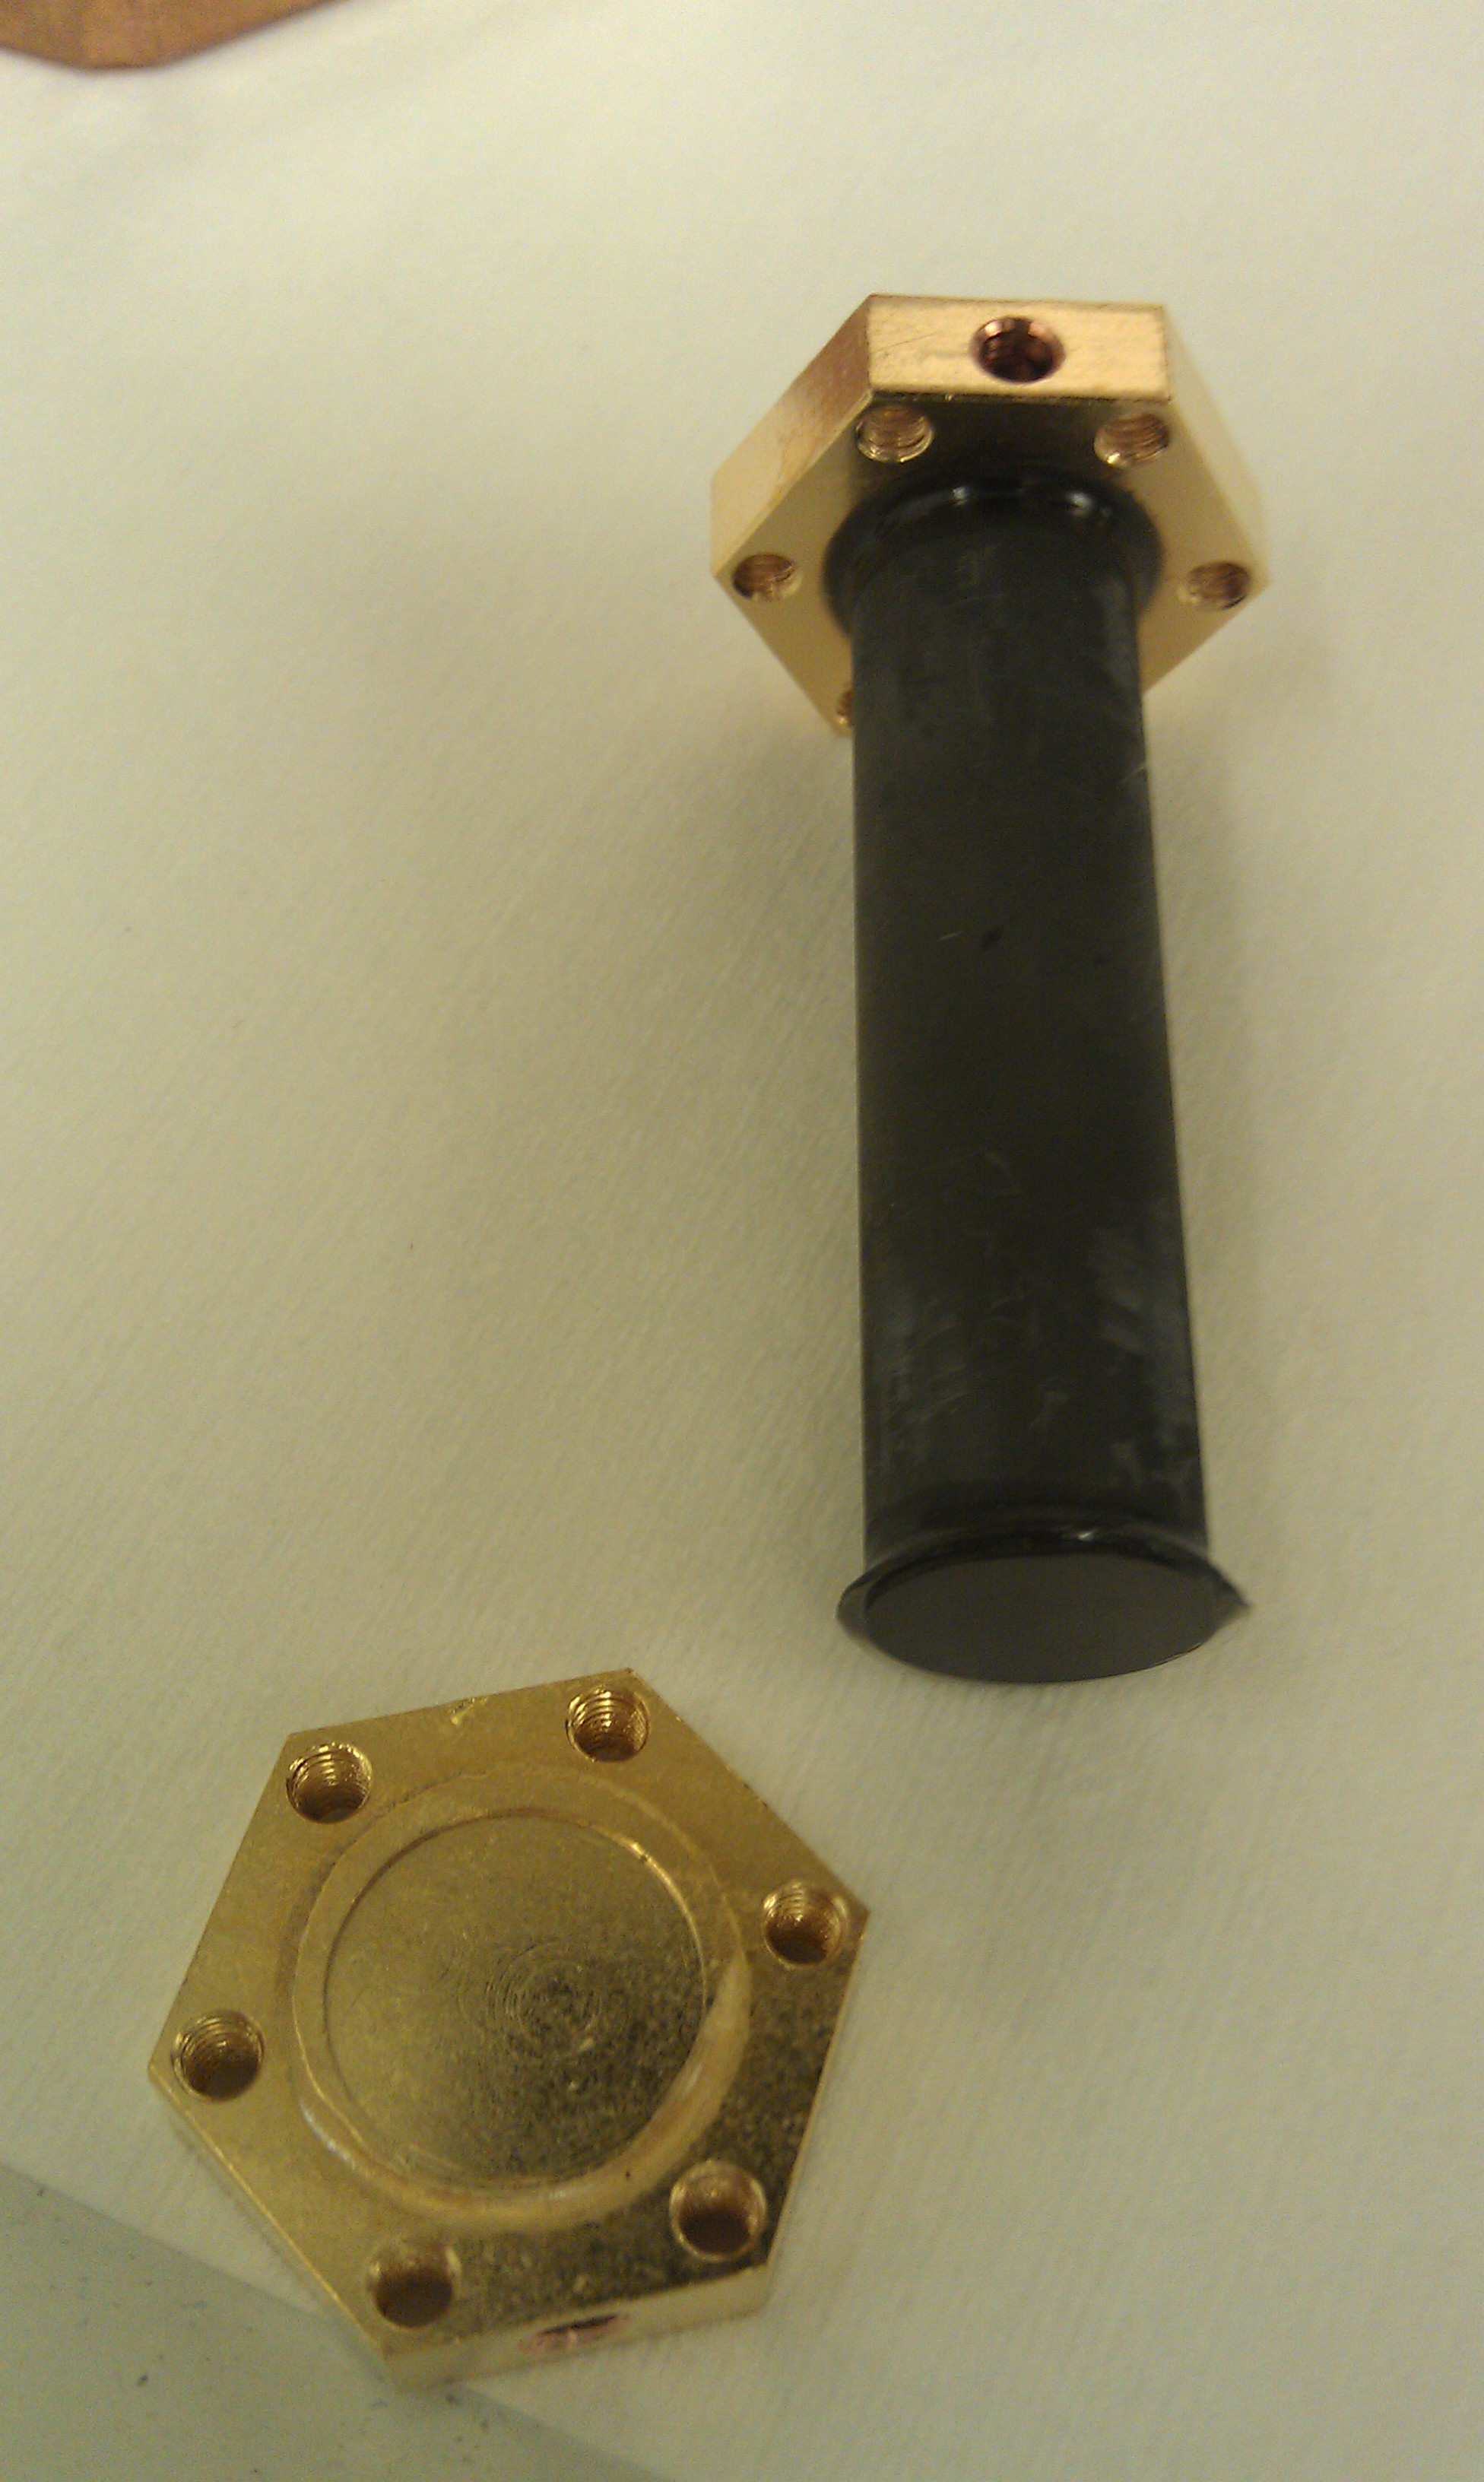
\includegraphics[width = .2\textwidth]{C:/Users/Niko/Documents/LaTex/Nick_K_Thesis/CH5_figs/broken_sp22.jpg}
\caption{The SP-22 sample-mount interface broke during removal from the fridge. This occurred with hardly any applied force on the sample. This was the interface which defined the thermal link to the fridge and was likely the cause of the discrepancy between the differential method and other methods shown in Figure 3.4.}
\end{SCfigure}

\subsection{Vespel SCP-5000}
The thermal conductivity of Vespel SCP-5000 was measured from 0.09K to 0.55K using the three methods described in the previous section. Here, the tests were conducted slightly differently, with two differential measurements being performed instead of one. This involved the differential measurement using the $T_{high}$ thermometer only, but also a separate measurement which utilized the $T_{low}$ thermometer only. This resulted in two differential measurements on different effective sample lengths (one from $T_{high}$ to base and one from $T_{low}$ to base). The results are shown in Figure 3.6.

In the figure, we see a huge discrepancy between the two differential measurements, as well as between the differential measurements and the other methods. This was likely due to very poor thermal contact with the fridge (possibly caused by untightened mounting screws, or poor gluing). This is evidenced by the fact that the short- sample differential method (using $T_{low}$ suffered a greater error than the long-sample measurement. This test will be re-run at a later date to attempt to rectify this discrepancy.

The parameter-fit method and standard method are once again in good agreement, with the parameter-fit giving a thermal conductivity of,
\begin{eqnarray}
K(T) = 15.2 \cdot T^{1.12} \frac{\mu W}{cm-K} \ .
\end{eqnarray}

\subsection{Ti 15-3-3-3}
The thermal conductivity of Ti 15-3-3-3 is of interest for reasons described in section 1. Since billets of Ti 15-3-3-3 are not available in the United States, we purchased a round billet of Ti 15-3-3-3 from ReTi in China. It the the thermal conductivity of this material which is presented here from 0.07K to 0.3K.

The results of this measurement are shown in Figure 3.7, alongside measurements of similar samples. We see from the figure that the agreement between the three methods is fair in this case, but there is still a visible discrepancy between the differential method and the other two methods. The reasons for this discrepancy are unknown, but are likely due to a less-than-ideal thermal link to the fridge.

The parameter-fit method gave a thermal conductivity of,
\begin{eqnarray}
K(T) = 187.4 \cdot T^{1.82} \frac{\mu W}{cm-K}
\end{eqnarray}
which is in good agreement with the measurements performed by M. Runyan on a similar bulk sample of Chinese-sourced Ti 15-3-3-3. The interesting thermal behavior exhibited by TIMET's Ti 15-3-3-3 is not present in this sample, making it much less desirable as a stand-off material.\footnotemark

\footnotetext{We believe that the thermal conductivity of TiMetal Ti 15-3-3-3 exhibits a lower thermal conductivity than the ReTi Ti 15-3-3-3 at low temperatures; we are not as confident that the thermal conductivity drop is as extreme as it appears in the plot. To get this curve, the authors of \cite{wik} used a parameter-fit method was employed. The last data point, however, was with a gradient from $\sim$ 650mK to 230mK. Fitting such a large area with one measurement could lead to large errors depending on the fit used or if there were unknown parasitics.}


\subsection{Thermal Conductivities of All Materials}
The parameter-fit thermal conductivities of all tested materials are presented in Figure 3.8. We see a large span for the thermal conductivities of the materials tested. We plan to test more samples in the near future to further characterize the various materials we plan to use, or may decide to use, for the SNOLab tower development.

\begin{figure}[h]
\centering
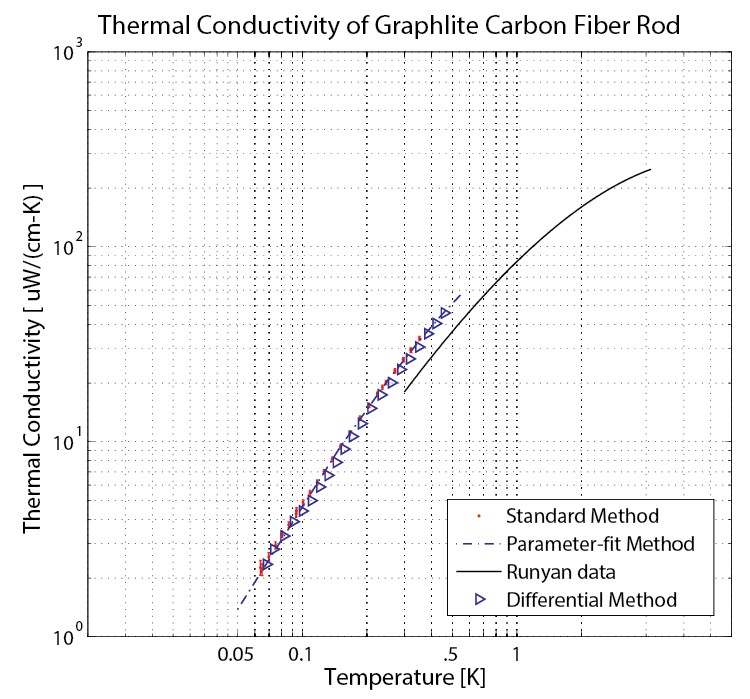
\includegraphics[width = .8\textwidth]{C:/Users/Niko/Documents/LaTex/Nick_K_Thesis/CH5_figs/Graphlite.png}
\caption{Thermal conductivity of Graphlite from 0.05K to .5K as measured at UC Berkeley. The results are show reasonable agreement with a previous measurement of Graphlite by M. Runyan, plotted as the solid (\textbf{--}) black line \cite{run}. The disagreement could be due to the fact that the sample measured by M. Runyan was not "official" Graphlite, though it was provided by the same company.}
\end{figure}

\begin{figure}[h]
\centering
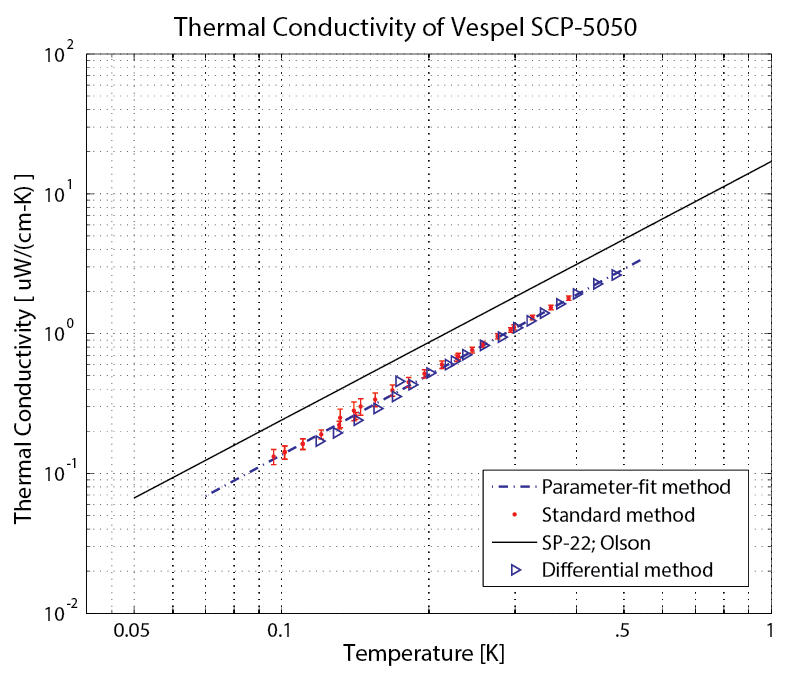
\includegraphics[width = .8\textwidth]{C:/Users/Niko/Documents/LaTex/Nick_K_Thesis/CH5_figs/SCP5050.png}
\caption{Thermal conductivity of Vespel SCP-5050 as measured from 0.09K to 0.5K. This data is compared to previous measurements of Vespel SP-22 (a very similar material, which we hope SCP-5050 can improve upon) by J.R. Olson \cite{ols}. SCP-5050 is noticeably lower ($\sim$ 30\%) in thermal conductivity.}
\end{figure}

\begin{figure}[h]
\centering
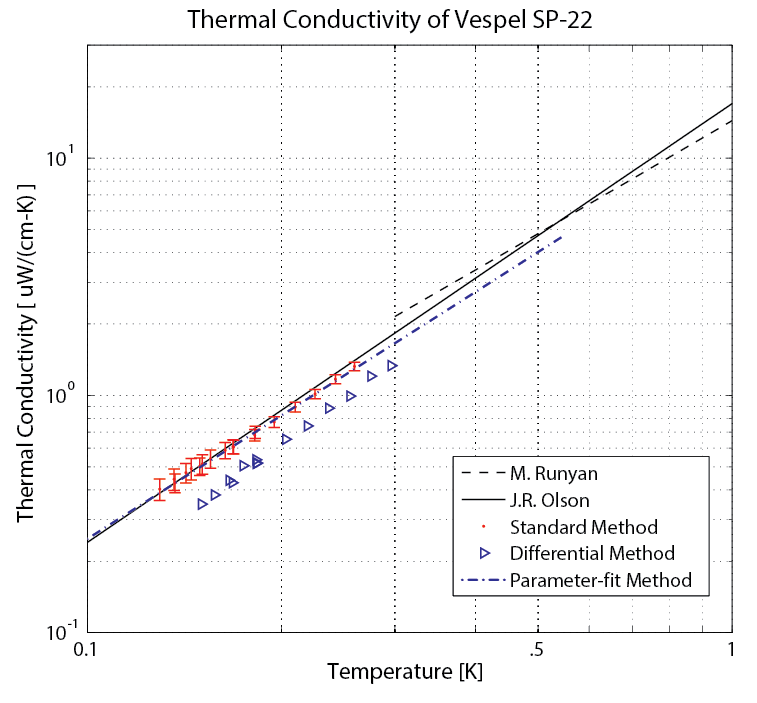
\includegraphics[width = .8\textwidth]{C:/Users/Niko/Documents/LaTex/Nick_K_Thesis/CH5_figs/SP22.png}
\caption{Thermal conductivity measurements of Vespel SP-22 as compared to previous measurements by J.R. Olson \cite{ols} and M. Runyan \cite{run}. Our data agree with these previous results very well. The uncertainty presented for the standard method are very conservative, and are likely lower. }
\end{figure}

\begin{figure}[h]
\centering
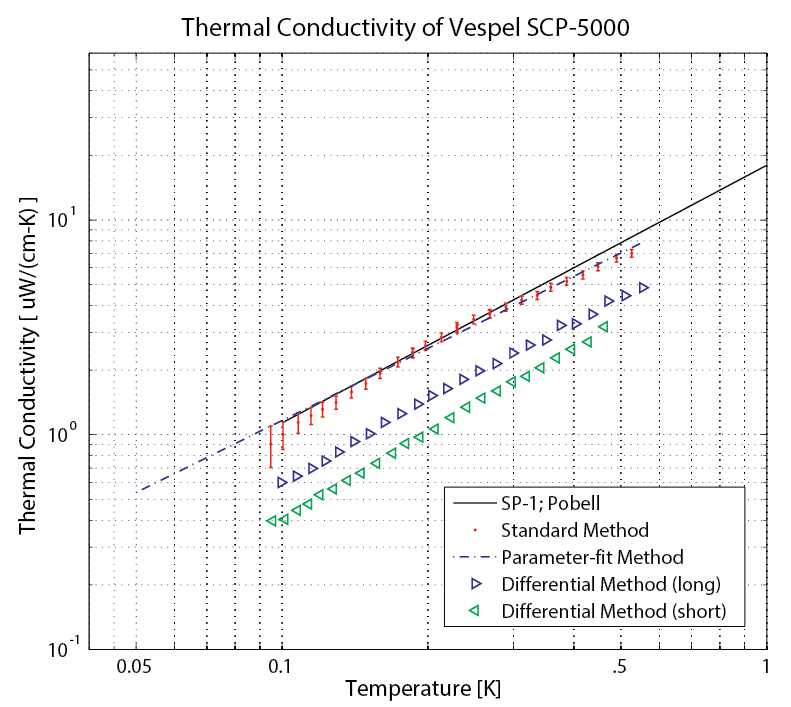
\includegraphics[width = .8\textwidth]{C:/Users/Niko/Documents/LaTex/Nick_K_Thesis/CH5_figs/SCP5000.png}
\caption{Thermal conductivity of Vespel SCP-5000 from 0.09K to 0.55K. This is compared to measurements of Vespel SP-1 taken from Pobell \cite{pob}. The agreement is very good. The differential measurements in this test were not in good agreement. This may have been due to a large contact resistance or simply poor thermal contact between the fridge and the sample; this would cause the assumption of constant base temperature between measurements to not hold true.}
\end{figure}

\begin{figure}[h]
\centering
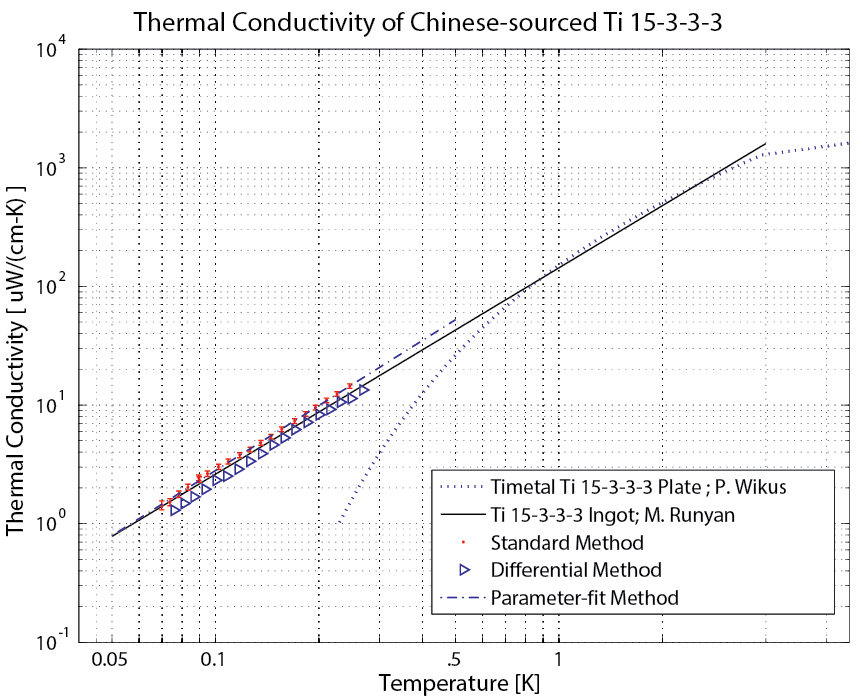
\includegraphics[width = .8\textwidth]{C:/Users/Niko/Documents/LaTex/Nick_K_Thesis/CH5_figs/Ti15333.png}
\caption{Thermal conductivity of ReTi Ti 15-3-3-3 from 0.07K to 0.3K. There is a slight discrepancy between the differential method and the parameter-fit/standard methods. The agreement with the Chinese-sourced Ti 15-3-3-3 sample measured by M. Runyan is good. The interesting thermal conductivity behavior exhibited by TIMETAL's Ti 15-3-3-3 plate measured by Wikus in \cite{wik} is not present in this sample.}
\end{figure}

\begin{figure}[h]
\centering
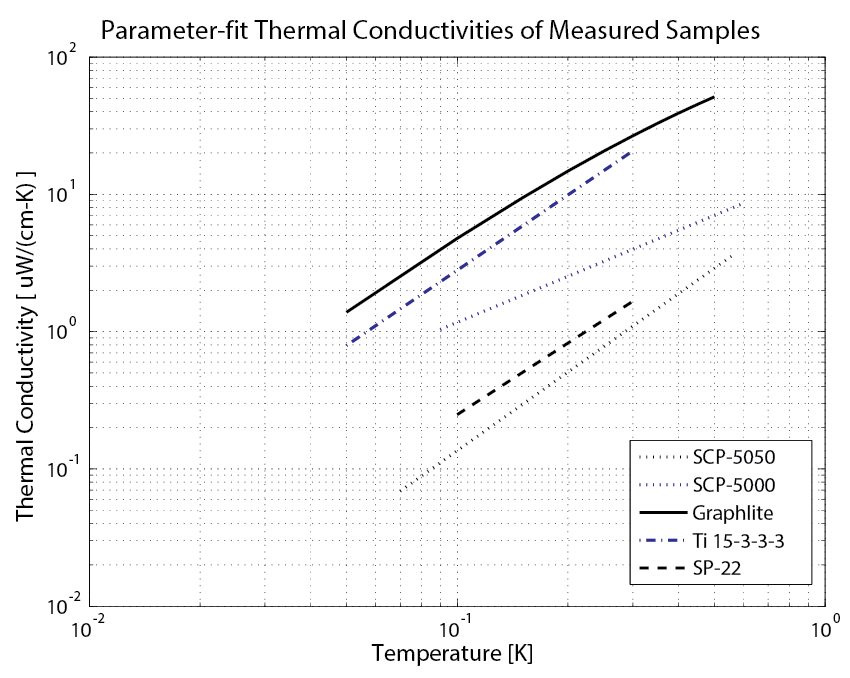
\includegraphics[width = .9\textwidth]{C:/Users/Niko/Documents/LaTex/Nick_K_Thesis/CH5_figs/all.png}
\caption{Compiled thermal conductivities of all measured materials. The plots given are the parameter-fit lines for each sample tested.}
\end{figure}

\subsection{Three methods for measuring thermal conductivity}

Through these tests, we have seen that all three methods for calculating thermal conductivity can provide accurate data; each has its own set of advantages and disadvantages which it confers. The differential measurement isn't susceptible to constant parasitic heat loads (often the dominating source of noise for measurements at the lower limits) and requires only one thermometer; however, it requires a very good thermal link to a cooling reservoir to be valid. The standard method is a reliable method which produces good results even for large gradients across the sample, and isn't as dependent on thermal links to the cooling reservoir as the differential method, but makes it more difficult to account for parasitic heat loads. It also won't won't at large gradients for highly temperature-dependent thermal conductivities. The parameter-fit method offers many of the advantages and disadvantages of the standard method, but allows very large gradients to be used, as it doesn't assume a constant thermal conductivity along the length of the sample. It does, however, require one to assume an equation for for the thermal conductivity, so can introduce a data bias.

Overall, if one can assure a strong thermal link to a cooling reservoir (which can be verified through a second thermometer on the cold end of the sample), we would recommend the differential method of measurement for samples, due to its immunity to many parasitics. Ideally, however, multiple methods would be used in a given test to cross-check data.

\chapter{Tower Thermal Stand-off Design}

As stated in the previous chapter, the thermal stand-offs for our detector tower are designed primarily to support the detector stack and electronic connections, while thermally isolating the various 4He-3He dilution fridge temperature stages -- apart from wiring, these stand-offs are the only inter-stage connections on the tower. However, any tower support structure must address numerous concerns in its design; These concerns are: thermal conductivity, radiopurity, thermo-mechanical properties such as strength, elastic moduli, and expansion coefficients, and -- for the design of the structure itself -- the ability to withstand various loads and shocks without failure. In this chapter, I explore various stand-off candidates which offer significant improvements over our current UF-4S graphite tubes based on their merits of thermal conductivity, radiopurity, and their thermo-mechanical properties. From here, I consider two design possibilities for the stand-off geometry: thin-walled cylindrical shells and hexapods. An analytical model for the thin-walled shells -- or "tubes" -- is developed in an effort to further improve fridge performance by optimizing tube dimensions to minimize heat load while maximizing strength. We find that new designs for SuperCDMS SNOLAB may be able to reduce interstage heat loads from the thermal stand-offs by nearly a factor of twenty.

\section{Candidate Materials}
The numerous parameters which our thermal stand-off materials must satisfy gives us a list of equally numerous candidate materials, each of which is known -- or believed -- to satisfy at least some of the requirements (that they satisfy other requirements is proven in the following sections). This section identifies the various candidates and describes their merits as stand-off materials.

\subsection{DuPont Vespel}
Vespel is a polyimide-based material produced by DuPont which is widely used in both high-temperature, and cryogenic applications. The polyimide is a condensation type produced from pyromellitic dianhydride (PMDA) and 4,4' diamino diphenyl ether (ODA)\footnotemark. We are considering four compounds of Vespel for this experiment: SP-1,SP-22,SCP-5000, and SCP-5050. The SP-series compounds are estimated to have a crystallinity of between 25 and 50\%.

\footnotetext{Information from DuPont literature: Vespel S line Design Handbook}

Vespel SP-1 is the unfilled polyimide resin. This compound has low thermal conductivity, is high strength, and has demonstrated low levels of radioactivity. SP-1 has a low dimensional stability, however, with a high coefficient of thermal expansion (CTE) an low elastic moduli.

Vespel SP-22 is the base polyimide, SP-1, filled with 40\% graphite by weight. This material is even lower thermal conductivity than SP-1, making it an ideal candidate. In addition it offers higher dimensional stability than SP-1, with a lower CTE and higher moduli of elasticity. Unfortunately, it demonstrates a high level of radioactivity which probably originates from the graphite used.

Vespel SCP-5000 is an unfilled polyimide resin very similar to SP-1, however it has been engineered to have higher strength and improved dimensional stability. This includes a lower CTE and significantly higher elastic moduli. At the same time, we have shown that SCP-5000 has a thermal conductivity as low as SP-1.

Vespel SCP-5050 is analogous to SP-22 in that its composition is base resin (SCP-5000) filled with 40\% graphite by weight. It is not as strong as SCP-5050, but offers the highest dimensional stability of the Vespel compounds being considered; its CTE is designed to be similar to steel. In addition, it demonstrates a lower radioactivity and lower thermal conductivity than SP-22.

All the Vespel compounds are being considered as isostatically formed parts, rather than direct formed, because this ensures isotropic structure and properties. Direct formed parts are created with a process similar to powder metallurgy, which leaves them with anisotropies. This has consequences for the material properties, such as a tensile strength and elongation which are lower in the direction parallel to the moulding force.

\subsection{Graphite}

Our current thermal stand-off material, grade UF-4S from Mersen, is graphite for many reasons. Graphite is known to have a very low thermal conductivity, and high dimensional stability. Its radioactivity can be minimized by purchasing nuclear grades, or by purification processes such as the one described in section 3.3.2 which reduce radioactive contaminants to very low levels.

The first graphite candidate is Grade 2020 from Mersen. This material was recommended to us by the R\&D manager at Mersen for low thermal conductivity and high strength/purity. It is a nuclear grade graphite which can be further purified, and demonstrates reasonable radioactivity levels. It has a high dimensional stability, and is stronger than UF-4S graphite.
The next graphite grade being considered is AXM-5Q\footnotemark, an industrial grade graphite produced by POCO. This material exhibits even lower thermal conductivity than UF-4S graphite (section 3.2) and higher strength. Off the shelf, this material displays very high levels of radioactivity compared to what our experiment can tolerate. However, purification offers a way to reduce these levels to well within our tolerated limits. In addition, it has a small grain size (5 microns) which gives it high isotropy.

\footnotetext{In addition to grade AXM-5Q, we have also considered grades ZXF-5Q and ACF-10Q. They are both industrial grade graphite offered by POCO. Apart from counting their radioactivity, however, little research has been done into their properties, therefore they are not discussed as a likely candidate.}

\subsection{TiMetal Titanium Alloys}

TiMetal produces two titanium alloys which are currently of interest to us: Ti 15-3-3-3 and Ti 21s.

Ti 15-3-3-3, also known as Ti 15V-3Al-3Cr-3Sn or simply Ti 15-3, is a meta-stable $\beta$-alloy of titanium. It is a superconductor at low temperatures, has low thermal conductivity, and high strength and elastic moduli. Screening has also shown it to be low radioactivity. The issue with this alloy is that true TiMetal Ti 15-3-3-3 is only available in sheets or as a foil. In addition, it has been shown that Ti 15-3-3-3 becomes brittle at low temperatures \cite{James2012}. Ti 21s is another meta-stable $\beta$ alloy manufactured by TiMetal. It has good mechnical properties -- high strength and elastic moduli -- but its other properties are not known. It is being considered as a stand-off material in the hopes that it has interesting properties, similar to Ti 15-3-3-3.

\section{Thermal Conductivity}
Due to the finite cooling power of our helium dilution refrigerator, we must limit the
thermal load to each stage of the fridge. In the current design, the tower support tubes are a major source of thermal heat load on each stage. The thermal power through a section of material is given by,
\begin{eqnarray}
\dot{Q} = -K(T) A \frac{dT}{dx}
\end{eqnarray}
where $K(T)$ is the temperature-dependent thermal conductivity of the sample, A is the cross-section of the sample (perpendicular to heat flow), dT is the differential temperature change along the section of the sample in the direction of heat flow, and dx is the differential length of the sample section. If we assume steady-state, then $\dot{Q}$ is equal at every point in the sample, and we can integrate to get
\begin{eqnarray}
Power = \dot{Q} = \int_{T_{low}}^{T_{high}} \frac{A}{L}K(T)dT
\end{eqnarray}
where $T_{low}$ is the temperature of the colder stage (the one being thermally loaded), $T_{high}$ is the warmer
connecting stage, A is the tube cross-sectional area, L is tube length, and K(T) is the temperature-dependent
thermal conductivity. From the equation, we can see that thermal power is directly proportional
to thermal conductivity, so by decreasing thermal conductivity, we decrease power to each
stage; therefore, a first-pass look at tower material candidates should search for those materials which have a low thermal conductivity. These candidates are shown in comparison to the material currently in use -- UF-4S Graphite -- in Figure 4.1 below.

\begin{figure}[ht]
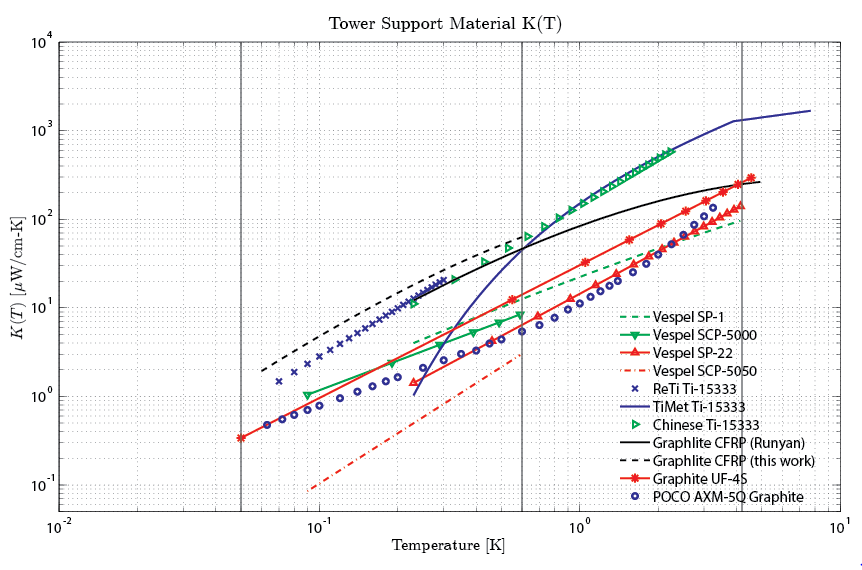
\includegraphics[width = \textwidth]{C:/Users/Niko/Documents/LaTex/Nick_K_Thesis/CH3_figs/Tower_standoff_K.png}
\caption{Thermal conductivity of candidate tower thermal stand-off materials. These data were collected from multiple papers: Vespel SCP-5000, Vespel SCP-5050, ReTi Ti 15-3-3-3, and Graphlite CFRP - This work ; Vespel SP-1, Vespel SP-22, and Graphlite CFRP - \cite{run} ; TiMet Ti 15-3-3-3 - \cite{wik} ; Chinese Ti 15-3-3-3 - \cite{Run_ti153} ;  UF-4S Graphite - \cite{lem} ; AXM-5Q Graphite - \cite{woo:gr}.}
\end{figure}

We are concerned with thermal conductivities in the temperature range $T \in [0.01,5]$ as this is the span of the temperatures for the tower stages (including non-ideal temperatures). We see that there are numerous samples whose thermal conductivity is below UF-4S graphite for this range; these materials -- Vespel SP-22, SP-1, SCP-5050, SCP-5000, POCO AXM-5Q graphite, and for lower ranges, TiMetal Ti 15-3-3-3. Other materials -- such as Graphlite -- have a higher thermal conductivity, but are still considered for other compensating properties, such as strength, which will be discussed in the following sections. Note that none of our thermal conductivity data extends to the lowest two stages -- the Cold Plate (50mK) and the Mixing Chamber (10mK). This makes predicting performance at this stage transition (50mK - 10mK) difficult. We will have to address this carefully, typically with fixed exponent extrapolation.



\section{Radioactivity}

The dark matter particles that the CDMS experiment is searching for are a form of radiation; this means that our detectors are extremely sensitive radiation detectors. Our experiment takes extensive measures to ensure that any external sources of background radiation are minimized, as described in section 1.5.1. However, all the passive and active shielding in the world won't help if the materials within the shielding (such as the tower materials) are radioactive. Since the tower thermal stand-offs contribute non-negligibly to the mass of the tower, the radioactivity of candidate materials is of fundamental importance in establishing an effective experiment. To test for the presence of radioactive isotopes in our materials, we sent them to a test facility in Soudan, Minnesota for screening. The measurement process and results of screenings are described below. The results are presented in Table 4.2, which gives the total activity for transmutational processes (e.g. $\alpha$-decay, $\beta$-decay, Spontaneous Fission) for the isotopes Th-232, U-238, Co-60, K-40, and Cs-137.

\subsection{Secular Equilibrium}

\begin{wrapfigure}{r}{6.8cm}
\centering
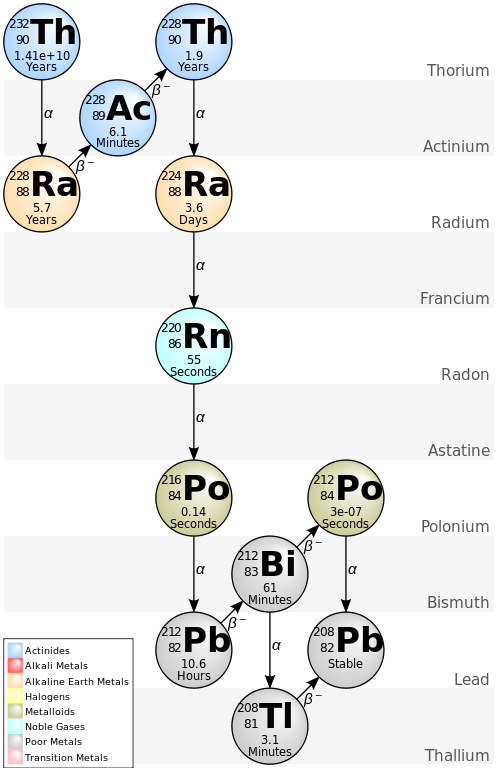
\includegraphics[width=.32\textwidth]{C:/Users/Niko/Documents/LaTex/Nick_K_Thesis/CH3_figs/Th232_chain.png}
\caption{One decay chain for Th-232, which ends with the stable isotope Pb-208. The long half-life of Th-232 allows one to assume a secular equilibrium for undisturbed samples with Th-232 contamination. The figure shows the half-lives of the isotopes, as well as their method of decay.}
\end{wrapfigure}

Secular equilibrium is the assumption of a near-equilibrium in the decay chain of a radioisotope. It assumes that the decay rates for all daughters in a given decay chain are equal. It is a crucial concept for the following sections, so will briefly be explained here.

The validity of assuming secular equilibrium comes from the length of the half-lives of parent isotopes under examination. The isotopes screened for in Gopher are all very stable radioisotopes, with half lives on par with the age of the universe. This is crucial, as it means that over a given period of time, the decay rates of the isotopes are nearly constant (because the total population of the parent isotope doesn't change noticeably over time periods which are small compared to its half-life). Consider the decay chain for Th-232, shown in Figure 4.2. As Th-232 decays, Ra-228 particles are created at a constant rate. The Ra-228 particles will subsequently decay into Ac-228 particles, at a rate determined by their half-life. The population of Ra-228 will increase until its decay rate is equal to the constant creation rate. This will occur for Ac-228, Th-228, and all other daughters in the decay chain, with final decay rates being set by the decay rate of the initial Th-232 parent. Therefore, secular equilibrium yields an expected abundance for each daughter isotope in the decay chain -- based on their relative half-lives -- as well as identical decay rates for all daughters in the chain.

The assumption of secular equilibrium can be invalidated if the half-lives of the parent isotopes are not sufficiently long, or through processes which remove or add isotope populations and break secular equilibrium, such as refining. However, the assumption of secular equilibrium is often very useful in the analysis of radioactive contaminants.


\subsection{Measuring Radioactivity}
To measure the radioactivity of thermal stand-off candidates, we sent them to an underground facility in Soudan, Minnesota. This facility possesses a high-purity germanium detector, called Gopher, which is used as a gamma ray counter. The samples are cleaned thoroughly to remove any contaminants then placed inside a low background environment with the detector, and allowed to remain until sufficient gamma counts are detected for analysis.

\begin{SCfigure}[.6][h]
\centering
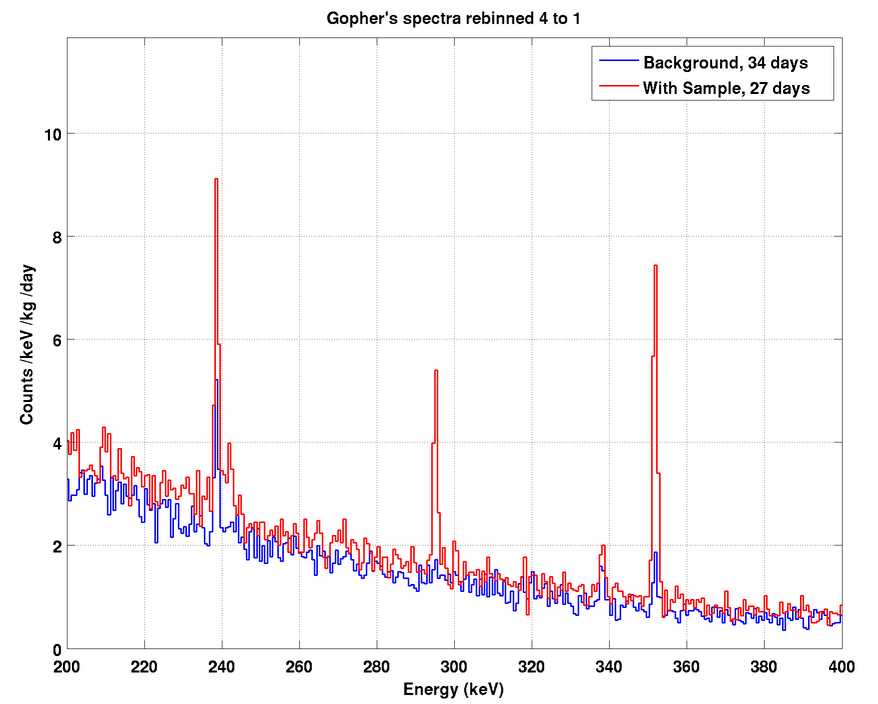
\includegraphics[width = .5\textwidth]{C:/Users/Niko/Documents/LaTex/Nick_K_Thesis/CH3_figs/Gopher_counts_v_background.png}
\caption{Detected gamma spectrum from 200keV - 400keV for a counted Ti 15-3-3-3 foil as obtained from Gopher -- a high purity Ge detector in Soudan, Minnesota. Background counts are shown in blue, while the sample spectrum peaks are clearly visible in red above the background. The 295keV Pb-214 line, for example, is clearly visible in the middle of the plot. Plot from \cite{GopherTi15333}.}
\end{SCfigure}

\subsubsection{Counting}
The counting process itself relies on low backgrounds which are precisely characterized. Once a background spectrum is obtained, the sample is placed in the detection chamber and counted until a reliable activity above background is obtained. Figure 4.2 shows such a spectrum for a gamma energy of 200keV to 400keV, in which the sample activity (shown in red) is clearly visible above the background activity (in blue). Background is then subtracted away, and the count rate of prominent lines for isotopes of interest are determined. The long-lived isotopes currently screened for in Gopher are Th-232, U-238, Co-60, K-40, and Cs-137. An example of a prominent daughter isotope line -- the 295keV Pb-214 line from U-238 decay -- is shown in the center of Figure 4.2. Finding the gamma rate for specific daughter isotopes, however, is not enough to determine activity of the parent isotopes. Simulation is required for finding the total activity of the sample.

\subsubsection{GEANT4 Monte Carlo Simulation}
While radioactive screening with Gopher gives us the gamma emission rate for various radioisotopes, we are actually concerned with the decay rate of the isotopes in the sample (which is the rate of isotope disintegration into another isotope). To convert to true activity of the sample, the peak detection ratio must be determined for each line. This is accomplished by GEANT4 Monte Carlo simulation of the sample.

GEANT4 (GEometry ANd Tracking) is a set of scripts which, through Monte Carlo methods, simulates the passage of particles through matter. This simulation takes into account many factors such as the geometry of the sample, position with respect to the detector, gamma intensity for various decay methods, and composition of the sample to estimate the peak detection ratio, defined as [number of counts observed for a line]/[number of MC-simulated events for a line] which simply determines what fraction of total events are detected as gammas in the detector. The Monte Carlo is run for each isotope in a chain by homogenously distributing that isotope through the sample. From here, given the considerations above, the peak detection ratio of detections/events for each isotope can be determined. Figure 4.3 shows a visualization of this process for Vespel SCP-5050. The right two figures show simulations of particle decay which track the movement/scattering of particles from the top and side perspective, respectively, while the leftmost figure shows the sample (dark rods) in the screening chamber with the Ge detector (silver cylinder in back).

\begin{figure}[h]
\centering
\begin{minipage}{.34\textwidth}
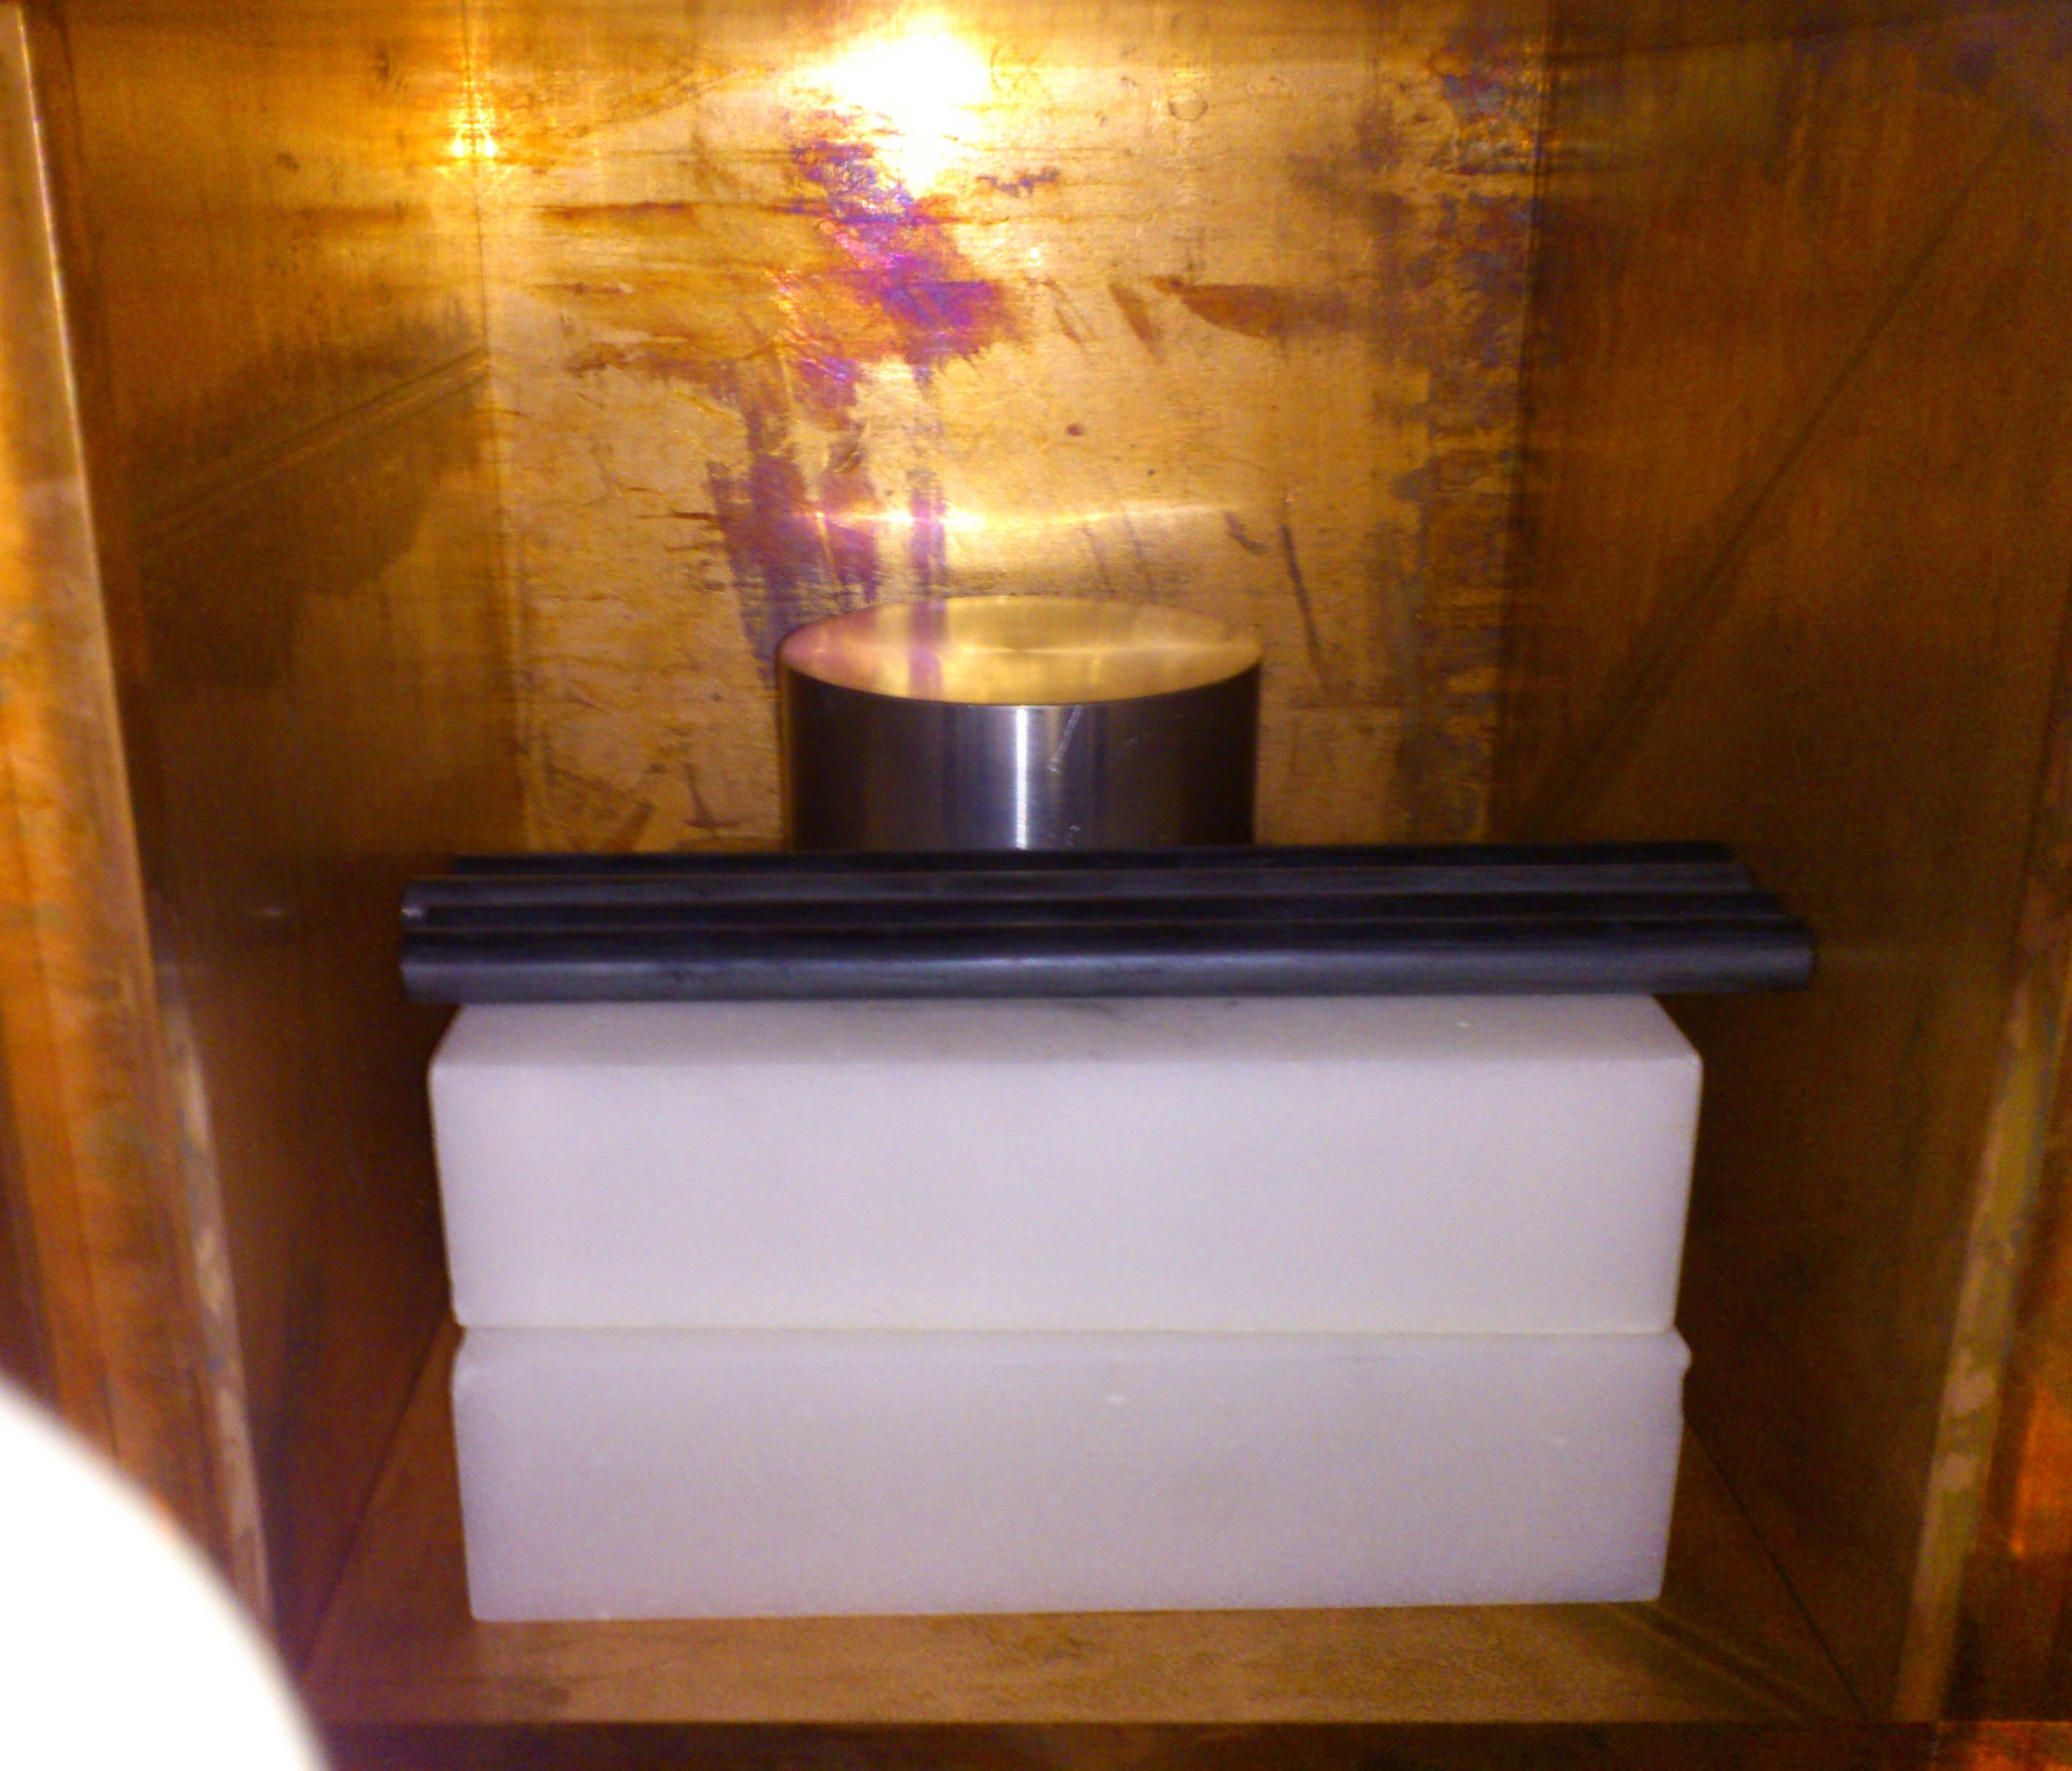
\includegraphics[width = \textwidth]{C:/Users/Niko/Documents/LaTex/Nick_K_Thesis/CH3_figs/VespelSCP5050_In_Gopher.jpg}
\end{minipage}
\begin{minipage}{.3\textwidth}
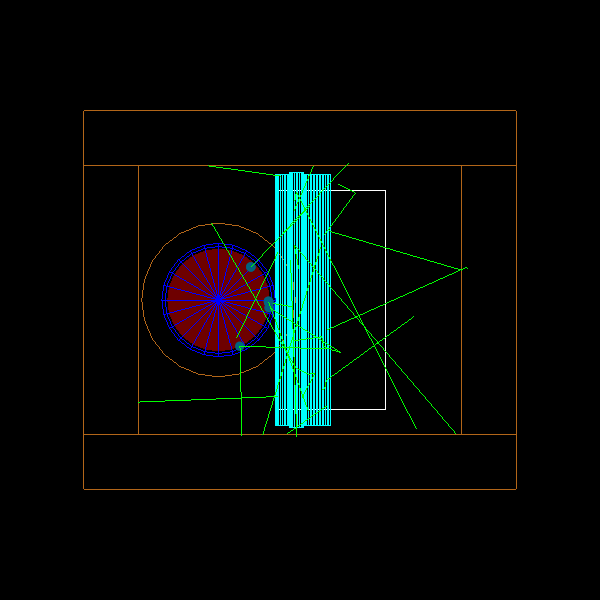
\includegraphics[width = \textwidth]{C:/Users/Niko/Documents/LaTex/Nick_K_Thesis/CH3_figs/VespelSCP5050_Top_Hits.png}
\end{minipage}
\begin{minipage}{.3\textwidth}
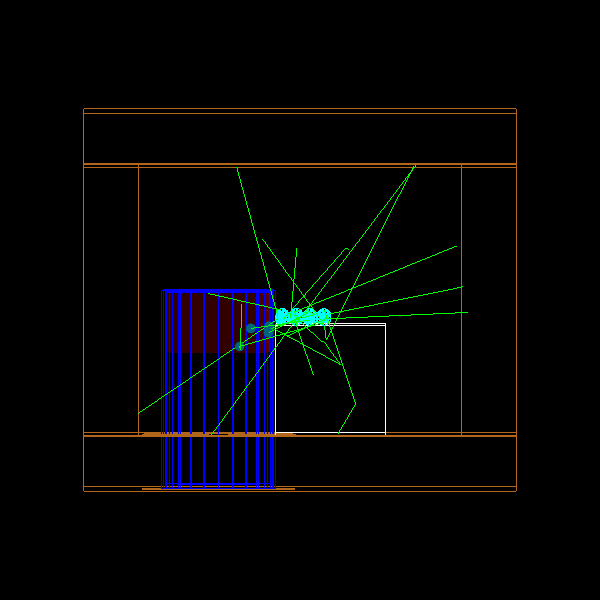
\includegraphics[width = \textwidth]{C:/Users/Niko/Documents/LaTex/Nick_K_Thesis/CH3_figs/VespelSCP5050_Side_Hits.png}
\end{minipage}
\caption{Vespel SCP-5050 sample in Gopher. The left figure shows the sample placement in the detection chamber, with PE. The middle and right figure show the GEANT4-MC simulations from the top and side perspectives, which track particle movement through the sample, chamber, and detector. Images from \cite{GopherSCP5050}.}
\end{figure}

\subsubsection{Determining Total Activity for Each Line}

Once the peak detection ratio is calculated for each line, the gamma rates can be converted to contamination. Then, assuming secular equilibrium, we know that the contamination (decays/second) should be equal for each isotope in a given decay chain. Due to the finite accuracy of statistics, this may not always be true, so a weighted average of the prominent daughter isotope contaminations is performed, which then gives the total contamination of the five parent isotopes screened for. Figure 4.5 shows the calculated contamination for various daughter isotopes of Th-232, U-238, Cs-137, Co-60, and K-40. These are the daughter contaminations that were used in Vespel SCP-5050 to determine parent isotope contamination.

\begin{SCfigure}[.5][h]
\centering
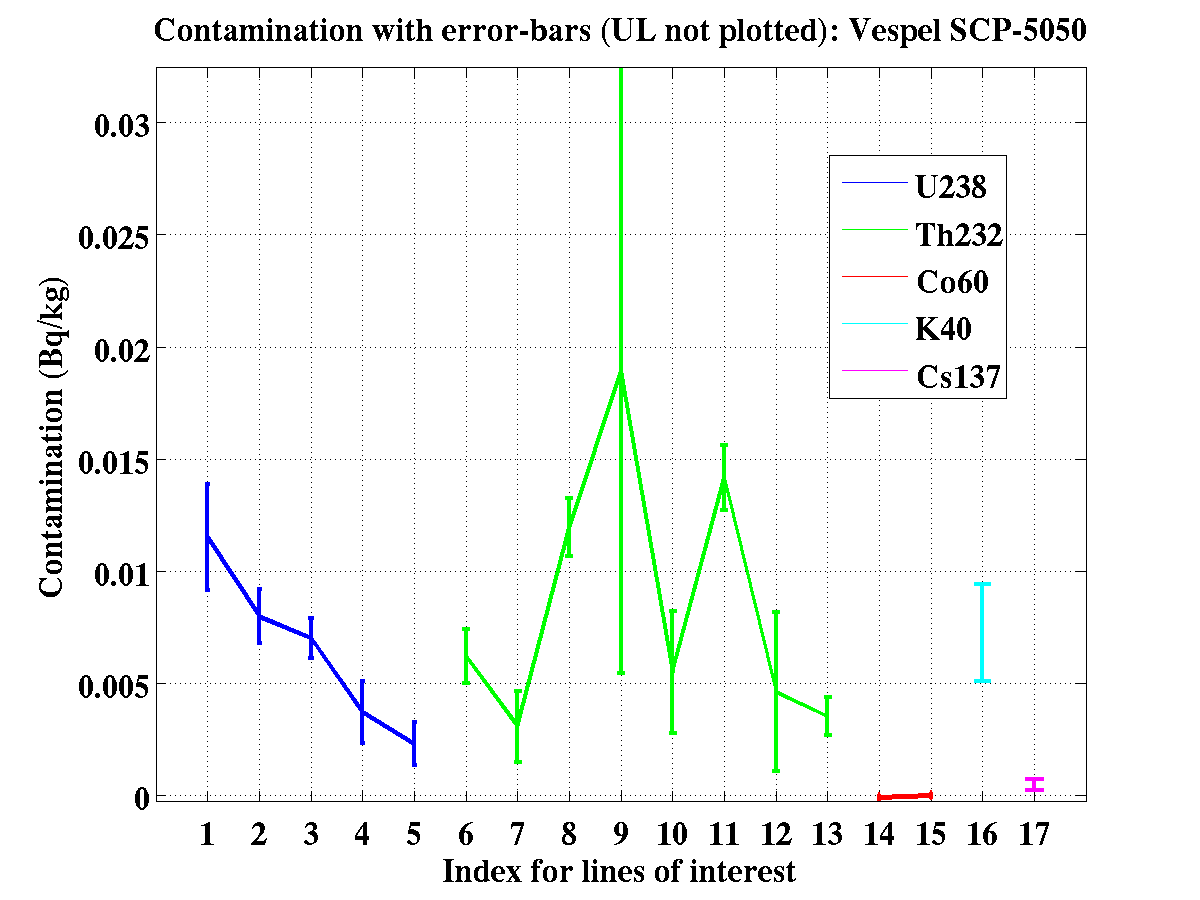
\includegraphics[width = .55\textwidth]{C:/Users/Niko/Documents/LaTex/Nick_K_Thesis/CH3_figs/SCP5050_contamination.png}
\caption{Calculated contamination of daughter isotopes used to determine contamination of each parent isotope. The indices represent specific lines for daughter isotopes in decay chains. 1-5 are for daughters of U-238, 6-13 are for daughters of Th-232, 14-15 are for Co-60, 16 is for K-40, and 17 is for Cs-137. Figure from \cite{GopherSCP5050}. }
\end{SCfigure}

\subsubsection{Results}

The results of Gopher screenings are shown in Figure 4.2 with contamination levels for different isotopes given in milliBecquerels/kilogram. The graphite currently in use, UF-4S (old), shows almost no contamination with $<2$ mBq/kg of U-238. However, new samples of the same material show much higher contamination levels, $\sim 50$mBq/kg of Th-232, despite purification. This irreproducibility in radiopurity levels between graphite batches has been a problem before; when originally purchased, one batch of UF-4S showed too much contamination to use. 2020 graphite is from the same company as UF-4S (Mersen) and shows similar levels of contamination as the new UF-4S stock. These levels are likely higher than what our experiment can tolerate. The next three graphite grades are from Poco Graphite: ACF-10Q, AXM-5Q, and ZXF-5Q. They are all industrial graphite grades, as compared with UF-4S and 2020, which are nuclear grade. This is apparent in their significantly higher contamination levels. The next counted sample, AXM-5Q (p) was purified by Mersen, in the process described below. This purification proved to be extremely effective, decreasing activity by a factor of $\sim50$ to acceptable levels. Vespel SP-1 shows low levels of contamination as well, making it an ideal candidate from a radioactivity level perspective. The next sample, Vespel SP-22 shows very high levels of contamination, due its high graphite content, which rule it out as a candidate for the thermal stand-offs. Surprisingly, SP-22's successor, Vespel SCP-5050, shows very promising levels of contamination, which may be acceptable depending on the amount used in the experiment. The next two samples, Ti 15-3-3-3 and Graphlite CFRP, show similar levels of contamination which again, may be acceptable depending on the mass used in the experiment.

\subsubsection{Graphite Purification}
Graphite such as AXM-5Q are of interest in our experiment, and in many experiments, due to their very low thermal conductivity. However, as the results of screening show, they are often contaminated with high levels (by our standards) of radioisotopes. Therefore, the purification processes offered by Mersen and Poco are of great interest. The results are clearly visible in Table 4.2 for AXM-5Q, which saw its activity reduced by a factor of 50 post-purification.

The purification process offered by Mersen reduced impurities from around 1000ppm to $<$1.4ppm for all purified samples (including those from Poco, which were sent to Mersen for purification) \cite{Mersen_conv}. The graphites are placed in an environment of chlorine gas pressurized above 15psi and heated to roughly $2000^{o}C$. In these conditions, the chlorine permeates the material and readily bonds with oxidizable metals to remove them from the sample \cite{Olivier_conv}. This is more effective the thinner/more porous the graphite.

\begin{table}[htb]
\centering
\begin{threeparttable}
\rowcolors{3}{gray!20}{white}
\begin{tabular}{l|rrrrr}
\multirow{2}{*}{\large{Material}} & \multicolumn{5}{c}{Contamination in mBq/kg}\\
& U-238 & Th-232 & Co-60 & K-40 & Cs-137 \\\toprule
UF-4S Graphite (old) & 1.33 $\pm$ 2.18 & - & - & - & -\\
UF-4S Graphite (new, p) & - & 52.03 $\pm$ 3.11 &- & -& - \\
2020 Graphite (p) & 3.89 $\pm$ 0.60 & 79.63 $\pm$ 2.02 &- & 4.10 $\pm$ 1.65 &- \\
ZXF-5Q Graphite (u-p) & 159.73 $\pm$ 4.37 & 218.11 $\pm$ 5.26 & - & - & - \\
ACF-10Q Graphite (u-p) & 406.77 $\pm$ 6.51 & 286.65 $\pm$ 5.73 & -& 35.90 $\pm$ 8.02 &-\\
AXM-5Q Graphite (u-p) & 117.71 $\pm$ 2.39 & 217.13 $\pm$ 3.79 &- & -&-  \\
AXM-5Q Graphite (p) & 0.93 $\pm$ 0.25 & 4.93 $\pm$ 0.70 & -& 0.96 $\pm$ 1.16 & - \\
Vespel SP-1 & -& 5.39 $\pm$ 4.80 & -& -&-  \\
Vespel SP-22 & 48.38 $\pm$ 4.83 & 211.10 $\pm$ 8.99 &- & 7.82 $\pm$ 6.09 &\\
Vespel SCP-5050 & 7.72 $\pm$ 0.69 & 9.95 $\pm$ 0.72 &- & 7.26 $\pm$ 2.18 & 0.48 $\pm$ 0.26 \\
TiMet$^{\circledR}$ Ti 15-3-3-3 & -& 17.20 $\pm$ 3.20 &- &- & - \\
Graphlite$^{\circledR}$ CFRP & 2.79 $\pm$ 0.89 & 0.707 $\pm$ 1.39 &- & 24.00 $\pm$ 4.96 & -\\

\end{tabular}
\caption{Activity of listed parent for each sample. Screened at Gopher, a high purity Ge
gamma counter in Soudan, MN. The two results for UF-4S graphite are from the old stock (currently in use in SuperCDMS Soudan) and new stock, purchased recently. For the graphites, u-p refers to unpurified stock samples, while p refers to those samples which have been purified by the method described in this section.}
\end{threeparttable}
\end{table}

\begin{table}[htb]
\centering
\begin{threeparttable}
\rowcolors{3}{gray!20}{white}
\begin{tabular}{l|ccccc}
\multirow{2}{*}{\large{Material}} & \multicolumn{3}{c}{$\frac{Neutrons}{year \cdot cm^{3}}$}\\
& Sponteneous Fission & ($\alpha$,n)-reactions & Total \\\toprule
CDMS Graphite & 2.1 $\cdot 10^{-4}$ & - & 2.1 $\cdot 10^{-4}$ \\
ZXF-5Q Graphite & - & - & - \\
ACF-10Q Graphite & - & - & - \\
AXM-5Q Graphite & - & - & - \\
Vespel SP-22 & - & - & - \\
Vespel SP-1 & - & - & - \\
Ti 15-3-3-3 & 3.04 $\cdot 10^{-7}$ & 2.09 $\cdot 10^{-6}$ & 2.4 $\cdot 10^{-6}$ \\

\end{tabular}
\caption{Neutron production per year for 1 $cm^{3}$ of material for candidate materials}
\end{threeparttable}
\end{table}

\subsection{Using SOURCES-4C to Predict Neutron Emission Rates}
Neutron background is the largest concern for our detectors as it produces a
nuclear recoil which, along with no charge collection, mimics the expected signal
from WIMPS. In our candidate materials, there are two sources of neutrons:
Spontaneous Fission and ($\alpha$,n)-reactions. The rates at which these occur for each material are determined by two factors: which radioisotopes are present in the material (determined by the Gopher screenings), and the elemental composition of the material. The elements in a material serve as the target materials for the ($\alpha$,n)-reactions, particularly low-Z elements (which have lower Coulomb barriers preventing the $\alpha$-particle from reacting with the nucleus). Therefore, the total activity for each material is not the primary determining factor; in an ideal situation, we would consider candidates based on acceptable neutron emission rates.

To model the neutron emission rate of each material, we used SOURCES-4C, a program
developed by Los Alamos National Laboratory and Texas A\&M University. This
program allows calculation of neutron emission rates through both spontaneous
fission and ($\alpha$,n)-reactions using an extensive library of parameters
such as reaction and stopping cross-sections,product nuclide level branching
fractions, etc.

For our problem, the input parameters for SOURCES-4C were:
\begin{enumerate}
\item Constituent elements in atom fraction
\item Alpha sources in atoms/cc
\item Target materials in atom fraction
\end{enumerate}

To determine the $\alpha$-source contamination in atoms/cc we have to convert
from the total activity values in Table 4.2. To do this, we first find the concentration of the parent isotopes given in the table. This is done by starting with the equation for the time-dependent population of a radioisotope,
\begin{eqnarray}
D(t) & =& D_0\left(\frac{1}{2}\right)^{t/h} \\
\end{eqnarray}
where D(t) is the population at any time t, $D_0$ is the population at t = 0, and h is the half-life of the particle in seconds. Taking the derivative of both sides, we can find the rate of change in population at any t. This gives
\begin{eqnarray}
D'(t) = \frac{ln\left(\frac{1}{2}\right)}{h}D_0\left(\frac{1}{2}\right)^{t/h} = \frac{ln\left(\frac{1}{2}\right)}{h}D_0 \ \ , \ \ t << h
\end{eqnarray}

the simplification on the right side of the equation comes from observing that t is always small when compared to the half-lives of the parent isotopes under consideration, so $(1/2)^{t/h} \sim 1$. To get to atoms/$cm^3$ we convert D'(t) to R (activity in Bq/kg), multiply by material density, $\rho$ (in $kg/cm^3$), and rearrange:

\begin{eqnarray}
D_0 = D = -\frac{R \rho h}{ln\left(\frac{1}{2}\right)}
\end{eqnarray}

where the R for each parent isotope comes from the screening results.

Once we have the contamination of the parent isotope we can then find the
corresponding contamination for all $\alpha$-emitting daughters by assuming secular equilibrium. This allows us to set R equal for all isotopes in a decay chain. Exploiting this equality in equation 4.6, we obtain
\begin{eqnarray}
\frac{D_i}{h_i} = \frac{D_k}{h_k}
\end{eqnarray}
where the subscripts denote different isotopes in secular equilibrium. This says that, in secular equilibrium, the ratio of isotopes present in a given decay chain depends only on the ratio of those isotopes' half-lives. This can be applied to find the amount of each daughter isotope from the parent isotope in a chain with,
\begin{eqnarray}
D_{d} = D_{p}\frac{h_{d}}{h_{p}}
\end{eqnarray}

where the subscripts d and p refer to daughter and parent, respectively.

Finally, we input the elements in the material under consideration which act as targets for the $(\alpha,n)$ interactions. Doing this, we can obtain the total predicted neutron production per volume of the material under consideration. Table 4.2 presents some preliminary results for predicted neutron emission per cm$^3$ of material for CDMS Graphite (grade UF-4S) and TiMetal Ti 15-3-3-3. This table, in conjunction with the dimension optimizations presented in section 4.6, can predict total expected neutron emission from the thermal stand-offs for the experiment.

If we find that the expected neutron emission approaches acceptable limits using the simple process mentioned above -- where any neutron emitted is assumed to hit the detector -- we can refine our model to account for parameters such as the solid angle subtended by the detectors from the thermal stand-offs.


\section{Thermo-Mechanical Properties}

The tower thermal stand-offs are a structural component of the tower, so the physical and mechanical properties of the materials are naturally an important factor in choosing suitable candidates. In Table 4.4 \& 4.5 I examine some of the physical quantities of interest for possible thermal stand-offs materials. These numbers characterize the strength and dimensional stability of the materials. Dimensional stability is required to ensure the correct operation of our rigid vacuum coaxes; if the tower flexes too much during handling, the vacuum coaxes could be put under too much tension and snap. Similarly, during fridge operation, a CTE which is too high could cause the vacuum coaxes too go slack and short to their shielding; a CTE which is too low could cause too much tension and plastically deform the lines. The different strength parameters are crucial in telling us how little of the material we can safely use in creating a sufficiently strong support. Since radioactivity levels and thermal power conducted depend on volume and cross-section of the material, respectively, by minimizing material use we also minimize radioactivity and thermal loads to the dilution fridge stages.

\begin{table}[htb]%THERMOPHYSICAL PROPERTIES
\begin{threeparttable}
\rowcolors{3}{gray!20}{white}
\begin{tabular}{lcccccc}
\toprule
\textbf{Material} & $\rho$ ($g/cm^3$) & $\nu$ & $\sigma_{t}$ (MPa) & $\sigma_{c}$ (MPa)
& $\sigma_{f}$ (MPa) & CTE $(\mu m/(m\cdot C^o))$ \\
\midrule
 UF-4S Graphite & 1.76  & 0.2 & 18.4$^{\dag}$ & 55.2$^{\dag}$ & 27.6 & 1.8-2.9 \\
 2020 Graphite & 1.77 & 0.15 & 29 & 98 & 45 & 4.3 \\
 POCO AXM-5Q & 1.73 & 0.3$^{*}$ & 48 & 124 & 69 & 7.8 \\
 Ti 15-3-3-3 & 4.71 & 0.36 & 1117 & 1052 & - & 8.45 \\
 Ti 21S & 4.93 & 0.34 & 958 & 1108 & - & 7.07 \\
 Vespel SP-1 & 1.43 & 0.41 & 86.2 & 133 & 110 & 54.0$^{\ddag}$ \\
 Vespel SCP-5000 & 1.46 & - & 163 & 640 & 254 & 45.0 \\
 Vespel SP-22 & 1.65 & - & 51.7 & 112 & 89.6 & 38.0 \\
 Vespel SCP-5050 & 1.76 & 0.22 & 72 & 219 & 130 & 29.0 \\
 Graphlite CF Rod & 1.55 & -  & 2340 & 1900 & - & - \\
 \bottomrule
\end{tabular}
\caption{Some thermo-mechanical properties of candidate materials. $\nu$ is the Poisson's ratio for the material, while $\sigma_{t}$,$\sigma_{c}$, and $\sigma_{f}$ are tensile, compressive, and flexural strengths for the material, respectively. CTE is the linear coefficient of thermal expansion, given at room temperature for all materials. The properties given for Ti 15-3-3-3 and Ti 21s are lower limits for solution-treated, age-hardened samples. These numbers can be higher or lower depending on the specific heat treatment. All Vespel data are for Isostatically-formed parts. All Graphlite CFRP data is along the fiber axis. \dag - Compressive and tensile strengths were derived from the flexural strength, using an apparent trend in graphite materials where tensile $\approx$ 2/3 flexural and compressive $\approx$ twice flexural. * - A poisson ratio of 0.3 is typical for many graphites. \ddag - DuPont data for SP-1 gives a CTE of 45 $(\mu m/(m\cdot C^o))$ for -62$^{o}$C - 23$^{o}$C, whereas the number given in the table is for 23$^{o}$C and above. Data for Ti 15-3-3-3 and Ti 21s from \cite{Nyakana2005} and \cite{Johnson1996}. All other data from manufacturer websites or datasheets.}
\end{threeparttable}
\end{table}

\begin{table}[htb]
\centering
\begin{threeparttable}
\rowcolors{3}{gray!20}{white}
\begin{tabular}{lccc}
\toprule
\textbf{Material} & $E_{T}$ (GPa) & $E_{C}$ (GPa) & G (GPa) \\
\midrule
 UF-4S Graphite & 7.2 & - & 4.48 \\
 2020 Graphite & 9.2 & - & 4.1 \\
 POCO AXM-5Q & 10.5 & - & 4$^{\ddag}$ \\
 Ti 15-3-3-3 & 105 & - & 39.5$^{\ddag}$ \\
 Ti 21S & 103 & 114 & 38.7$^{\ddag}$ \\
 Vespel SP-1 & 2.3$^{*}$ & 2.41 & - \\
 Vespel SCP-5000 & 3.99 & 9.06 & 1.41$^{\ddag}$\\
 Vespel SP-22 & 3.3$^{*}$ & 3.28 & - \\
 Vespel SCP-5050 & 8.93 & 3.00 & 3.66$^{\ddag}$\\
 Graphlite CF Rod & 134 & 131 & - \\
 \bottomrule
\end{tabular}
\caption{Continuation of Table 4.4 for thermo-mechanical properties. Different moduli are given for each material: $E_{T}$ is the Young's Modulus, $E_{C}$ is the compressive modulus, and G is the shear modulus. \ddag - Indicates that data on the shear modulus, G, was unavailable; instead, the formula for homogenous and isotropic materials was used, in which $G = E_{T}/(2(1 + \nu))$. * - Data from material properties table published by Oblicos-96, Ltd. (www.oblicos.com). Other references are the same as in Table 4.4. }
\end{threeparttable}
\end{table}

One of the most noticeable aspects of Tables 4.4 \& 4.5 is the wide distribution of structural properties for materials. As with any other qualification discussed in this chapter, some candidates are clearly better suited mechanically; however, this simply reflects the wide array of parameters which must be satisfied, and that different materials were chosen for different particular merits. Below I summarize the interesting results from the tables:
\begin{itemize}
\item UF-4S Graphite (used as a thermal stand-off in SuperCDMS Soudan) has lower strengths than every other material including AXM-5Q,
another graphite. It also has the lowest CTE, which made it well suited as a thermal stand-off in the current towers, where small stage separations demanded minimal contractions to prevent thermal shorts between stages.
\item The two Ti alloys from TiMetal, Ti15-3-3-3 and Ti21s, offer some of the highest strengths of the candidates coupled with low CTEs and high elastic moduli, making them strong candidates.
\item The Vespel SCP series compounds outperform their SP counterparts in nearly every regard. Their strengths show an increase of between 50\% - 400\%, with increased elastic moduli, and decreased coefficients of thermal contraction.
\item Vespel SCP-5000 still has a fairly high CTE -- 45 ppm/C at room temperature. The number below room temperature is likely lower, however, if SCP-5000 follows the same trend as SP-1; this trend gives a CTE for SP-1 of 54ppm/C at room temperature and above, which drops to 45ppm/C from -62$^{o}$C - 23$^{o}$C.
\item Graphlite CFRP offers exceptionally high strength as well as dimensional stability, which suggests that we could safely use very little of the material in order to minimize radioactivity and heat loads.
\end{itemize}

From here, we can now develop models which examine the interplay of properties for these materials.


\section{Thermal Contraction}

The thermal contraction of our tower stand-offs is constrained by the rigid vacuum NbTi coaxes, as described in chapter 2. We must ensure that these coaxes do not experience excessive strain and that they do not go slack during cooldown, which could short them to their copper housing. This is the only constraint, as the new SNOLab tower will feature an open face design, eliminating the 0.03" copper-copper stage separation, along with the need to preserve such a small separation during cooldown.

\begin{figure}[ht]
\centering
\subfloat[Simplified SNOLab tower used to calculate expected thermal contraction behavior of tower components. All stand-off lengths and NbTi coax lengths are assumed to be 2", making the analysis identical for all tower stages.]{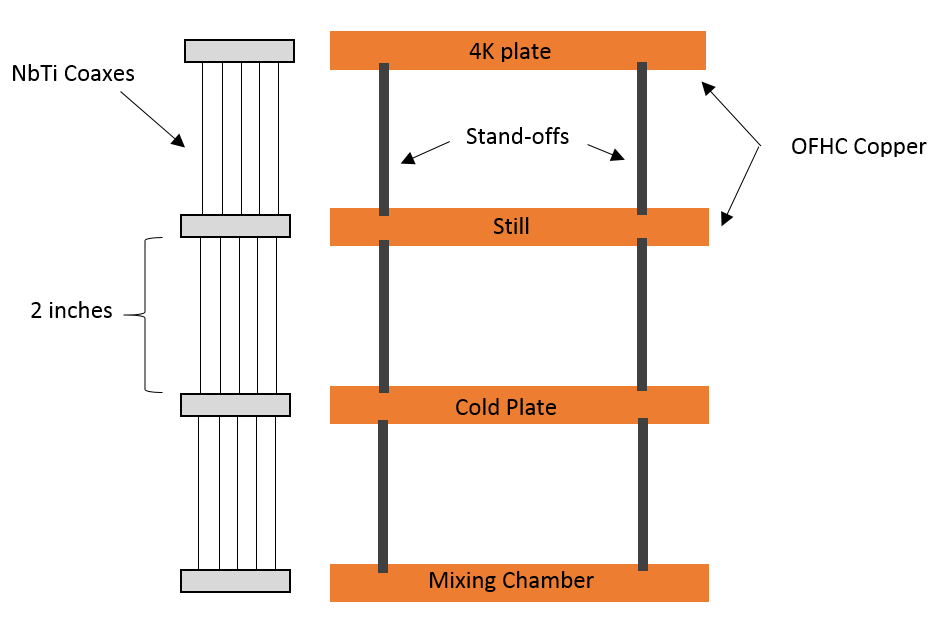
\includegraphics[width = .5\textwidth]{C:/Users/Niko/Documents/LaTex/Nick_K_Thesis/CH3_figs/SNOLab_tower_coax_stress.png}}
\qquad
\subfloat[Model for deflection of NbTi coaxes, where any slack is efficiently translated into a deflection. L is the distance between the coax heat-sinks, and $L_eq$ is the equilibrium length of the NbTi wires at 4K. A deflection $\geq$ 0.021" means that the wires will short to their housing]{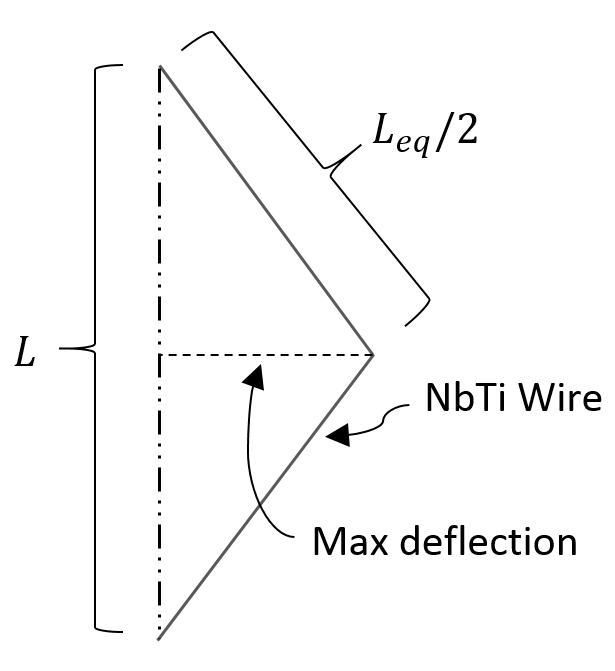
\includegraphics[width = .33\textwidth]{C:/Users/Niko/Documents/LaTex/Nick_K_Thesis/CH3_figs/NbTi_deflection.png}}
\caption{SNOLab model used to determine the strain in the NbTi wires (a), and the slack formed (b) during cooldown.}
\end{figure}

The model used for the SNOLab towers, shown in Figure 4.6a, is simple: it assumes stand-off lengths and vacuum coax lengths are all 2", and considers only the NbTi and stand-off contraction, without considering the CFRP support struts for the coaxes. Much of the analysis follows a previous analysis performed for the Soudan towers, which can be read in greater detail in Appendix A.

\subsection{Strain}
Our goal is to find the strain on the vacuum coax wires during operation of our fridge. This strain can be positive or negative, where a negative strain represents the wires going slack. To find the strain, we use the formula
\begin{eqnarray}
Strain = \frac{L - L_{eq}}{L_{eq}}
\end{eqnarray}
where $L$ is the length of the wires at operating temperature, while $L_{eq}$ is the equilibrium length of the wires at that same temperature (under no strain). In our simple model, L is given at 4K by
\begin{eqnarray}
L = L_{NbTi} - |\Delta L_{stand-off}|
\end{eqnarray}
where $L_{NbTi}$ is the length of the wires at 300K, and $\Delta L_{stand-off}$ is the contraction of the stand-off from 300K to 4K \footnotemark. At the same time, $L_{eq}$ is given by
\begin{eqnarray}
L_{eq \ 300K} & = & L_{NbTi} \cdot (1 - 0.0107) \\
L_{eq} & = & (L_{eq \ 300K})\cdot\left(1 - \left|\frac{\Delta L_{NbTi}}{L_{NbTi}}\right|\right)
\end{eqnarray}
where $L_{NbTi}$ is the actual length of the NbTi wires at 300K, $L_{eq \ 300K}$ and $L_{eq}$ are the equilibrium lengths at 300K and 4K respectively, $\Delta L_{NbTi}/L_{NbTi}$ is the fractional contraction of the wires from 300K to 4K, and the 0.0107 term accounts for the fact that the wires are strained to 1.07\% during fabrication. The fractional contraction of the NbTi wires was calculated from A.1, while the total contraction of various stand-off materials is given by
\begin{eqnarray}
\Delta L = (CTE)(L_{stand-off})(\Delta T)
\end{eqnarray}
where $\Delta L$ is the length change of the stand-off, CTE is the coefficient of thermal contraction -- given by Table 4.4 for various materials, $L_{stand-off}$ is the 300K length of the stand-off, and $\Delta T$ is the total temperature change of the stand-off.

\footnotetext{The thermal contraction formula for NbTi only extended down to 4K. Since the contraction from 4K to $<$1K is negligible compared to the contraction from 300K to 4K, it was ignored.}

The above method was applied to our simple model, producing the upper plot in Figure 4.7. This gives the strain in the NbTi wires at 4K as a function of CTE for stand-off materials. We see that on the lower end, the strain doesn't exceed 1.2\% -- only slightly higher than fabrication strain, and within acceptable limits, according to Figure A.3. On the upper end, the wires experience a "negative strain", which means they have gone slack. This is investigated below

\begin{figure}[ht]
\centering
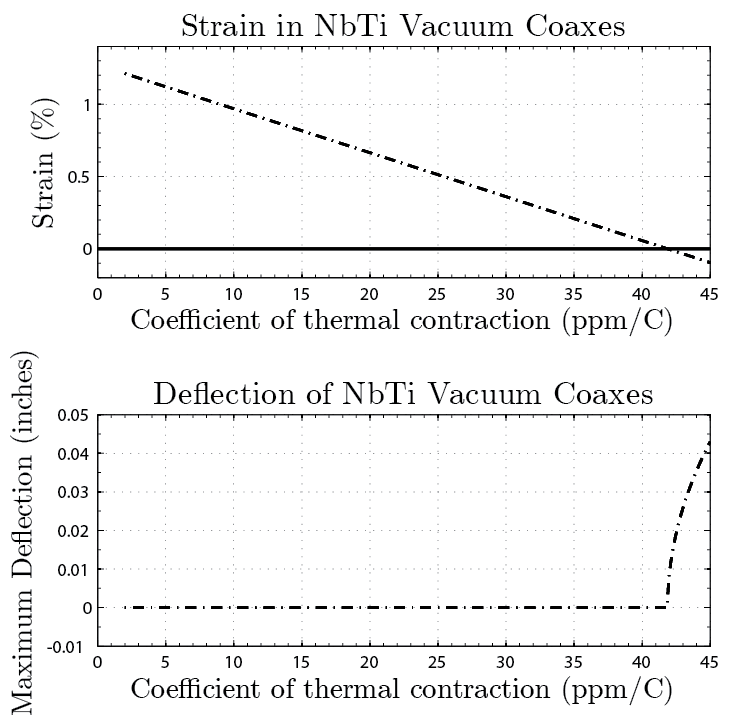
\includegraphics[width = .6\textwidth]{C:/Users/Niko/Documents/LaTex/Nick_K_Thesis/CH3_figs/Coax_strain.png}
\caption{}
\end{figure}

\subsection{Determining Slack in Wires}

The NbTi wires in our vacuum coax lines are suspended and centered in copper grooves which act as shielding during operation. Any slack in the wires could result in a short to these copper grooves, therefore we must determine if the slack experienced by the wires for various stand-off materials may cause a short.

The copper grooves surrounding the wires are 0.042" wide, which means that a deflection of 0.021" in either direction will cause a short to the housing. The model used to test this is shown in Figure 4.6b. We assume that any slack in the wire is perfectly taken up as a deflection (as if one was pulling the wire to the side). The calculated deflection, using this model, is shown in the lower plot of Figure 4.7 as a function of linear coefficients of thermal contraction for tower stand-off materials.

We see that there is no deflection in the wires until the linear CTE of the stand-off reaches 42ppm/C, which is the point when the strain at 4K reaches 0\%. From here, deflection increases rapidly past the 0.021" maximum allowable. In Table 4.4 we see that Vespel SP-1 and Vespel SCP-5000 are above the 42ppm/C limit. As noted in Table 4.4, however, the CTE of these materials is likely lower than the room temperature value given. The CTE of Vespel SP-1 drops from 54ppm/C for room temperature and above, to 45ppm/C below room temperature. Since Vespel SCP-5000 is similar to SP-1, its room temperature CTE of 45ppm/C would likely drop sufficiently low below room temperature to allow its use as a stand-off. If SCP-5000 was chosen for use in the fridge, however, it would be prudent to verify its low temperature CTE.

\subsection{Candidates Based on Thermal Stability}
Considering the strains and deflections found in Figure 4.7 for the range of CTE's found in our candidates, we conclude that all materials besides Vespel SP-1 should satisfy thermal stability requirements in the SNOLab towers, though the low temperature thermal contraction of Vespel SCP-5000 should be verified if it is chosen as a stand-off material.

\section{Tube Stand-offs}

Now that we have characterized the different candidate materials and examined their suitability, we move to the first proposed design for the thermal stand-offs: a thin-walled tube structure. This is the form of our current stand-offs in SuperCDMS Soudan towers. A thin-walled tube uses little material while providing high strength in a variety of loading conditions, making it an attractive design.

The dimensions of the SuperCDMS Soudan thermal stand-offs were selected arbitrarily, based on what sounded reasonable at the time; therefore, we are not attached to these dimensions. Ideally, the dimensions would be different for each material, designed in such a way as to take advantage of the strengths of each. This dimension optimization would allow us to minimize the use of material, reducing both thermal concerns and radioactivity concerns. This section presents a model developed in collaboration with professor Sanjay Govindjee\footnotemark  of UC Berkeley, which considers four failure modes: shear buckling, bending buckling, normal material failure, and shear material failure. Using this model, we determine how little material can safely be used to withstand both a 145lb. and 290lb. transverse shear load. These results will be used later to compare expected heat loads on various tower stages from our optimized tube dimensions.

\footnotetext{s\underline{~}g@berkeley.edu}

\subsubsection{Loading Conditions}

The load conditions which we wish to design to for the SNOLab towers are not yet defined; therefore, as a first pass, we will consider it sufficient to replicate the strength of the Soudan tower stand-offs, which are able to withstand up almost 145lbs applied as a transverse shear force. This was found through a destructive physical analysis (DPA) of a Soudan tower. The tower was clamped in a bench vise, and the 600mK floor was bolted to the 50mK tabs to support it the 600mK to 50mK tube. This isolated the 10mK floor and the tube attached to it. A strap was hung over the 10mK floor, and loaded to $\sim$145 pounds before the tube failed. The load conditions and tube failure are shown in Figure 4.8. This load can be approximated by a transverse shear load. In addition, we assume that the edges are constrained to a circular shape during loading. Therefore, our model will design stand-offs with "clamped edges" which can support 145 pounds as a transverse shear load.

\begin{figure}[ht]
\centering
\subfloat[]{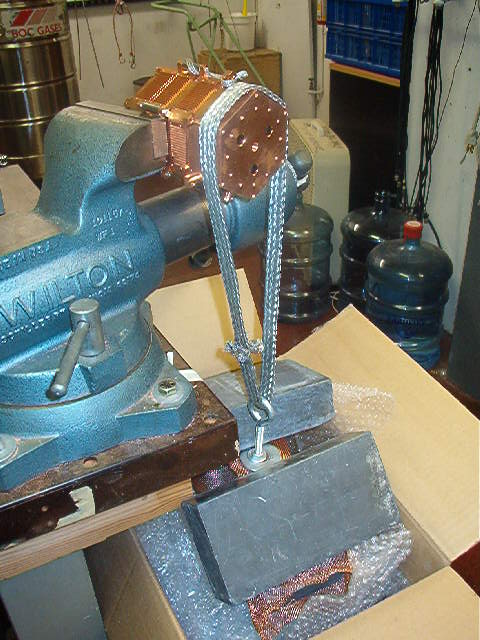
\includegraphics[width = .3\textwidth]{C:/Users/Niko/Documents/LaTex/Nick_K_Thesis/CH3_figs/Tower_loading.jpg}}
\qquad
\subfloat[]{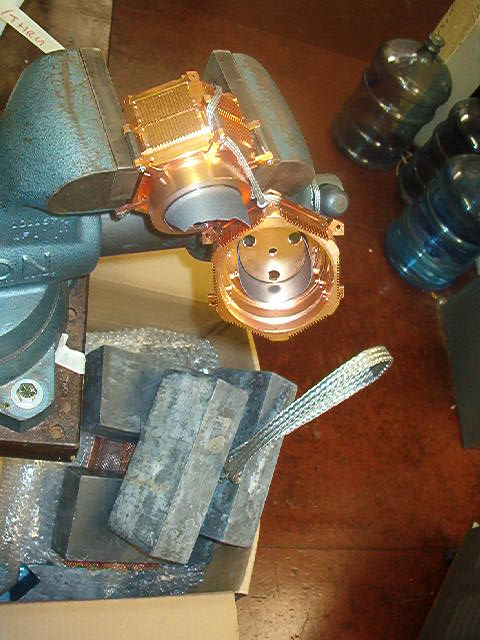
\includegraphics[width = .3\textwidth]{C:/Users/Niko/Documents/LaTex/Nick_K_Thesis/CH3_figs/Tower_break.jpg}}
\caption{Destructive physical analysis of Soudan tower. The 600mK floor was bolted to the 50mK tabs to support it, isolating the 10mK floor and its support. This was then loaded until failure under transverse shear. It failed at $\sim$145 pounds in what appears to be compressive failure.}
\end{figure}

\subsection{Analytical Model for Tube Failure}

Through discussion with Dr. Sanjay Govindjee at UC Berkeley, a model predicting failure loads for different materials/dimensions as well as optimization of Radius/Thickness (a/t) has been developed. The load considered is the same as that used in the Soudan tower DPA (one end fixed, the other subjected to a transverse shear force). This section develops this analytical model as well as its assumptions and limitations. Though an FEA model could be created (and will be to check the results), an analytical model is useful, as it lets one view the entire parameter space and failure trends. Given the prevalence of thin-walled tubes in cryogenic structures, this model has the potential to be of use in broader applications than our own.

Our model considers 4 failure modes:
\begin{itemize}
\item Shear Instability (Buckling)
\item Bending Instability (Buckling)
\item Material Failure from Normal Stresses
\item Material Failure from Shear Stresses
\end{itemize}

A discussion of the formulas for the failure modes considered and their validity follows.

\subsubsection{Tube Geometry}
Cylindrical shell theories depend heavily on certain parameters in the shell, as these permit various simplifications of mechanical models. The tube we will initially try to model is the graphite tube broken in the DPA. The graphite tube tested had nominal dimensions of thickness $t = 0.028$in, radius $a = 0.986$in (to middle surface), and length $L=1.334$in.

For theory, the relevant geometric ratios are
\begin{eqnarray}
\frac{a}{t} = 35.2 \\
\frac{L}{a} = 1.35 \\
Z = \frac{(1-\nu^2)^\frac{1}{2}L^2}{at} = 61.5 \ (\text{for $\nu$ = 0.3})
\end{eqnarray}

where Z is Donnell's parameter. These value imply a fairly thin shell of intermediate length. For dimension optimization, these values may change, and the model may need adjustment. Below are the formulas which are used for Z near this value.

\subsubsection{Shear Instability}

The first failure mode considered is shear instability. Shear instability in will occur when the maximum shear stress in the material, $\tau_{f} = P/\pi at$ exceeds critical torsional stress from a purely torsional load. This torsional stress is given by Yamaki (\cite{Yamaki1984}) as
\begin{eqnarray}
\tau_{b} = \frac{\pi^2E}{12(1-\nu^2)}(1-\nu^2)^{\frac{3}{8}}a_s\left(\frac{t}{a}\right)^{\frac{5}{4}}\left(\frac{a}{L}\right)^{\frac{1}{2}}~~,
\end{eqnarray}

using Donnell's thin shell theory. $a_{s}$ is between 0.81 and 1.04 for $Z \in [50,100]$. As dimensions change, Z could become as high as 400, for which $a_{s}$ is between 0.81 and 0.91. For either case, the lower value of 0.81 is taken to be conservative.

To get critical load ($P_{c}$), set $\tau_{f} = \tau_{b}$ and solve for P:
\begin{eqnarray}
P_{c}^{s} = \frac{\pi^3E}{12(1-\nu^2)^{\frac{5}{8}}}a_{s}\frac{a^{1/4}t^{9/4}}{L^{1/2}}
\end{eqnarray}

To test the validity of Donnell's shell theory in this case we must determine the number of circumferential post-buckling waves present in the shell. This is found from \cite{Yamaki1984},
\begin{eqnarray}
N = \pi(1-\nu^2)^{\frac{1}{8}}b_{s}\left(\frac{a}{L}\right)^{1/2}\left(\frac{a}{t}\right)^{1/4},
\end{eqnarray}
where $\nu$ is poisson's ratio, and $b_{s}$ is related to the boundary conditions, and is between 0.8 to 1.15 for the range of Z values.

This value gives between 3 and 5 waves depending on material/dimensions. Yamaki recommends fully trusting Donnell's shell theory when the wave number is $\geq$5. However, it will only give errors of $\sim$4\% and $\sim$2\% at three and four waves respectively. For current graphite dimensions, we have 5 waves, ensuring accuracy. We must be careful of changing values throughout the optimization process, however.


\subsubsection{Bending Instability}

When dealing with transverse loading, the material may fail due to bending instability. This will occur as local buckling once the maximum compressive stress in the shell wall exceeds some critical value. Approximating the tube as a membrane, the maximum stress in the tube is given by $\sigma_{b} = PL/a^2t\pi$. maximal stress before bending buckling in transverse loading is the same, locally, as for axial compression resulting in axisymmetric buckling. Ba$\check{z}$ant (\cite{Bazant1991}) gives this critical stress a value of,
\begin{eqnarray}
\sigma_{c}=\frac{E}{\sqrt{3(1-\nu^2)}}\frac{t}{a}.
\end{eqnarray}
for Z values greater than 2.85, where E is the modulus of elasticity of the material.

Combining these two conditions gives the critical load for localized bending buckling as:

\begin{eqnarray}
P_{c}^{b} = \frac{E \pi}{\sqrt{3(1-\nu^2)}}\frac{t^2a}{L}
\end{eqnarray}

\subsubsection{Material Failure: Normal Stresses}

The material may fail simply from exceeding its normal stress limit, $\sigma_{f}$ where $\sigma_{f}$ is the minimum of tensile or compressive strength. Then the maximum load for normal material failure ($P_{c}^{mn}$) is:

\begin{eqnarray}
P_{c}^{mn} = \sigma_{f} \pi \frac{a^2t}{L}
\end{eqnarray}


\subsubsection{Material Failure: Shear Stresses}

Failure can also occur from the tube exceeding its shear stress limit, $\tau_{f}$. In ductile materials, $\tau_{f} \approx \sigma_{f}/2 \ \text{or} \ \sigma_{f}/\sqrt{3}$. Brittle material values (such as graphite) can be approximated from $\tau_{f} = \sigma_{t}\sqrt{R/3} $ where $R = \sigma_{c}/\sigma_{t}$ (compressive/tensile) \cite{Ely1965}.

Given $\tau_{f}$, the predicted critical load for shear failure is:
\begin{eqnarray}
P_{c}^{ms} = \tau_{f}\pi at
\end{eqnarray}

\subsubsection{Plotting Failure Curves}

Now that we have defined the failure modes under consideration, we must plot these failure curves for a variety of dimensions to determine the safe parameter space for each material. We do this by rearranging the critical load equations such that we have thickness as a function of radius ($t = f(a)$) assuming that the length (L) of each stage is a fixed value. For shear instability, for instance, we have
\begin{eqnarray}
t = \left(\frac{12(1-\nu^2)^\frac{5}{8}P_{c}^b L^\frac{1}{2}}{\pi^3 E a_s a^{1/4}}\right)^{4/9}
\end{eqnarray}

From here, given the available material properties (Table 4.4 and 4.5) and selecting a desired failure load, we are able to produce a safe parameter-space graph (i.e. one which tells us what dimensions are needed to support a weight up to the failure limit).

To determine the accuracy of our model, we first apply it to the current graphite tubes to try to replicate the results of the DPA (figure 4.8). Using the dimensions of the 50mK-10mK stage tube, and designing for a break strength of 145 lbs (as in the DPA) we obtain Figure 4.9.  The (a,t) combinations which give a failure limit of 145lbs are marked by the dashed green line. Any dimensions to the upper-right of this line are considered safe parameter space (the failure limit is above 145lbs). The model predicts a failure limit of 175lbs for the actual tube dimensions tested. This equates to a $\sim$20\% discrepancy from our model. Given that the strengths input to the model from Table 4.4 and 4.5 are inferred rather than measured (see table notes) this could easily account for the discrepancy. As our model appears to be fairly accurate, we can now apply it to new tower materials.

Next, we use the method described above to plot failure curves for all candidates for each tower stage to determine the safe parameter space. One of the plots is shown in Figure 4.10 for Vespel SCP-5050 and compared to the UF-4S graphite performance for the Still to CP tube (600mK - 50mK). We see that Vespel SCP-5050 offers a large improvement in dimensions over UF-4S graphite; we find this to be true for every other candidate considered for every stage.

\begin{figure}[ht]
\centering
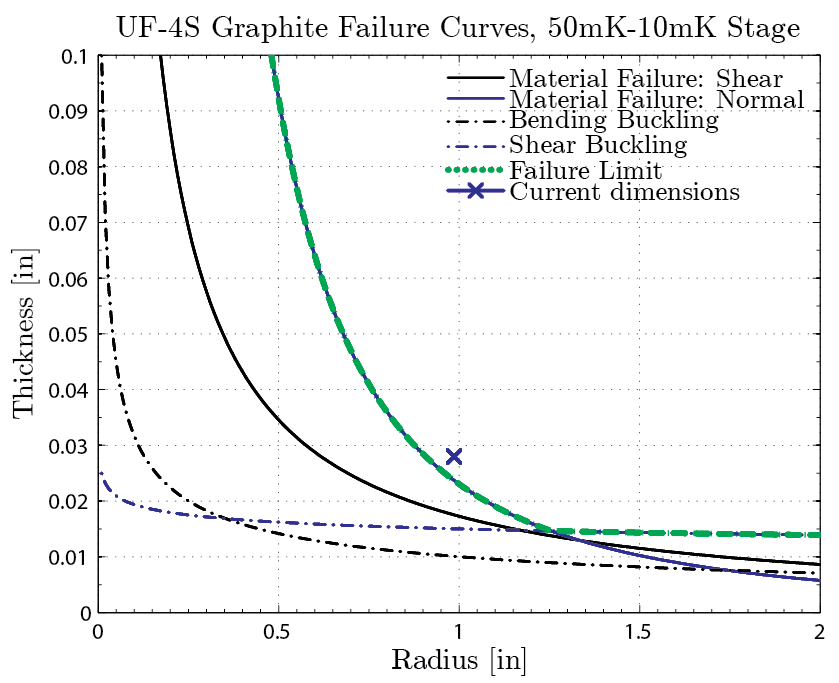
\includegraphics[width = .55\textwidth]{C:/Users/Niko/Documents/LaTex/Nick_K_Thesis/CH3_figs/UF_4S_failure.png}
\caption{Failure curves for UF-4S graphite used in the 50mK-10mK stage SuperCDMS Soudan tower (L = 1.334in). We plot two buckling modes and two material failure modes. In the plot, the highest line at any given radius (a) is the dominating failure mode for that region. This is shown by the green dashed line. Combinations of (a,t) to the upper right of this line represent dimensions whose failure limits are above 145lbs (as set by the DPA); therefore, this region represents the safe parameter space for design. The actual dimensions (t = 0.028", a = 0.986") for the graphite tube are marked by an X. We see that the discrepancy between our model and reality is $\sim$20\%. This may be due to the uncertainty in material properties in Table 4.4 and 4.5.}
\end{figure}

\subsection{Minimizing Radioactivity and Heat Load}


Once the optimal dimension pairs (radius, thickness) are obtained along the failure limit (i.e. green dashed line in Figure 4.9) for each material, we can plot these pairs to determine the dimensions which yield the minimum heat load by minimizing the stand-off cross-section. In fact, by holding tube lengths fixed and minimizing cross-section, we minimize both radioactivity and heat loads simultaneously. This is because radioactivity -- typically proportional to volume -- becomes reduced to a dependence on cross-section once we fix tube lengths; as we already know, heat loads are proportional to material cross-section. Figure 4.11 shows this process for Vespel SCP-5050 and UF-4S Graphite using the dimensions and failure curves from Figure 4.10. We see a very clear minimum heat load for both materials. This method was used for all candidate tube-structure materials to determine minimized expected heat loads for every stage. We present the full results in section 3.8 and compare to hexapod structures.

\begin{figure}[h!]
\centering
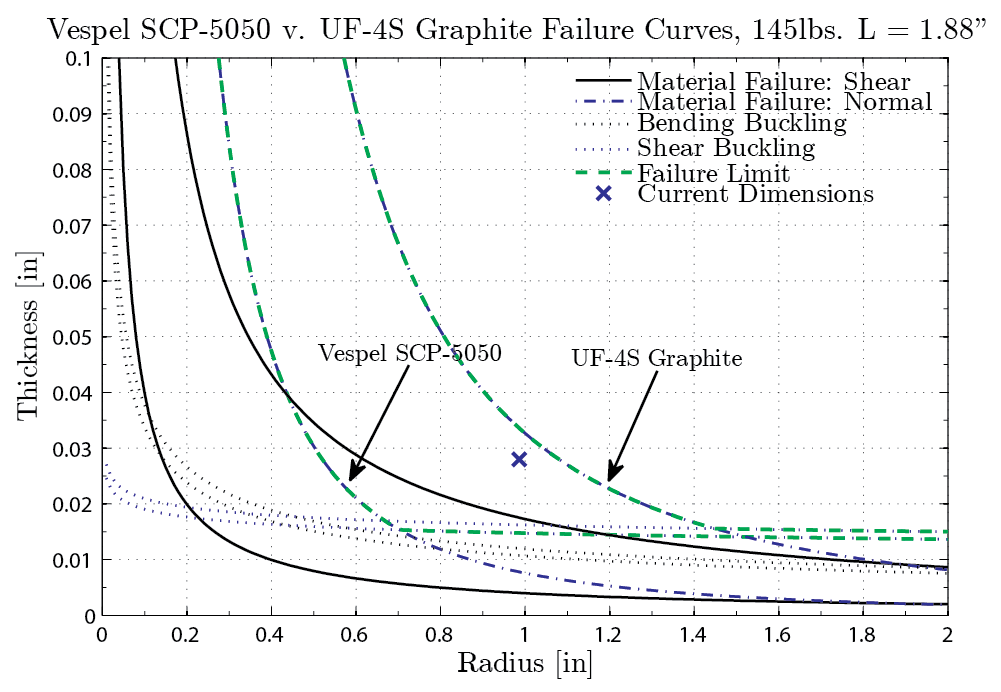
\includegraphics[width = .55\textwidth]{C:/Users/Niko/Documents/LaTex/Nick_K_Thesis/CH3_figs/SCP_5050_graphite_1K_100mK.png}
\caption{Failure curves for Vespel SCP-5050 and UF-4S graphite assuming a stage length of 1.88" and a failure limit of 145lbs. The current dimensions of the graphite are marked with an X. From the plot, we see that Vespel SCP-5050 offers a much better parameter space than UF-4S graphite. As in the previous plot, the (a,t) combinations to the upper right of each green dashed line represent safe parameter space.}
\end{figure}
\begin{figure}[h!]
\centering
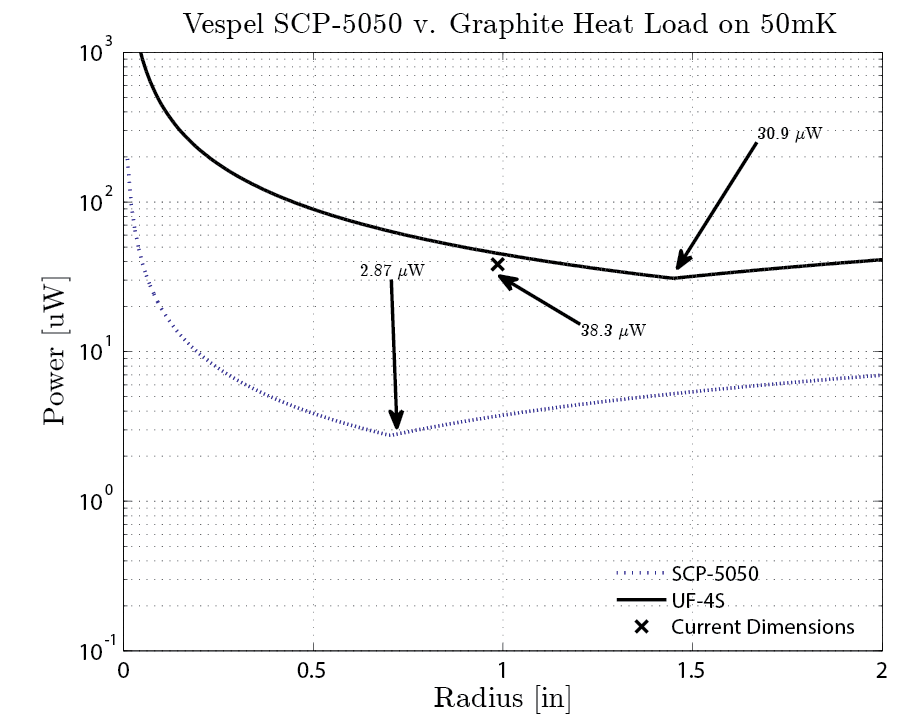
\includegraphics[width = .55\textwidth]{C:/Users/Niko/Documents/LaTex/Nick_K_Thesis/CH3_figs/SCP_5050_graphite_powers.png}
\caption{Plot showing minimization process for heat loads on 50mK stage from 600mK from thermal stand-off tubes (SCP-5050 and UF-4S) for 48 tower experiment, assuming a stage length of 1.88". To get this plot, take the set of optimal (radius,thickness) pairs from the failure curves (green dashed line from Figure 4.9 in this case), and find thermal power conducted for each pair in the set. Though it is not shown in the plot, the optimal thickness is implicitly chosen at each radius. The X denotes heat loads expected from 0.986" radius and 0.028" thickness UF-4S tubes (currently in use in the SuperCDMS Soudan tower). Thermal conductivity data from \cite{lem} for UF-4S, and this work for SCP-5050.}
\end{figure}

\section{Truss Structure Stand-off}

The second proposed design for our tower thermal stand-offs is a truss structure. This design was primarily motivated by the inclusion of Graphlite CFRP (Carbon fiber reinforced plastic) as a candidate material. A truss is a structure consisting of triangular units of straight members; these members meet at nodes which function to permit swiveling of the truss members. An example of a hexapod truss structure is shown in Figure 4.12. Truss structures are a very interesting design for supporting components in cryogenic systems. They use material very efficiently, as they are very open structures whose properties are such that all material in the truss contributes equally to load carrying \cite{Hastings1993}. In addition, their ability to swivel eliminates transfer of moments (bending, etc.) to the members, reducing likelihood of failure.

\begin{figure}[ht]
\centering
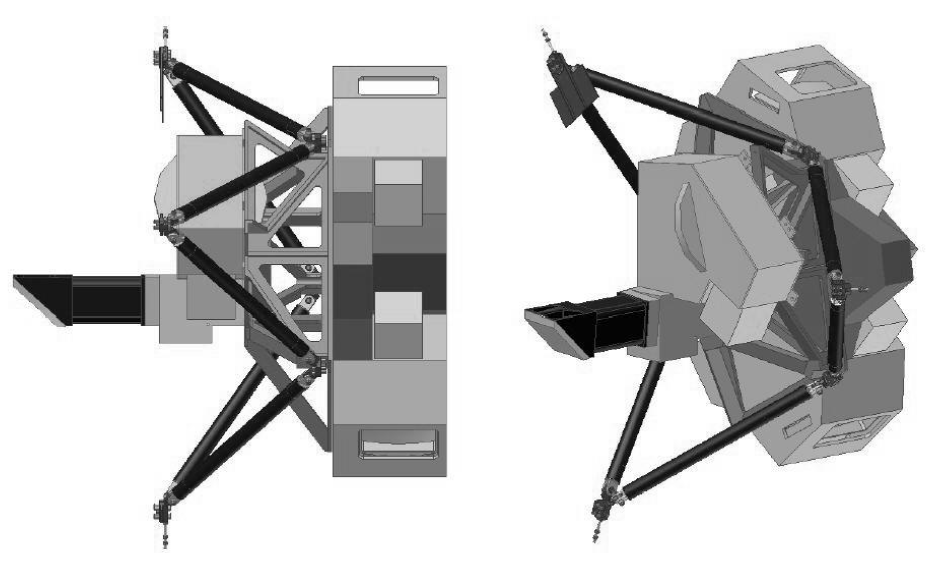
\includegraphics[width = .5\textwidth]{C:/Users/Niko/Documents/LaTex/Nick_K_Thesis/CH3_figs/Hexapod_MIRI.png}
\caption{Hexapod truss structure used to support the MIRI Instrument on the James Webb Space Telescope. The nodes for each member allow motion in two directions to prevent moments from being transferred to the members. Image and description from \cite{Jessen2004}.}
\end{figure}

An analytical model for a truss structure has not been considered yet, but given the interesting properties of trusses, this option will certainly be pursued for candidate thermal stand-off materials. We plan to develop FEA models which will allow us to compare the strength of a hexapod truss to a tube structure. For now, we consider a few novel hexapod structures made from Graphlite CFRP and Ti 15-3-3-3 whose members are angled at $45^{o}$. The expected heat loads from these structures as well as the optimized tube structures are presented in Section 3.8 below.

\section{Expected Heat Loads from Optimized Tube and Novel Truss Designs}

Here we present the expected heat loads and dimensions for our optimized tube structures, as well as some novel hexapod trusses. These thermal loads are calculated assuming 48 towers. The tubes have been designed to a failure limit of 145 and 290 lbs. to allow for a safety factor in their design. The hexapod trusses have not been designed to a specific failure limit. For heat load calculations, all stage lengths are assumed to be 1.88" (seems reasonable). This means that the optimized dimensions for tube structures are identical for each stage. Powers are calculated for ideal temperatures as well as elevated temperatures to observe the thermal stability of all materials.

\begin{table}[!h]
\begin{small}
\resizebox{\textwidth}{!}{%
\rowcolors{3}{gray!20}{white}
\begin{threeparttable}
\begin{tabular}{lccccc}
  \multicolumn{5}{l}{{\Large 4.2K - 600mK: Thermal Stand-off Heat Loads in $\mu$W, 48 Towers}} \\
\toprule
\bf{{\large Material}}& \multicolumn{2}{c}{145lb. Failure} & \multicolumn{2}{c}{290lb. Failure} & Ref.\\
\cmidrule(r){2-5}
& 5K - 1K & 4.2K - 600mK & 5K - 1K & 4.2K - 600mK & \\
Current CDMS Graphite; $(2"\oslash,0.028")$  & 7563 & 4941 & - & - & \cite{lem}\\
Graphlite CF Hexapod; ($0.04" \oslash$ @ $45^{o}$) & 274 & 212 & - & - & \cite{run}\\
Ti 15-3-3-3 Hexapod; ($0.04"$ x $0.06"$ @ $45^{o}$) & 2297-2786 & 1604-1741 & - & - & \cite{wik},\cite{Run_ti153} \\
Vespel SCP-5000; $(0.78"\oslash,0.025")|(0.96"\oslash,0.032")$ & 806 & 568 & 1299 & 915 & -\\
Vespel SCP-5050; $(1.4"\oslash,0.016")|(1.72"\oslash,0.021")$ & 1228 & 748 & 1999 & 1217 & - \\
Vespel SP-1; $(.96"\oslash,0.030")|(1.2"\oslash,0.040")$ & 1649 & 1188 & 2696 & 1942 & \cite{run}\\
POCO-AXM 5Q; $(1.90"\oslash,0.014")|(2.32"\oslash,0.019")$ & 3527 & 1746 & 5740 & 2841 & \cite{woo:gr}\\
Ti 15-3-3-3 $(0.64"\oslash,0.006")|(0.78"\oslash,0.008")$ & 2604-3158 & 1819-1973 & 4224-5123 & 2950-3201 & \cite{wik},\cite{Run_ti153}\\
\bottomrule
\end{tabular}
\end{threeparttable}}
\caption{Heat loads for 4.2K-600mK stage transition including non-ideal fridge temperatures, where power is dissipated on the lower temperature stage in each transition. Tube structures are designed for both 145lb. and 290lb. failure limits. Dimensions are given in (diameter, thickness) pairs for tubes. The left and right set correspond to 145lb. and 290lb. failure limits respectively. The CF Graphlite and Ti 15-3-3-3 hexapods are rods with the given dimensions angled at $45^{o}$. Stage length is taken to be 1.88". The last column gives the reference used for thermal conductivities of each material. Blank references indicate data used from this work. Note that "Current CDMS Graphite" refers to the grade UF-4S graphite used in SuperCDMS Soudan towers.}
\end{small}
\end{table}

\begin{table}[!]
\begin{small}
\resizebox{\textwidth}{!}{%
\rowcolors{3}{gray!20}{white}
\begin{threeparttable}
\begin{tabular}{lccccc}
  \multicolumn{5}{l}{{\Large 600mK - 50mK: Thermal Stand-off Heat Loads in $\mu$W, 48 Towers}} \\
\toprule
\bf{{\large Material}}& \multicolumn{2}{c}{145lb. Failure} & \multicolumn{2}{c}{290lb. Failure} & Ref.\\
\cmidrule(r){2-5}
& 1K - 100mK & 600mK - 50mK & 1K - 100mK & 600mK - 50mK \\
Current CDMS Graphite & 137.3 & 38.3 & - & - & \cite{lem}\\
Graphlite CF Hexapod & 17.1 & 5.73 & - & - & \cite{run}\\
Ti 15-3-3-3 Hexapod & 29.0-34.2 & 4.24-8.45 & - & - & \cite{wik},\cite{Run_ti153} \\
Vespel SCP-5000 & 27.7 & 9.47 & 44.7 & 15.25 & - \\
Vespel SCP-5050 & 12.0 & 2.76 & 19.6 & 4.50 & - \\
Vespel SP-1 & 61.2 & 20.4 & 100.1 & 33.4 & \cite{run} \\
POCO-AXM 5Q & 25.6 & 8.19 & 41.6 & 13.3 & \cite{woo:gr} \\
Ti 15-3-3-3 & 32.9-38.7 & 4.81-9.58 & 53.3-62.9 & 7.8-15.5 & \cite{wik},\cite{Run_ti153}\\
\bottomrule
\end{tabular}
\end{threeparttable}}
\caption{Same as table 4.6, for 600mK - 50mK stage transition.}
\end{small}
\end{table}

\begin{table}[!h]
\begin{small}
\resizebox{\textwidth}{!}{%
\rowcolors{3}{gray!20}{white}
\begin{threeparttable}
\begin{tabular}{lccccc}
  \multicolumn{5}{l}{{\Large 50mK - 10mK: Thermal Stand-off Heat Loads in $\mu$W, 48 Towers}} \\
\toprule
\bf{{\large Material}}& \multicolumn{2}{c}{145lb. Failure} & \multicolumn{2}{c}{290lb. Failure} & Ref.\\
\cmidrule(r){2-5}
& 100mK-40mK & 50mK - 10mK & 100mK - 40mK & 50mK - 10mK \\
Current CDMS Graphite & 3.9\e{-1} & 7.6\e{-2} & - & - & \cite{lem}\\
Graphlite CF Hexapod & 5.54\e{-2} & 1.05\e{-2} & - & - & - \\
Ti 15-3-3-3 Hexapod & 1.23\e{-2}-6.06\e{-2} & 3.5\e{-3}-9.2\e{-3} & - & - & \cite{wik}, - \\
Vespel SCP-5000 & 1.86\e{-1} & 4.86\e{-2} & 2.99\e{-1} & 7.83\e{-2} & - \\
Vespel SCP-5050 & 1.47\e{-2} & 2.1\e{-3} & 2.4\e{-2} & 3.5\e{-3} & - \\
Vespel SP-1 & 3.66\e{-1} & 9.24\e{-2} & 5.99\e{-1} & 1.51\e{-1} & \cite{run} \\
POCO-AXM 5Q & 1.72\e{-1} & 4.65\e{-2} & 2.80\e{-1} & 7.57\e{-2} & \cite{woo:gr} \\
Ti 15-3-3-3 & 1.4\e{-2}-6.87\e{-2} & 4.0\e{-3}-1.04\e{-2} & 2.27\e{-2}-1.11\e{-1} & 6.5\e{-3}-1.69\e{-2} & \cite{wik}, - \\
\bottomrule
\end{tabular}
\end{threeparttable}}
\caption{Same as Table 4.6 for 50mK - 10mK stage transition.}
\end{small}
\end{table}

We see from Tables 4.6, 4.7, and 4.8 that there are numerous competitive options available for our thermal stand-offs. The candidates which seem most promising are described below.

\smallskip

\textbf{4.2K - Still (4.2K - 600mK):} For this transition, a Graphlite CFRP hexapod is the ideal candidate. The expected heat loads are reduced by over a factor of twenty from the UF-4S graphite currently used in the experiment. Two other options, based on heat loads, are Vespel SCP-5000 and Vespel SCP-5050. For the SCP-5000 option we can see that dimensions become a little unbelievable, however; The diameter of 0.78" for the SCP-5000 will be subject to large bending moments if we have a wide tower. The SCP-5050 dimensions seem reasonable, especially for the 290 lb. failure limit, with 0.021" only being slightly thinner than our current 0.028" thick graphite tubes. The caveat with the Vespel SCP options is that the thermal conductivities are heavily extrapolated, so cannot be fully trusted.

\smallskip

\textbf{Still - Cold Plate (600mK - 50mK):} This transition has a multiple options which may be viable. Vespel SCP-5050 appears to be the best option here, but the Graphlite CFRP hexapod and Ti 15-3-3-3 hexapod/tube all perform well. The main issue with the Ti 15-3-3-3 is the variability in the thermal conductivity data. In addition, the Ti 15-3-3-3 hexapod would likely perform better than the tube. This is because the tube would either need to be rolled from a sheet or milled from a billet. A rolled tube is subject to imperfections in shape, which are a large factor in failure limits for ductile materials. Billets of Ti 15-3-3-3 can only be purchased from Chinese manufacturers at the moment. These alloys have different qualities and undergo different heat treatments than the TiMetal Ti 15-3-3-3. This seems to have the effect of increasing the thermal conductivity of the Chinese samples. A hexapod could be built out of truss members wire-EDM'ed out of a sheet of TiMetal Ti 15-3-3-3, which would likely have a lower thermal conductivity.
\smallskip

\textbf{Cold Plate - Mixing Chamber (50mK - 10mK):} In this transition, the four options of the Graphlite hexapod, Vespel SCP-5050 tube, and Ti 15-3-3-3 hexapod and tube remain competitive. The same argument as before applies to the Ti 15-3-3-3 tube vs. hexapod structure. For this range, however, we do not have data for the low thermal conductivity Ti 15-3-3-3. To know if Ti 15-3-3-3 is truly a viable candidate we must determine the thermal conductivity of TiMetal Ti 15-3-3-3 at these temperatures.

\section{Future Directions for Stand-off Design}

The chapter presents a first pass at possible thermal stand-offs for the SuperCDMS SNOLab towers. It is clear from the preceding sections that there are many viable options for support materials. Next steps involve:

\begin{itemize}
\item Further developing the analytical model for the tubes. We must consider how the model might change as dimensions adjust and we leave certain regimes (such as tubes which can be accurately modelled by Donnell's shell theory). These models must be confirmed through the use of FEA simulations on programs such as Comsol.
\item Characterization of the strength of truss structures as well as parameters such as stiffness. Analytical models or FEA models will be developed to determine these.
\item Stand-off prototypes are being fabricated to further develop these models through mechanical testing in order to characterize material/structural properties.
\item The thermal conductivity of these materials must be tested throughout the range in which they may be used. This means extending the data range upward for Vespel SCP-5000 and SCP-5050, and verifying and extending the thermal conductivity range for TiMetal Ti 15-3-3-3.
\item Further defining the conditions which a thermal stand-off must satisfy. This has recently been expanded to include a stiffness requirement and a requirement that the resonant frequency of the stand-off will be either above or below that of the fridge.
\end{itemize}


\chapter{Design of Low Conductivity Electronic Connections for the Detector Tower}

The next generation of the CDMS experiment -- SuperCDMS SNOLab -- features substantial redesigns for the detectors/readout electronics. These alterations include using more phonon read-out channels for the detectors, adding high-electron-mobility transistors (HEMTs) as low-noise amplifiers for the charge read-out, and new SQUIDs. These alterations will require the development of new wiring for phonon readout, charge readout, and for the 300K - 4K striplines. These lines have their own specific set of considerations for development which will dictate their design. The phonon readout design will require low a thermal conductance, low inductance, flexible stripline which meets various resistance requirements, the charge readout must be low noise and low thermal conductance, and the 300K - 4K striplines must meet thermal conductance and resistance requirements. The following sections will examine these requirements, and discuss the design options which satisfy them.

\section{Phonon Readout Cable}

For SuperCDMS SNOLab, the phonon readout lines will move from a vacuum coax design, to a flexible parallel strip transmission line. The primary impetus for this is that the new SQUIDs will require a transmission line with a much lower inductance between the detectors and the SQUIDs. From here, we have the secondary design considerations of low thermal conductance and resistance limits. Low thermal conductance is especially important for the new phonon readout line for two reasons: First, the flexible transmission line has a substrate, which includes much more material than a vacuum coax, so has more potential for high heat loads. Second, we are increasing the phonon channels per detector from 4 to 6, so there will be increased trace numbers (which increases transmission line width). Last, we must meet two resistance requirements. The first requires superconducting traces between the detectors and the SQUIDs, while the second sets an as-of-yet undefined resistance limit on the traces from the SQUIDs to the 4K stage. The cable under consideration in this section spans the mixing chamber to 4K stage section. Throughout this section, the nominal temperatures for each tower stage will be used interchangeably with the stage name: 600mK/Still, 50mK/Cold Plate (CP), and 10mK/Mixing Chamber (MC).

\subsection{Thermal Conductivity of Constituent Materials}

Due to the increase in expected heat load associated with switching to a flexible phonon readout transmission line, the thermal conductivities of the cable materials is a large factor in their selection. The cable will consist of a polyimide substrate, a metallic trace, and some form of adhesive/epoxy (depending on the fabrication). The thermal conductivities of these are examined below.

\subsubsection{Kapton}

Though there are other options for substrate materials, Kapton is the default for cryogenic cabling, as it is known to have low thermal conductivity, as well as high radiopurity. It is often the primary substrate material offered by fabrication companies, therefore we would like to characterize its thermal conductivity. In particular, we are interested in Kapton HN data, as it is the type used by Tech-Etch -- a cryogenic cable fabrication company which will likely make the phonon cable. The thermal conductivity for Kapton HN samples, as well as other types, are shown Figure 5.1. The power law fit of these thermal conductivities in the range of interest is presented in Table 5.1; some of these were given in the references, and some are fits to graphical data presented in references. The thermal conductivity data from M. Barucci \cite{bar} was chosen to model heat loads for the cable in the following sections. This thermal conductivity is markedly higher than most of the other data. This is likely due to the direction of measurement along the sample; Barucci measures the thermal conductivity along a strip of Kapton, while other authors use a laminate of Kapton strips and measure through the thickness of the laminate (perpendicular to the Kapton strip direction). Unless the Kapton is isotropic, this would result in a different measured thermal conductivity.

\begin{figure}[h]
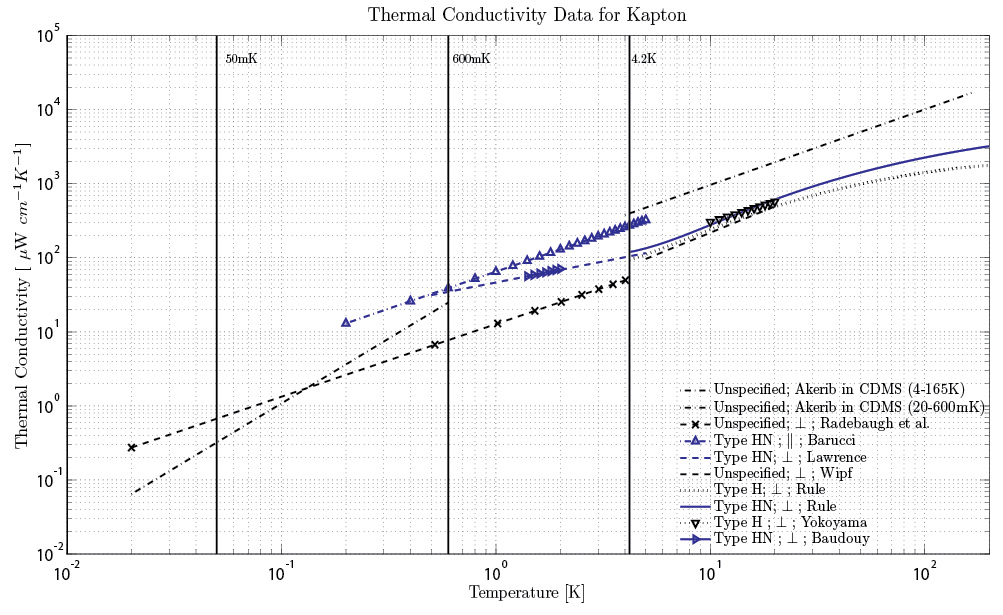
\includegraphics[width = .9\textwidth]{Kapton_var.png}
\caption{Compiled data for the thermal conductivity of Kapton films. The type is specified in the legend, as well as whether measurements were performed parallel or perpendicular to the Kapton surface. The direction of Kapton measurement is not stated when unknown. Data are from Radebaugh \cite{rad73}, Barucci \cite{bar}, Lawrence \cite{law}, Wipf \cite{wip}, Rule \cite{Rule1996}, Yokoyama \cite{yok}, Baudouy \cite{Baudouy2003}, and Akerib \cite{Akerib}. }
\end{figure}

\begin{table}[h]
\centering
\rowcolors{3}{gray!20}{white}
\begin{threeparttable}
\begin{tabular}{llclr}
\toprule
Author & Type & Dir. of Measurement & k(T) [ $\mu$W/cm-K] & Temperature Range [K]\\
\midrule
Wipf \cite{wip} & Unspecified & $\perp$ & $14.51 \cdot T^{1.177}$ & 5 - 20 \\
Lawrence \cite{law} & HN & $\perp$ & $46.38 \cdot T^{0.568}$ & 0.5 - 5 \\
Rule \cite{Rule1996} & HN & $\perp$ & $24.7 \cdot T^{1.043}$ & 4.2 - 10 \\
Rule \cite{Rule1996} & H & $\perp$ & $18.2 \cdot T^{1.121}$ & 4.2 - 10 \\
Barucci \cite{bar} & HN & $\parallel$ & $65 \cdot T$ & 0.2 - 5 \\
Radebaugh \cite{rad73} & Unspecified & $\perp$ & $12.73 \cdot T^{0.982}$ & 0.02 - 4 \\
Akerib \cite{Akerib} & Unspecified & ? & $60.7 \cdot T^{1.75}$ & 0.02 - 0.6  \\
Akerib \cite{Akerib}& Unspecified & ? & $92 \cdot T^{1.02}$ & 4 - 165 \\
Yokoyama \cite{yok} & H & $\perp$ & $36.87 \cdot 10^{0.9154}$ & 10 - 300 \\
Baudouy \cite{Baudouy2003} & HN & $\perp$ & $22.8 + 24.0 \cdot T$ & 1.4 - 2 \\
\bottomrule
\end{tabular}
\caption{Power law fits for thermal conductivity of Kapton in range of interest. The direction of measurement specifies whether thermal conductivity was taken parallel or transverse to the surface of a Kapton strip.}
\end{threeparttable}
\end{table}

\begin{figure}[h]
\centering
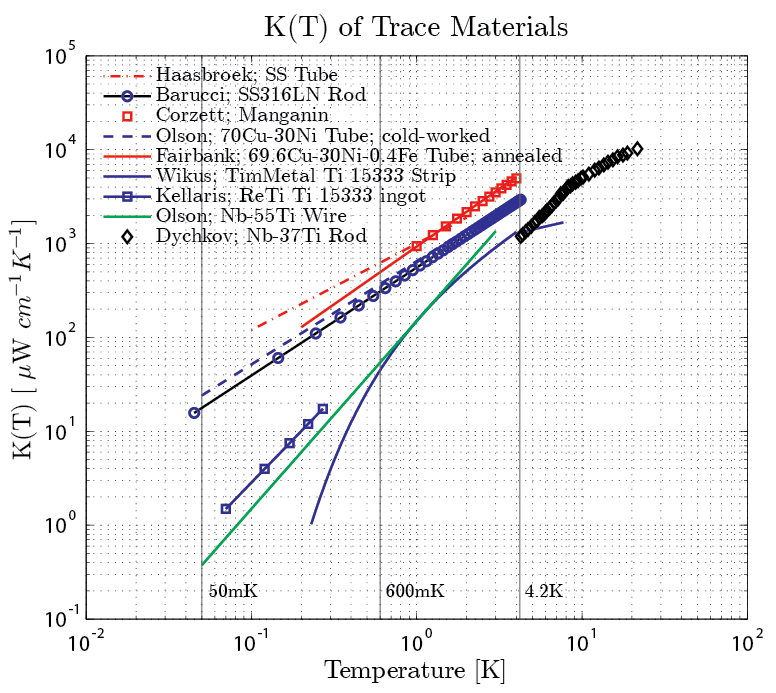
\includegraphics[width = .65\textwidth]{C:/Users/Niko/Documents/LaTex/Nick_K_Thesis/App_b_figs/trace_variation.png}
\caption{Thermal conductivities for trace materials. High and low values were taken from the literature when a significant variation was present among data. Notice that, based on thermal conductivity, TiMetal Ti 15-3-3-3 is the best candidate for all stages of the phonon cable. Data from: Barucci \cite{Barucci2008}, Corzett \cite{cor}, Olson \cite{ols}, Fairbank \cite{fair}, Wikus \cite{wik}, Dyachkov \cite{dya}, and Runyan \cite{run}.}
\end{figure}


\subsubsection{Thermal Conductivities of Trace Materials}

The thermal budget is very tight for the phonon line, as the thermal conductance is already expected to be much higher than for the current vacuum coax design, so thermal conductivity is a large consideration for trace material selection. Figure 5.2 presents the thermal conductivities of candidate materials; in the cases where differing thermal conductivities are given for a material, we give rough upper and lower limits on thermal conductivity (from a literature search and from our own testing).

From the figure, we see that Ti 15-3-3-3 has wildly varying thermal conductivities depending on the source and form of the material. The ReTi Ti 15-3-3-3 results were measured in our lab, and don't inspire confidence in Ti 15-3-3-3 sourced from companies besides TiMetal. We plan to verify the Wikus results for TiMetal Ti 15-3-3-3 in our lab soon to determine if the material truly exhibits such a steep drop in thermal conductivity for temperatures below its critical temperature of 3.9K \cite{wik}.

\subsubsection{Thermal Conductivity of Epoxy Adhesive}

The cable will likely be built using an epoxy adhesive to join layers together. The adhesive comes in a sheet which is then cured above room temperature. Unfortunately, we know next to nothing about the properties of the epoxy. This is worrisome, as epoxies (such as Stycast 1266) often have thermal conductivities above Kapton. Given that the majority of our cable will be epoxy (as described in section 4.3), we plan characterize the thermal conductivity of the epoxy as soon as possible.

\begin{figure}[h]
\begin{center}
\subfloat[]{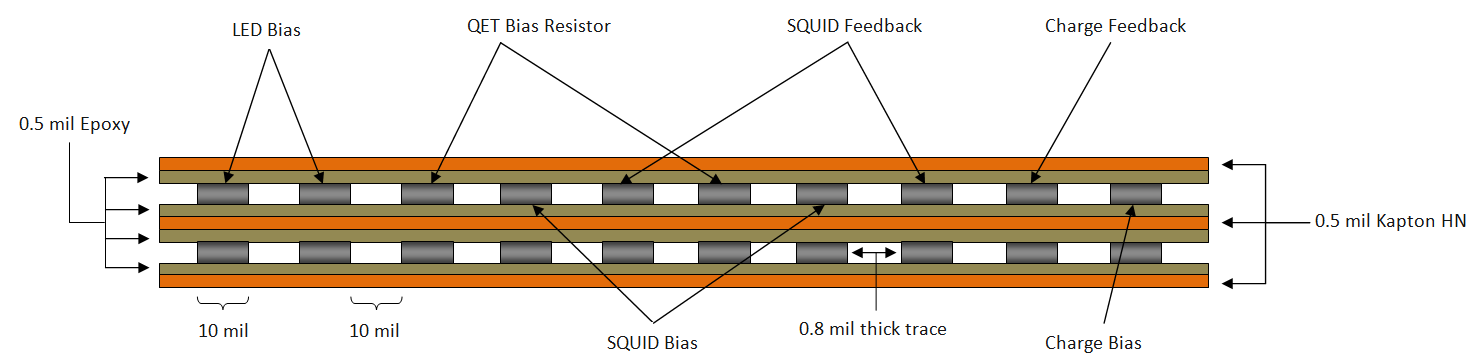
\includegraphics[width = .75\textwidth]{4K_600mK_diagram.png}}\newline
\subfloat[]{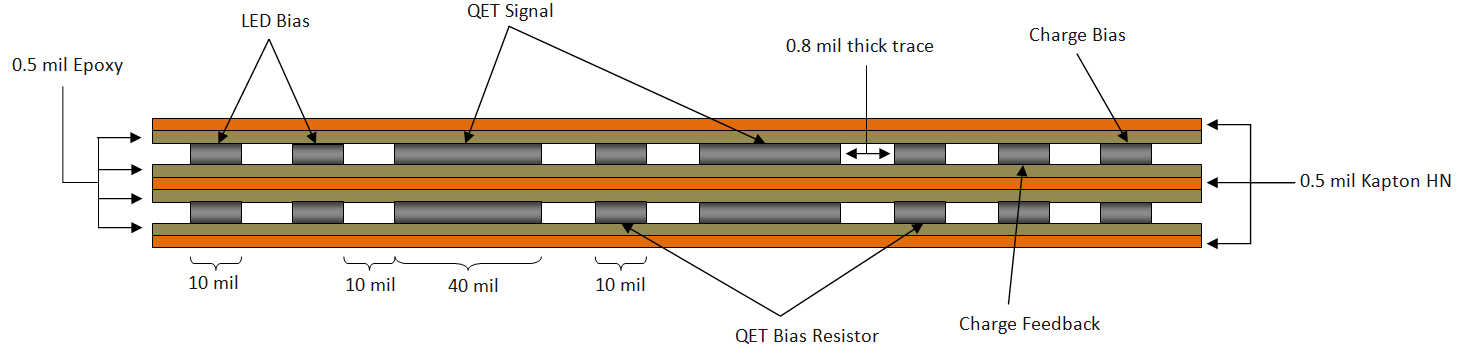
\includegraphics[width = .75\textwidth]{600mK_50mK_diagram.png}}\newline
\subfloat[]{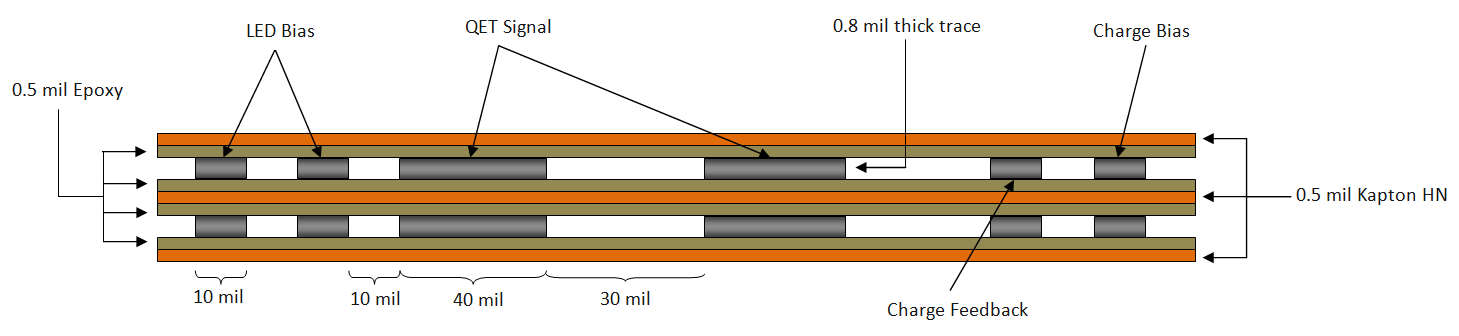
\includegraphics[width = .75\textwidth]{50mK_10mK_diagram.png}}
\caption{Representative cross-section for various stages of the parallel trace transmission line for phonon readout. (a),(b), and (c) show the cross sections for the 4K-600mK, 600mK-50mK, and 50mK-10mK spans respectively. All types of trace pairs are shown, but not all pairs of each trace type. The bottom traces in each figure are return lines.}
\end{center}
\end{figure}

\subsection{Phonon Transmission Line Layout and Dimensions}

Our collaboration has decided that a vertically-spaced parallel strip transmission line would best satisfy the required conditions for a phonon cable. A cross-section of the transmission line proposed is shown in Figure 5.3. It will be a multi-layer transmission line with individual signal/return lines vertically spaced, as shown in the figure. The design is similar to one used in EBEX cabling \cite{Polsgrove2009} for low inductance and low thermal conductance. The trace types are interleaved in order to decrease cross-talk between the SQUID signal lines. Throughout this section, keep in mind that our goal is to minimize cross-sections and material amounts, while satisfying other constraints.

The lists below give the full trace count for the proposed cable at different stages, as well as some useful dimensions for various calculations.

\begin{itemize}
\item 4.2K to 600mK
    \begin{itemize}
    \item 4.2K-600mK cable length = 9.24cm
    \item Trace width = 10 mil
    \item Total traces = $2\cdot12$ QET Bias Resistor + $2\cdot12$ SQUID Bias + $2\cdot12$ SQUID Feedback + $2\cdot6$ LED + $2\cdot4$ Charge Readout Bias + $2\cdot4$ Charge Feedback = 100 Traces
    \item Horizontal trace separation = 10 mil
    \item Trace thickness = 0.8 mil
    \item Total line width = 1.01 inches
    \item Total trace cross-section = 0.0052 $cm^2$
    \item Total Kapton cross-section = 0.0098 $cm^2$
    \item Total adhesive cross-section = 0.0130 $cm^2$
    \end{itemize}
\item 600mK to 50mK
    \begin{itemize}
    \item 600mK-50mK cable length = 5.04cm
    \item Trace width:
        \begin{itemize}
        \item QET Signal = 40 mil
        \item QET Bias Resistor, LED line, Thermometry line, Charge readout = 10 mil
        \end{itemize}
    \item Total traces = $2\cdot12$ QET Signal + $2\cdot12$ QET Bias Resistor + $2\cdot6$ LED + $2\cdot4$ Charge Readout Bias + $2\cdot4$ Charge Feedback = 76 Traces
    \item Horizontal trace separation = 10 mil
    \item Trace thickness = 0.8 mil
    \item Total line width = 1.13 inches
    \item Total trace cross-section = 0.0076 $cm^2$
    \item Total Kapton cross-section = 0.0109 $cm^2$
    \item Total adhesive cross-section = 0.0146 $cm^2$
    \end{itemize}
\end{itemize}

\begin{itemize}
\item 50mK to 10mK
    \begin{itemize}
    \item 50mK-10mK cable length = 3.25cm
    \item Trace width:
        \begin{itemize}
        \item QET Signal = 40 mil
        \item LED line, Thermometry line, Charge readout = 10 mil
        \end{itemize}
    \item Total traces = $2\cdot12$ QET Signal + $2\cdot6$ LED + $2\cdot4$ Charge Readout Bias + $2\cdot4$ Charge Feedback = 52 Traces
    \item Horizontal trace separation = 30 mil between QET ; 10 mil between all else
    \item Trace thickness = 0.8 mil
    \item Total line width = 1.13 inches
    \item Total trace cross-section = 0.0064 $cm^2$
    \item Total Kapton cross-section = 0.0109 $cm^2$
    \item Total adhesive cross-section = 0.0146 $cm^2$
    \end{itemize}
\end{itemize}

The motivation behind these dimensions, and the ones shown in Figure 5.3, comes primarily from cross-talk considerations, inductance requirements, and fabrication capabilities. The company which will likely fabricate our cable, Tech-Etch, uses photolithography to define the traces in a substrate. The trace widths and spacing of 0.01" are near the minimum they feel comfortable reliably producing. The Kapton and epoxy thicknesses are the minimum available through Tech-Etch, and the trace thickness was set based on the thinnest Ti 15-3-3-3 foil we were able to obtain. The trace thickness is flexible, however, depending on the materials we choose to use. To determine the SQUID signal trace widths we must now examine the expected inductance between signal/return trace pairs.

\subsubsection{Phonon Cable Inductance}

The phonon cable has inductance limits for the SQUID signal lines from the detectors to the SQUIDs due to frequency bandwidth considerations. The new SQUID design will reduce the superconducting QET resistance from 0.2$\Omega$ to 0.02$\Omega$. The 3dB roll-off frequency for our amplifier is proportional to the ratio R/L for the SQUID signal lines. Since the QET resistance will decrease by a factor of 10, the inductance must decrease as well to maintain a workable bandwidth.

We have set a limit of around 25nH between the SQUID signal/return lines. Assuming that the longest span we have between the SQUIDs and the detectors is 20", we have a mutual inductance limit of 25nH/20". To know if our cable will meet this limit, we used Sonnet EM modeling software to model the 50mK-10mK section of the cable (Figure 5.3c). We simulated two adjacent SQUID signal/return pairs with the dimensions given in the figure. The lines were modelled as lossless, as superconducting traces will be used in this section of cable. We also input the known properties of Kapton: relative permittivity = 3.4, dielectric loss tangent = 0.018, and dielectric conductivity (S/m) = 6.67E-16 from DuPont's website. We obtain an inductance of:
$$
L = 22.4\left[\frac{nH}{20"}\right]
$$
between signal/return lines. This number is below the maximum desired for our cable, so 40 mil wide traces satisfy our inductance requirements nicely.

As a sanity check for this number we can use an analytical formula which treats the traces as thin parallel plates:
\begin{eqnarray}
L \approx \frac{\mu_{0} \mu_{r} h}{w}
\end{eqnarray}

where L is the inductance per unit length of the trace pair, $\mu_{0}$ and $\mu_{r}$ are the magnetic constant and relative magnetic permeability respectively, h is the center-to-center vertical separation of the traces, and w is the width of the traces. For this formula to be accurate, we must have $w\gg h$ and $h > t$, where t is the thickness of the traces. With this formula we find
$$
L_{trace \ pair} = 31.9\left[\frac{nH}{20"}\right]
$$
which is larger than calculated from the Sonnet model. This likely represents the inadequacy of this simple model when the spacing of the traces is on the order of their thickness. However, the fact that they are not wildly different suggests that our model is performing correctly. To verify this, we ensured that our model limited to the analytical case for very large w, small t, and large h. The agreement between the Sonnet model and the analytical formula in this case was very good, inspiring confidence in the model.

\subsection{Resistivity of Trace Materials}
The phonon cable has two effective resistance requirements. The first is that the traces between the detectors and SQUIDs are superconducting. This is necessary to retain our phonon detection bandwidth ($dI/dP$, current change per power deposition) \cite{Pyle2012}. The second is a roughly defined maximum resistance of 100 ohms between the SQUIDs and room temperature for the phonon lines. This can be divided however we wish between the phonon cable (which goes to the 4K stage) and the 4K-300K cable. The resistivity of some candidate trace materials is shown in Table 5.2.

\begin{table}[h]
\centering
\begin{threeparttable}
\begin{tabular}{l|c|c|c|c}
Alloy & \multicolumn{3}{c}{Resistivity in $\mu$ $\Omega$ $cm$} \\\toprule
 & 300K & 273K & 10K & 4.2K \\\midrule
70Cu-30Ni & - & 38.4 & - & 36.4 \\
Constantan & 49.1 & - & 46.1 & - \\
Manganin (4\%Ni) & 47.6 & - & 41.9 & - \\
Ti15-3 & 146 & - & - & 173 \\
SS316 & - & 76.5 & - & 55.3 \\
50Nb-50Ti & 76.7 & - & 54 & 0 \\
BeCu & 8.3 & - & 5.6 & - \\
\end{tabular}
\end{threeparttable}
\caption{Resistivities of possible trace materials as a function of temperature. 70Cu-30Ni and SS316 data are from \cite{Clark1970}, Manganin, Constantan, and BeCu data are from Table 2.4 of \cite{Sciver1986}, NbTi data is from \cite{byc}, and Ti 15-3-3-3 data is from \cite{wik}. NbTi has zero resistivity at 4.2K because it is in a superconducting state. Notice as well that the temperature coefficient of Ti 15-3-3-3 is positive, unlike the other alloys.}
\end{table}

Originally, we had planned to have superconducting wiring for the full length of the tower. However, as stated above, we don't actually need zero resistance between the SQUIDs and the 4k stage. Instead, we just have to fall below a 100$\Omega$ limit for the wiring resistance above the SQUIDs (at 600mK). To explore a resistive trace option, we divide the candidates in Table 5.2 into two groups: superconductors and non-superconductors. Cupro-Nickel, Constantan, Manganin, and SS316 are not superconductors; they are resistive wiring. NbTi and Ti 15-3-3-3 are superconductors. However, the transition temperature of Ti 15-3-3-3 is 3.9K \cite{wik}; part of the cable would be in a superconducting state, and the other part in a normal state. We find in Appendix C that this will prevent Ti 15-3-3-3 from being used in the 600mK to 4K span of the phonon line. To see if the other resistive candidates would consume a reasonable portion of the resistance budget for the 600mK to 4K span, consider a trace of SS316 (the most resistive candidate material next to Ti 15-3-3-3) 0.01" (0.0254 cm) wide, and 0.00084" (2.134E-3 cm) thick. We find resistance from resistivity using
\begin{eqnarray}
R = \frac{\rho(T) L}{A}
\end{eqnarray}
where $\rho(T)$ is the material resistivity, L is the trace length, and A is the cross-section. We find
$$
\frac{R}{Length} = \frac{55 \cdot 10^{-6} \Omega cm}{5.42 \cdot 10^{-5} cm^{2}} = 1.014 \Omega / cm
$$

if we assume constant resistivity for SS316, given as the highest value for SS in Table 5.2. For the nominal length of the 4K-600mK stage given above (9.24cm), this yields 9.38$\Omega$. Though this is well below total resistance limit, this is a non-negligible portion of the 100$\Omega$. We will see in section 4.2 that we should be able to fabricate a 300K-4K line which falls below this remaining resistance budget, however, so a resistive trace could work for the 4K-600mK section. For 600mK-10mK, however, we are restricted to Ti 15-3-3-3, NbTi, or some other superconductor with $T_c$ well above 600mK. Now that we have both superconducting and non-superconducting options, we can examine the heat loads that each would result in.

\subsection{Phonon Transmission Line Heat Load}

The current design for a vertically spaced transmission line will conduct much more heat than a vacuum coax, and it is expected to contribute a significant amount to the overall heat load for the tower stages. Table 5.3 examines the expected heat loads for a phonon cable using different trace materials\footnotemark. The total heat loads were obtained by treating each portion of the cable separately (as if they were isolated) and summing the contributions. As you can see, the trace material contributes a significant amount to the cable heat load, especially on the Still (600mK/1K). This is where material choice becomes important. For 4.2K - 600mK, every candidate besides Ti 15-3-3-3 is a possibility. For 600mK and colder (SQUIDs to base temperature), the only options are superconducting traces, i.e. Ti 15-3-3-3 and NbTi. Though it is not listed in the table, the feasibility of Niobium as a trace option was explored and is discussed in Appendix D.

\begin{table}[h]
\resizebox{\textwidth}{!}{%
\begin{threeparttable}
\rowcolors{3}{gray!20}{white}
\begin{tabular}{rrrr|rrrr}
\toprule
 & \multicolumn{6}{c}{Heat Load for 48 Towers in $\mu$W} \\
  & 5K-1K & 1K-0.1K & 0.1K-40mK & 4.2K-0.6K & 0.6K-50mK & 50mK-10mK & Ref. \\
 \cmidrule(r){2-8}
   Ti 15-3-3-3 & 590-716 & 20-24 & 0.01-0.05 & 413-448 & 3.0-5.9 & 3\e{-3} - 8\e{-3} & \cite{wik},\cite{Run_ti153}   \\
   45Nb-Ti & 1047 & 23 & 0.03 & 624 & 5.0 & 3.7\e{-3} & \cite{ols}\\
   Manganin (2\%Ni) & 2476 & 193 & 1.3 & 1707 & 62 & 0.32 & \cite{Peroni1999} \\
   SS316 & 1347 & 118 & 0.9 & 941 & 39 & 0.24 & \cite{Barucci2008}\\
   70Cu-30Ni & 1483 - 2480 & 141 - 190 & 1.3 & 1047 - 1706 & 48 - 61 & 0.30 - 0.33 & \cite{pob},\cite{ols} \\
   Al5056 & 3.98\e5 & 2273 & 0.42 & 2.1\e5 & 321 & 0.03 & \cite{Coccia1983} \\
   Kapton & 238 & 20 & 0.27 & 171 & 7.3 & 0.08 & \cite{bar} \\
   Epoxy Adhesive $^{\dag}$ & 317 & 27 & 0.35 & 228 & 9.7 & 0.10 & \cite{bar}\\
   \multicolumn{2}{c}{\bf{Total Phonon Line}} & & & & & & - \\
   with Ti15-3 & 1145-1271 & 67-71 & 0.63-0.67 & 812-847 & 19.9-22.8 & 0.18 & - \\
   with 45Nb-Ti & 1605 & 70 & 0.65 & 1023 & 21.9 & 0.18& - \\
   with Manganin & 3031 & 240 & 1.9 & 2106 & 79 & 0.49 & -\\
   with SS316 & 1901 & 165 & 1.6 & 1340 & 56 & 0.41& -\\
   with 70Cu-30Ni & 2037-3034 & 188-237 & 1.9 & 1446-2105 & 65-78 & 0.48-0.51 & -\\
   with Al5056 & 3.99\e5 & 2319 & 1.04 & 2.05\e5 & 338 & 0.21 & - \\
   \multicolumn{3}{c}{\bf{Total Experiment Cooling Power}} & & & & &\\
 & 3000 & 2-50 & 1 & 3000 & 2-50 & 1 & \\
  \bottomrule
\end{tabular}
\end{threeparttable}}
\caption{Heat loads for constituents of the phonon cable as well as the total cable heat load for various materials for a total of 48 towers. Assumes all trace thicknesses are 0.84 mils, as this is the thickness of Ti 15-3-3-3 we have already procured for testing. The stage lengths assumed were 9.24cm (4.2K-0.6K), 5.04cm (0.6K-50mK), and 3.25cm (50mK-10mK). The powers given for each span are deposited on the lower of the two temperatures listed. The total predicted heat lift at the tower is given in the last row. All candidates are shown for all stages regardless of whether they can actually be used at that stage. This is simply for comparison purposes. \dag - Epoxy heat loads were calculated using Kapton thermal conductivity as a proxy.}
\end{table}

\footnotetext{Constantan (55Cu-45Ni) was proposed as an alternative to Cupro-Nickel (70Cu-30Ni), due to its lower Copper content. However, it was found to have a higher thermal conductivity than 70Cu-30Ni \cite{tou}. }

There are a few aspects of Table 5.3 which bear mentioning. The first is that the heat loads were calculated assuming that the 50mK stage is available for heat sinking. In the SuperCDMS Soudan towers, the 50mK stage is internal, so no wiring is heat sunk to it. The only external components of this stage on the tower face are two connectors for thermally linking the tower support tubes to the fridge Cold Plate. This works for the vacuum coaxes as they have a very small cross-section, thus a small thermal conductance. If we dont heatsink to the 50mK stage, we expect a heatload of over 20$\mu$W to the Mixing Chamber of the fridge (70$\mu$W assuming 1K-40mK stages) for a Ti 15-3-3-3 cable with the same dimensions presented in Table 5.3. The next aspect is that, depending on the temperatures, we are near or above the predicted heat lift capability at the tower (last column) for every stage. This makes design for the phonon cable crucial, as it will be a significant portion of the heat load; we will be pursuing options to decrease this heat load in the near future. One such option will be to bend the cable between stages, allowing it to snake its way along the tower between heatsinks. This would increase the effective length of the cable for thermal loading purposes; by equation 4.2, this would decrease the power load. Finally, since Aluminum is a common choice for trace material, we presented the heat loads for Aluminum 5056. This alloy was found to be similar to Aluminum 5052-H19 -- an alloy used by Tech-Etch -- so is used as a proxy to see if its expected heat loads would satisfy our requirements. The rationale behind choosing Aluminum is that development time would be significantly decreased through use of a well-understood material such as Aluminum. We find, however, that heat loads are far too high for such a material.

\subsection{Coefficients of Thermal Contraction}
Aspects of thermal contraction are important in the development of a laminated transmission line, as any differential contraction will cause internal stress in the cable. Stresses which are too high may cause the traces to delaminate from the Kapton substrate. This will have to be taken into consideration and tested for in the development phase.

\subsection{Conclusion}

Based on thermal conductivity and resistivity, NbTi is the clear choice for the entire length of the phonon line. It performs the second best thermally, and it is a superconductor for the entire temperature regime in which it would be used. Unfortunately, it is very difficult to obtain as a foil. For the time being, we have decided to use Stainless Steel 316LN\footnotemark for the 4.2K-600mK span,
\footnotetext{Grade 316LN refers to Low carbon content and Nitrogen-enhanced. This grade has lower radioactivity levels than 316, very low magnetic permeability, and higher yield strength than 316 without loss of ductility.}
and Ti 15-3-3-3 for the 600mK-50mK span and 50mK-10mK span.\footnotemark

\footnotetext{As stated in 4.1.3, Ti 15-3-3-3 becomes brittle at low temperatures. The effect of this on a phonon cable design is considered in Appendix E.}

\section{Charge Readout Lines}

The form of the future charge readout lines is still under debate. Since noise is only a concern on the gate wires, the charge feedback and bias pairs can be integrated into the flexible parallel-trace transmission line design. The 4 remaining gate wires have a few available options. The simplest option would be for the lines to remain vacuum coaxes. The next option involves a flexible coaxial cable produced by AXON'. The last option would be to make our own cable with low noise properties.

\begin{figure}[ht]
\centering
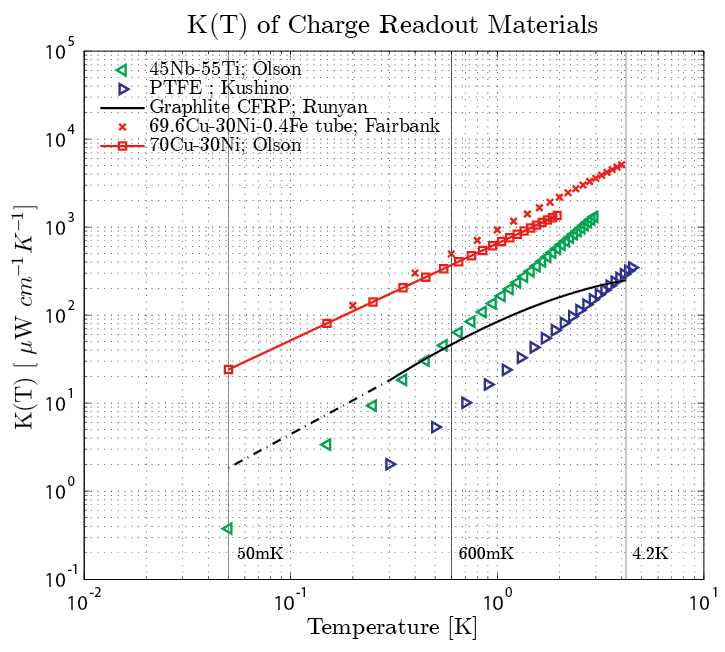
\includegraphics[width = .6\textwidth]{C:/Users/Niko/Documents/LaTex/Nick_K_Thesis/CH4_figs/Charge_matl_K.png}
\caption{Thermal conductivities of materials used to model heat conduction in the charge readout designs. CuNi and PTFE are used as proxies for Constantan and Celloflon (porous PTFE) respectively. Data are from Runyan \cite{run}, Olson \cite{ols}, Fairbank \cite{fair}, and Kushino \cite{kus:cu}. The dashed line is a fixed exponent extrapolation of Graphlite data used in thermal conductance calculations.}
\end{figure}

If we keep the vacuum coaxes, we will alter the design slightly to allow removal of the coaxes from the tower. This would involve a type of carbon fiber rod supported frame to which the wires are mounted, as depicted in Figure 5.4. Though this could be a low heat load design, it is the least convenient option, as it requires the use of the same copper side coaxes used in SuperCDMS Soudan towers. Heat loads for this option are presented in Table 5.4. The wires would be the same 0.0012" diameter Nb-47\%Ti lines currently used in our towers -- provided by Tekdata -- however they would have an additional heat sink at the newly available externalized 50mK stage on the next generation tower design.

The next option involves a coaxial cable from AXON' \footnotemark.\footnotetext{Another company, Texcal, was considered, as they also produce low-noise cabling. Unfortunately, their cables use silver-plated copper conductors, whose thermal conductivity far exceeds what is acceptable for our purposes.}
This cable uses Constantan as a conductor material, PTFE for a housing, and Celloflon dielectric (porous PTFE); The cable's cross-section is shown in Figure 5.4 on the left. A thin graphite coating on the outside of the Celloflon dielectric prevents static charge build-up on the insulator -- our main source of noise in the gate wires. The suitability of this option depends on expected heat loads from the cable. These are shown in Table 5.4. The calculations use Cupro-Nickel (70Cu-30Ni) thermal conductivity in place of Constantan \footnotemark, as well as simple PTFE in place of Celloflan.

\footnotetext{It was found that the actual thermal conductivity of Constantan is slightly higher than Cupro-Nickel, but is close enough for approximation purposes. If this is considered a viable option, more accurate calculations will be done.}

Another option is to simply alter a cable to have low-noise characteristics. This could be made possible with a flexible polyimide cable whose dielectric has undergone ion implantation to increase the conductivity to near that of graphite \footnotemark. This would serve the same function as the graphite layer in the AXON' coaxial cable -- preventing static charge build-up. Heat loads for this option are not presented, as the potential form of these cables is as-of-yet unknown.

\footnotetext{See, for instance, \cite{Chen2009}}

\begin{figure}[h]
\centering
$\vcenter{\hbox{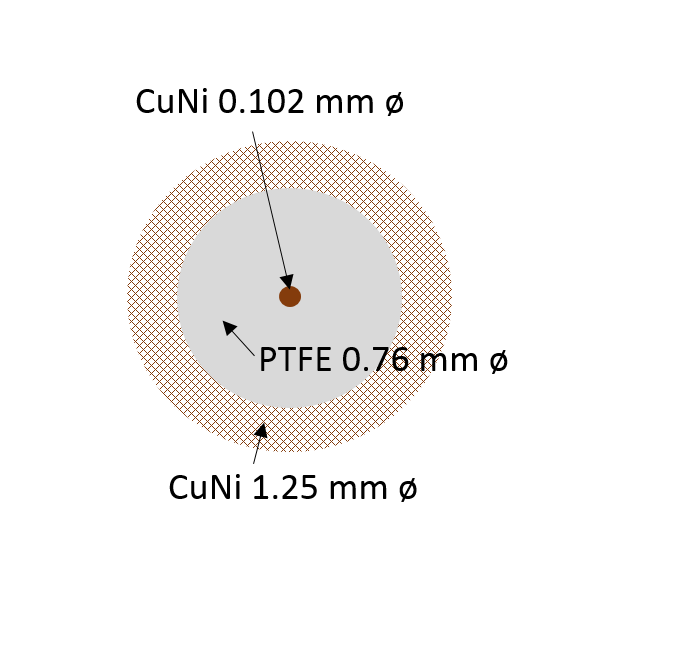
\includegraphics[width = .2\textwidth]{C:/Users/Niko/Documents/LaTex/Nick_K_Thesis/CH4_figs/Axon_cable_model.png}}}$
$\vcenter{\hbox{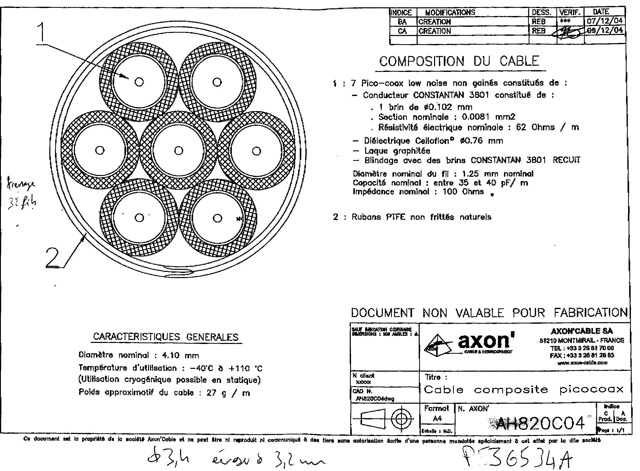
\includegraphics[width = .5\textwidth]{C:/Users/Niko/Documents/LaTex/Nick_K_Thesis/CH4_figs/Edelweiss_cable.jpeg}}}$
$\vcenter{\hbox{\includegraphics[width = .45\textwidth]{C:/Users/Niko/Documents/LaTex/Nick_K_Thesis/CH4_figs/Vacuum_coax_model.png}}}$
\caption{Two possible designs for future charge gate wires. Top is the specially made AXON' cable (manufactured to have a Constantan conductor). Each bundle of the cable contains 7 coaxes (marked by a 1 in the diagram). The upper left is the model used for thermal conductance purposes. Bottom shows the basic structure of a removable vacuum coax design with copper heatsink connections supported by carbon fiber rods.}
\end{figure}

\subsection{Charge Readout Heat Loads}

To get expected heat loads for the charge readout options, we examine two
The total charge readout wiring heat load contribution for a 48 tower experiment is presented below in Table 5.4. These calculations assume 4 gate wires per detector, so 24 wires per tower, and 1152 wires for 48 towers (or 1152 coaxes in the case of the AXON' cable).

The models used for thermal conductance calculations are shown in Figure 5.4; the relevant thermal conductivities are shown in Figure 5.5. The vacuum coax assumed two 0.04" Graphlite CFRP rods supporting four 0.0012" NbTi wires between each stage (per detector). The AXON' cable model is a simplification of the actual design, and is shown in the upper left of Figure 5.4. We use the thermal conductivity for CuNi as a proxy for Constantan, and model the center conductor and shielding as solid cross-sections. The Celloflon is modelled as solid PTFE. To find total heat loads for the charge readout options, we add the contributions of each element separately.


\begin{table}[h]
\resizebox{\textwidth}{!}{%
\rowcolors{3}{gray!20}{white}
\begin{threeparttable}
\begin{tabular}{rrrr|rrr}
\toprule
 & \multicolumn{6}{c}{Charge Coax Heat Loads for 48 Towers in $\mu$W} \\
  & 5K-1K & 1K-100mK & 100mK-40mK & 4.2K-600mK & 600mK-50mK & 50mK-10mK \\
 \cmidrule(r){2-7}
 \multicolumn{2}{c}{\bf{Vacuum Coaxial Cable}} & & & & \\
   Graphlite Rods & 731 & 35 & 0.16 & 566 & 11 & 0.036 \\
   NbTi Wires & 10.3 & 0.08 & 7.7\e{-5} & 6.1 & 0.018 & 1.0\e{-5} \\
   Total Vacuum Coax & 742 & 35 & 0.16 & 572 & 11 & 0.036 \\
   \multicolumn{2}{c}{\bf{AXON' Coaxial Cable}} & & & & \\
   Center Conductor & 81 & 2.8 & 0.019 & 57 & 0.98 & 5.1\e{-3} \\
   Celloflon Dielectric & 365 & 3.5 & 4.1\e{-3} & 222 & 0.79 & 5.8\e{-4} \\
   Constantan Shielding & 7701 & 269 & 1.8 & 5435 & 92 & 0.49 \\
   Total AXON' Cable & 8147 & 276 & 1.87 & 5714 & 94 & 0.49 \\
    \multicolumn{3}{c}{\bf{Total Experiment Cooling Power}} & & & & \\
 & 3000 & 2-50 & 1 & 3000 & 2-50 & 1 \\
  \bottomrule
\end{tabular}
\end{threeparttable}}
\caption{Heat loads for charge readout coaxes for 48 towers with removable vacuum coax option and AXON' cable option in terms of constituent materials and total heat loads. The last row gives current estimated heat lift capability at the tower. Vacuum coax numbers assume cable lengths of 5.08cm (2") for every stage. AXON' cable numbers assume twice this length (10.16cm) given their ability to flex. Assumes 4 lines (or coaxes) per detector, 6 detectors per tower. The vacuum coax calculations assume two 40 mil diameter rods between each stage, which constitute the frame for the removable vacuum coaxes. The AXON' cable uses CuNi data from \cite{ols} as a proxy for Constantan, and solid PTFE conductivity from \cite{kus:cu} as a proxy for Celloflon (a porous PTFE). We see that the Graphlite rods and Constantan shielding dominate the heat loads.}
\end{table}

\subsubsection{Remarks}
We see that the heat loads for the vacuum coax option are rather large, due to the carbon fiber rods. While the calculations have assumed a 0.04" rod thickness, our supplier \footnotemark for rods also has 0.033", 0.03", 0.02", and 0.01" diameter rod options, which would reduce heat loads. In contrast, the expected heat loads from the AXON' cable certainly rule it out as a candidate for replacing the vacuum coax design. Though the thermal conductivities used in the model for the AXON' cable were not the actual materials, we expect that heat loads are similar. Using solid PTFE instead of porous Celloflon gives a higher thermal conductivity, but since the shielding dominates, this will have little effect. In addition, the CuNi thermal conductivity used in calculations was the lower limit in the data, so we expect heat loads to be higher in reality.

Until a better solution is found, we have decided that the best option for the charge read-out is a removable vacuum coax supported for Graphlite rods.


\footnotetext{Diversified Structural Composites. 1512 Interstate Drive, Erlanger, KY 41018 USA.}

\section{300K - 4K SNOLab Cable}

The last major wiring component which this work will discuss is the 300K-4K SNOLab cable, which will run from room temperature (300K) to the warmest tower stage (4.2K). The design for this cable is still in its infancy, but we have two rough specifications to design to: First, we will have two trace types: "high resistance" traces which are allowed a resistance of up to 100$\Omega$ from 300K-4K, and "low resistance traces, whose resistance will be between $\sim$5-10$\Omega$\footnotemark . Second, we must ensure that we fall below the heat lift capability of the fridge -- estimated to be roughly 1.35W for the 48-tower experiment. Apart from these considerations, the cable must be thin enough to be flexible, the dimensions must be work-able (not too wide, robust, etc.), and the traces should be solderable. This section discusses expected resistances and heat loads for a few trace material options.

\footnotetext{These limits will be lower if we use a resistive trace for the phonon cable.}

\subsubsection{Cable Layout}

The 300K - 4K cable will start at room temperature and travel through the fridge, terminating at the 4.2K stage of the tower. Figure 5.6(a) shows a mock-up of a possible cable design which will be used to calculate heat loads onto the fridge. The total available length for the cable -- based on fridge set-up -- is around 130". The cable will run 20" from 300K to a 50K heatsink. From here, we allow 85" between the 50K heatsink and the 4.2K heatsink. The last 20" of the cable goes from the 4.2K heatsink to the 4.2K stage of the tower.

The trace layout of the cable will allow for low resistance and high resistance traces. This differentiation allows for small cross-sections (higher resistances) where resistance isn't as important, in order to minimize heat loads to the fridge. There will be 106 high resistance traces, with up to 100$\Omega$ per trace. There are only 10 low resistance traces ($\sim 5 \Omega$) which are ground returns. The dimensions of these lines will be set by these resistances and trace material resistivity.

We see in Figure 5.6(b) a representative cross-section of a possible cable design, which uses a vertically-spaced transmission line layout. The trace layers will be surrounded by Kapton layers which are attached with an epoxy adhesive. Assuming a company such as Tech-Etch fabricates this cable (as with our phonon cable) we have an epoxy thickness of 0.0005" and a Kapton thickness of $\geq$0.0005" (depending on the desired robustness of the cable). The widths of the low and high resistance traces will be set through resistance requirements. The trace thicknesses will be set independently for each material.

\begin{figure}[ht]
\centering
\subfloat[]{\includegraphics[width = .5\textwidth]{C:/Users/Niko/Documents/LaTex/Nick_K_Thesis/CH4_figs/300K_cable_diagram.png}}
\subfloat[]{\includegraphics[width = .6\textwidth]{C:/Users/Niko/Documents/LaTex/Nick_K_Thesis/CH4_figs/300K_cable_cross_section.png}}
\caption{300K-4K model for resistance and heat load estimates. (a) shows length and heat sink locations. Each heat sink is assumed to be wide enough for perfect heatsinking. (b) shows a representative cross-section of the cable with 8 of the 116 total traces. 10 traces will be low resistance ground return lines, while the rest may be high resistance. X and Y are the width of the high resistance and low resistance traces respectively, and will be determined for each material. This cross-section assumes that the ground returns can be vertically spaced.}
\end{figure}


\subsection{Thermal Conductivity and Electrical Resistivity of Trace Materials}

We expect that the cooling capacity of our fridge at the 4.2K stage will be such that heat loads will not be the primary concern for the 300K-4K cable. Instead, the primary factors which set cable dimensions and determine material viability are the resistance limits given previously. To this end, we must consider the resistivities of all trace materials, given in Table 5.2. These are used to calculate minimum cross-sections for the two trace types by rearranging equation 5.2. The minimum cross-sections for high resistance traces (type X) and low resistance traces (Y) are given in Table 5.5. In calculating minimum cross-section, all resistivities were assumed constant over the temperature range, with the highest value selected to be conservative. Be-Cu is the only exception. Its temperature-dependent resistivity is given in \cite{Sciver1986}. The results of the calculations are discussed in the next section.
To ensure our secondary requirement of manageable heat loads, we present the thermal conductivities of each material in  Figure 5.7. We provide the thermal conductivity of Kapton for comparison, as any transmission line-type cable would use Kapton as a substrate. We can see the wide range of trace material thermal conductivities (which are, not surprisingly, roughly inversely proportional to each of their resistivities). In addition, the very low thermal conductivity of Kapton leads us to expect heat loads which are dominated by trace selection.

\begin{figure}[ht]
\centering
\includegraphics[width = .7\textwidth]{C:/Users/Niko/Documents/LaTex/Nick_K_Thesis/CH4_figs/300K_trace_and_kap_Kt.png}
\caption{Thermal conductivities of trace candidates for the 4.2K to 300K cable. Kapton is included for comparison, as it will be used as a substrate material in the cable. References for data are: Nb47Ti - \cite{Blake} ; Nb50Ti - \cite{Flachbart1978} ; Ti 15333 - \cite{Canavan2006} ; Manganin (84Cu-4Ni-12Mn) - \cite{tou} ; 70Cu-30Ni - \cite{Blake} ; 55Cu-45Ni - \cite{tou} ; SS316 - \cite{ss316_nist} ; Kapton - \cite{Rule1996}.}
\end{figure}

\subsection{Trace Material Performance}

Table 5.5 gives an overview of important performance aspects of some trace materials: Cable width, Trace dimensions, and Expected heat loads. Minimum trace dimensions are calculated assuming constant resistivities for all resistive materials except Be-Cu (Copper excluded). Trace heat load contributions\footnotemark for all 48 towers are calculated assuming the presence of a 50K heatsink along the cable, and lengths given in Figure 5.6.  Below we examine some aspects of this table for each trace material.

\footnotetext{Even with outer layer thicknesses of 3 mil the contribution to total heat load from Kapton is below 10\% for even the least conductive trace material; it was excluded for simplicity.}

\begin{table}[h]
\resizebox{\textwidth}{!}{%
\rowcolors{3}{gray!20}{white}
\begin{threeparttable}
\begin{tabular}{l|ccccccc}
\toprule
Material & \multicolumn{2}{c}{$A_{min}$ [$in^2$]} & Thickness [in] & \multicolumn{2}{c}{Width [in]} & Cable width [in] & Power to 4.2K [mW] \\
& X & Y & & X & Y & & \\
\midrule
OFHC-Cu(rrr=100) & - & - & 0.0002 & 0.005 & 0.005 & 0.619 & 810 \\
Manganin (4\%wt Ni) & 2.5\e{-5} & 5.0\e{-4} & 0.003 & 0.0084 & 0.1675 & 1.87 & 133 \\
70Cu-30Ni & 2.0\e{-5} & 3.9\e{-4} & 0.003 & 0.0065 & 0.131 & 1.59 & 172 \\
Be-Cu & 3.5\e{-6} & 7.0\e{-5} & 0.001 & 0.007 & 0.070 & 1.31 & 82 \\
Ti 15-3-3-3 & 8.9\e{-5} & 1.8\e{-3} & 0.004 & 0.022 & 0.443 & 3.97 & 69 \\
SS-316 & 3.9\e{-5} & 7.9\e{-4} & 0.004 & 0.0098 & 0.196 & 2.09 & 144 \\
\midrule
 \multicolumn{4}{l}{\textbf{Total Experimental Cooling Power @ 4.2K}} & & & &  1350 \\
\bottomrule
\end{tabular}
\end{threeparttable}}
\caption{Comparison of trace material performance for the 300K-4K cable, assuming a two trace layer transmission line design. X \& Y refer to the dimensions of the high resistance (100$\Omega$ lines and the low resistance ($\sim 5\Omega$) lines respectively. $A_{min}$ is the minimum cross-section allowable to fall at or below these resistances for each material. These were calculated assuming the highest resistivity number in Table 5.2 for each material, with the exception of Be-Cu, whose temperature dependent resistivity was used, from \cite{Sciver1986}. The trace thickness is assumed for each separately to provide as reasonable trace widths as possible. An approximate cable width is given for a single cable of 116 traces. The last column gives the  heat load on the 4.2K stage of the fridge for 48 towers (6 cables per tower), only counting trace contribution (which is over 90\% of the total cable heat load). The last row gives the total experimental cooling power for the dilution fridge. Copper and Ti 15-3-3-3 are included to give an idea of extremes, i.e. high thermal conductivity -- low electrical resistivity and low thermal conductivity -- high electrical resistivity. X \& Y widths and trace thickness for Copper, and X widths for Be-Cu were limited by production capabilities of Tech-Etch, rather than resistance limits.}
\end{table}

\textbf{OFHC Copper:} Copper is mainstay of cryogenic electronics, so naturally it was considered here. It is easily soldered, and has a low $\rho$. In fact, its dimensions are limited by fabrication capabilities rather than resistance limits. Despite this, the expected heat loads are very high for the experiment -- $\sim$5 times higher than the next closest option. In addition, the only way to get the small dimensions given in Table 5.5, it would need to be sputtered. This renders it fragile.

\textbf{Manganin:} Manganin is a resistive metal, whose thermal conductivity is fairly low. It is also solderable. Its high resistivity would require fairly large dimensions to accommodate our resistance requirements, however.

\textbf{70Cu-30Ni:} Cupro-Nickel performs slightly better than Manganin. It has a slightly lower $\rho$, but higher thermal conductivity. It is solderable, and gives reasonable expected heat loads as well.

\textbf{Be-Cu:} Beryllium Copper is the least resistive candidate material besides OFHC Copper. The width for the high resistance trace is actually set by the capabilities of Tech-Etch rather than resistance. It was given a thickness of 0.001" to ensure strength. We see that the heat loads and cable widths expected from Be-Cu are very reasonable. It is also very easy to solder.

\textbf{Ti 15-3-3-3:} Ti 15-3-3-3 was included to show how a very resistive, low thermal conductivity material performed. We see that despite its very low thermal conductivity it only slightly outperforms Be-Cu; however, the cable widths and trace thicknesses required are unworkable. In addition, it is incredibly difficult to solder to other materials.

\textbf{SS-316:} Stainless steel is a candidate similar to Ti 15-3-3-3. It is on the lower end of the thermal conductivity spectrum, and the upper end of the electrical resistivity spectrum. Though heat loads are reasonable, we see that dimensions required for a SS trace to work are likely too large for our experiment (a 4 mil thick trace would not be flexible). Considering the difficulty in soldering to SS, it is not a desirable option.

Considering that the main requirements of the cable are resistance limits, workable dimensions, and solderability, it is clear that of these materials, Be-Cu is the ideal option. As the design and requirements of this cable are still in development, this may change. This section is simply meant to provide a first-pass examination of material options and cable lay-out.

\chapter{Conclusions and Further Investigation}

\section{The Case for Dark Matter}
The dark matter problem is an interesting one; though we have zero direct evidence for dark matter, we have a plethora of indirect evidence. Chapter 1 briefly outlined the argument for dark matter and its potential properties in a $\Lambda$CDM Model of cosmology. This included observational evidence such as velocity dispersion in galaxies, rotation curves of spiral galaxies, and gravitational lensing effects which suggest a large amount of non-luminous matter on large and small scales. We saw that this dark matter would likely be non-baryonic in nature due to big bang nucleosynthesis element ratios in the modern universe. This is further evidenced by baryon acoustic oscillations in the universe and the CMB, which suggest huge potential wells of non-interacting dark matter as seeds for structure formation.

\subsubsection{WIMP dark matter}
We found that WIMPs satisfy the requirements for a dark matter candidate very well; they produce an expected relic density on par with what is expected for non-baryonic dark matter, and the existence of a new particle near their expected energy (100GeV) is predicted by the standard model.

\subsubsection{Direct detection}
Direct detection is the ultimate goal for dark matter theory, as it would allow us to characterize the new particle with little doubt. Many experiments throughout the world are using a variety of techniques in an effort to directly detect dark matter. CDMS is just one such experiment; however, it is one of the leading experiments in the world, setting some of the most stringent parameter spaces through the use of Ge and Si detectors which collect both ionization and phonon signals from events in the detectors to give our experiment the best background rejection of any experiment.

CDMS data has already detected three possible light WIMP events which merit further exploration. The next generation of CDMS -- SuperCDMS SNOLab -- plans to further improve the experiment with iZIP (interleaved phonon and ionization sensor) detectors, increased 1kg detector mass, and significantly more overall detector mass, aiming for 200kg in the final phases. In addition, it will be located in a mine in Sudbury in Ontario, Canada which promises cosmogenic backgrounds which are reduced by a factor of $\sim$1000. With the development of SuperCDMS SNOLab and numerous other experiments throughout the world (XENON, CRESST, EDELWEISS, etc.) the possibility of dark matter direct detection in the near future looks promising.

Though SuperCDMS SNOLab holds promise for the future, it must first be designed. Increasing our detector mass from 10kg to 200kg, and increasing signal readout will require significant improvements in design. This work has attempted to outline some of the technical considerations which which must go into the SuperCDMS SNOLab tower. To that end, I have described some of the main components of this tower -- thermal stand-offs, phonon readout lines, charge readout lines, and the 300K-4K cable -- the current constraints to their design, and possible solutions to help CDMS move forward with the design of the next generation experiment.

\section{Thermal Conductivity Measurements}

Since many of the constraints on tower design will be thermal in nature, we must be sure to characterize the thermal conductivity of all our candidate materials. For this purpose we have carried out a series of thermal conductivity tests in our 75$\mu$W dilution refrigerator. Through these tests, we found a few interesting candidates for the tower thermal stand-offs. Vespel SCP-5050 was found to have even lower thermal thermal conductivity than Vespel SP-22, and Vespel SCP-5000 had a similar thermal conductivity to SP-1. We found that ReTi Ti 15-3-3-3 didn't follow the same interesting behavior as TiMetal Ti 15-3-3-3, though it had similar thermal conductivity above 1K, so it isn't a desired material. Graphlite CFRP's thermal conductivity was verified to be low enough to make it a likely candidate given its impressive strength.

The three methods used to measure thermal conductivity -- standard method, parameter-fit method, and the differential method -- were all found to be valid, useful methods, each with their own set of strengths. The standard method is particularly useful when one cannot ensure a strong thermal link to a cooling reservoir and has two well-calibrated thermometers. The parameter-fit method was found to be useful when we had a clear equation form to fit to for thermal conductivity. It would also be useful if the thermal conductivity was found to be strongly dependent on temperature. The differential method is most useful if a strong thermal link to a cooling reservoir is possible. If so, it offers very accurate results by eliminating constant parasitic heat loads and calibration differences between thermometers.

We are planning numerous future tests: Graphite grade 2020, TiMetal Ti 15-3-3-3, Kapton/epoxy sheets, TiMetal Ti21s. These tests will explore more tower stand-off options, and -- more importantly -- characterize the thermal conductivity of key components in the tower electronic connections. The design of our tower may have to be adjusted depending on the results of these future tests (e.g. if we find that the Kapton/epoxy composite has high thermal conductivity, the phonon line design may need alteration).

\section{Tower Thermal Stand-offs}

The thermal stand-offs are meant to support our experiment "tower" which houses detector electronics, supports the electronic connections, provides heat-sinking, and supports the detectors. They thermally isolate the various temperature stages of the fridge while physically connecting them. The thermal stand-offs will be designed to meet thermal, radioactivity, mechanical, and stability requirements in our tower.

First we examined thermal, radiogenic, and strength properties in each material. We found that many materials had a lower thermal conductivity than UF-4S graphite (currently in use as a stand-off). Graphlite and Ti 15-3-3-3 had a higher thermal conductivity, but their strength easily compensates. Next, to ensure low background in our experiment, we screened each of our samples for radioactivity. We found that Graphlite, Ti 15-3-3-3, Vespel SCP-5050, Vespel SP-1, and POCO graphites had reasonable levels of radioactivity (below 20mBq/kg for Th-232, U-238, K-40, Co-60, Cs-137). Vespel SCP-5050, surprisingly, had much lower radioacivity levels than SP-22. We also found that POCO graphites were very effectively purified in a process offered by both POCO and Mersen; a high-pressure heated chlorine gas is used to remove heavy metal impurities from the bulk of the material. AXM-5Q activity was reduced between a factor of 50-100. We then used a program called Sources4C to model neutron emission from our tower stand-offs, as this is the most difficult background to veto. The numbers obtained are still preliminary, but we expect reasonable neutron emission levels From here, we considered some thermo-mechanical properties of each material. We found that Graphlite, Ti 15-3-3-3, and Ti 12s offer the highest strength. Vespel SCP-5050 and SCP-5000 were found to be significantly stronger than their SP counterparts, giving them favor as candidate materials. All materials considered were significantly stronger than UF-4S graphite. We considered the thermal stability of each material and found that the thermal contraction of every material besides Vespel SP-1 was low enough to prevent failure of the charge lines.

Once we characterized the materials, we considered two structures for use as thermal stand-offs: hexapods and tubes. An analytical model was developed for analysis of the tubes. This model developed a theoretical method to replicate the DPA performed on the Soudan tower tubes (transverse load) and considered four failure modes: Bending buckling, shear buckling, normal material failure, and shear material failure. This model reproduced the graphite DPA with discrepancies of $\sim$20\%, which could likely be explained by the fact that we do not know the mechanical properties of UF-4S well. From here, we found optimized dimensions from this model for each candidate material which should minimize both radioactivity and heat loads from the stand-offs. Resulting heat loads indicate that multiple materials -- primarily Graphlite CFRP, TiMetal Ti 15-3-3-3, and Vespel SCP-5050 -- can satisfy our tower thermal stand-off requirements. They allow heat loads to each stage which are reduced by up to a factor of twenty from the previous material (UF-4S graphite) and its current dimensions. We are in the process of developing FEA models which will aid in characterizing the tube and hexapod structures. We are also developing test structures which will allow us to mechanically load prototype tower stand-offs and test properties such as shear strength, compressive strength, and tensile strength.

\section{Wiring for the Tower}

The next major development in the tower that we considered was the tower wiring. This wiring is broken up into three main components: 300K-4K cabling, phonon readout, and charge readout. This wiring had numerous constraints imposed by the experiment requirements; this work examined thermal, resistance, inductance, and practical constraints.

\subsubsection{Phonon Cable}
First we explored the possibility of a vertically-spaced parallel trace transmission line for the phonon cable from 4.2K-10mK on the tower, to replace the mounted vacuum coaxes currently used. We will likely have this fabricated by a company called Tech-Etch. We examined the thermal conductivities of transmission line components; this included Kapton as a substrate material, and numerous trace materials. We found that two titanium alloys, NbTi and Ti 15-3-3-3 offer the best thermal conductivities over the range 10mK-4K.

For this cable, inductance requirements limit us to $\sim$25nH over the length of the phonon cable from the SQUIDs at 600mK to the detectors. Using EM modeling software, Sonnet, we calculated the expected inductance for these vertically-spaced trace pairs. We found that we are able to satisfy this requirement with traces 40 mil wide, giving a reasonable width cable overall ($\sim$ 1").

Next we considered the resistance requirements for the phonon line. The first requirement calls for superconducting traces from the detectors to the SQUIDs (at the Still); the second requires either superconducting traces or low resistance traces from the SQUIDs to the 4.2K stage. The candidate materials characterized were NbTi (superconducting, $T_c \sim 10K$), Ti 15-3-3-3 (superconducting, $T_c \sim 4K$), SS316LN, Cupro-Nickel, and Manganin. We saw that the phonon line will be difficult to design thermally, due to the large increase in material in moving from a vacuum coax to a transmission line. We found that the ideal trace material would be NbTi, which is superconducting along the entire length of the phonon cable. Due to difficulty in obtaining NbTi as a foil, we have decided for now to use SS316LN traces from 4K to the Still, and superconducting Ti 15-3-3-3 traces from the Still to base. The outstanding problem for the phonon cable currently is thermal in nature. We are quickly approaching the cooling power of the total experiment with just the phonon cable contribution. This must be addressed soon to ensure a successful experiment.

\subsubsection{Charge Lines}
The next wiring component we considered was the charge readout lines, which must have very low noise between the detectors and their amplification at the HEMTs at 4K. These cannot be integrated into the phonon line because the primary source of noise for them is static charge build-up on dielectric components of the cabling. We considered cables by two companies, AXON' and Texcal, who use a semiconductive layer on the dielectric (such a graphite) to prevent static charge build-up, but found heat loads to be far too high for our experiment. For the time being, we have decided to remain with a vacuum coax design that is removable from the tower. These vacuum coaxes would still be made out of NbTi wires, and would remain under tension through the use of permanently attached struts which provide a rigid frame after removal from the tower face. We found that thin graphlite rods $\leq$0.04" diameter would serve this purpose well without introducing large heat loads. These struts would, however, greatly dominate the overall heat load from the charge readout design; therefore, we are continuing to search for another more ideal solution.

\subsubsection{300K-4K Cable}
Finally, we briefly discussed a potential design for the 300K-4K cabling which plugs in to the 4K stage of the tower. This design would be a transmission line very similar in design to the phonon cable, roughly 130" long, with a 50K heatsink and a 4K heatsink between room temperature and the tower. The current constraints on this cable are tentative but have been outlined in this work. First we have the resistance limit of 100 $\Omega$ which 106 of the 116 traces on the cable must meet. Second, we have a resistance limit of $\sim 5 \Omega$ for 10 lines which will act as low resistance ground returns. From here, we have thermal considerations for the cable where thermal load to 4K must not exceed the 1.35W cooling power of the fridge for a 48 tower experiment. Finally we have practical considerations such as trace thickness and width for any cable which satisfies the resistance requirements/thermal requirements. We considered OFHC Copper, Manganin, 70Cu-30Ni, Be-Cu, Ti 15-3-3-3, and SS-316LN as trace materials. NbTi was left out due to its cost and difficulty in obtaining. We found that both the thermal and resistance constraints can be satisfied with the use of Beryllium Copper (Be-Cu) as a trace material, while still falling below the 100$\Omega$ limit. Beryllium Copper has the advantage that it is easy to solder to, and is cheap. We found that all materials considered fell below the maximum heat loads acceptable, therefore the higher thermal conductivity of Be-Cu was not an issue.

%\section{Total Heat Loads for 12 Tower Experiment}
%\begin{table}[h]
%\begin{threeparttable}
%\begin{tabular}{rrrr|rrr}
%\toprule
% & \multicolumn{6}{c}{Contributions \& Total Heat Loads per Tower in $\mu$W} \\
%  & 1K & 100mK & 40mK & 600mK & 50mK & 10mK \\
% \cmidrule(r){2-7}
%   Phonon Line & 19.6 & 1.20 & $11.0 \cdot 10^{-3}$  & 13.9 & 0.355 & $3.2 \cdot 10^{-3}$ \\
%   Charge Line & 0.4 & 0.01 & $1.6 \cdot 10^{-5} $ & 0.3 & 0.002  & $2.2 \cdot 10^{-6}$ \\
%   Stand-offs & 25.7 & 0.97 & $7.2 \cdot 10^{-3}$ & 19.9 & 0.340 & $1.7 \cdot 10^{-3}$ \\
%   SQUID Dissipation & 5.8 & NA & NA & 5.8 & NA & NA \\
%   SQUID Shunt R & NA & 0.50 & NA & NA & 0.500 & NA \\
%   \bf{Total Power (1 Tower)} & \bf{51.5} & \bf{2.68} & $ \bf{18.2 \cdot 10^{-3}}$ & \bf{39.8} & \bf{1.20} & $\bf{4.9 \cdot 10^{-3}}$ \\
%  \bottomrule
%\end{tabular}
%\end{threeparttable}
%\caption{Heat load contributions and total heat load for 1 tower. Powers given are those dissipated at the temperature stage indicated. Assumes dimensions stated in previous sections. CF was used instead of Ti15-3 in the lowest stage in order to be conservative. However, we predict that the heat load to 10mK can be much lower than these numbers by using Ti15-3 stand-offs. Heat loads for the charge readout cable assume 50mK heat-sinking. We could budget for avoiding a 50mK heat sink by using Ti15-3 stand-offs, which will likely have much lower heat loads to base. }
%\end{table}
%
%\begin{table}[h]
%\begin{threeparttable}
%\begin{tabular}{rrrr|rrr}
%\toprule
% & \multicolumn{6}{c}{\large{Total Power for 12 Tower Set-up in $\mu$W}} \\
%  & 1K & 100mK & 40mK & 600mK & 50mK & 10mK \\
% \cmidrule(r){2-7}
%   \bf{\large{Power}} & \large{\bf{618.0}} & \large{\bf{32.16}} & \large{\bf{0.218}} & \large{\bf{477.6}} & \large{\bf{14.40}} & \large{\bf{0.059}} \\
%\bottomrule
%\end{tabular}
%\end{threeparttable}
%\caption{Heat loads for a 12-tower experiment. Heat loads to base will likely be lower if Ti15-3 is used as a stand-off.}
%\end{table}


\newgeometry{hmargin = 1.8cm,vmargin = 2cm}
\newpage

\begin{appendices}

\chapter{NbTi Vacuum Coax Stresses}

There have been problems with the side coax operation in some SuperCDMS Soudan towers; it was suspected that this could have been due to problematic differential contractions of various tower materials, so a model was developed to determine if this was an issue. We find that the layout of the tower in conjunction with the thermal contraction behavior of NbTi, OFHC Copper, and UF-4S Graphite may be causing plastic deformation of the NbTi coaxes, with stresses as high as 1600 MPa for the Still-MC lines.

\section{Tower Model for Contraction Lengths}

\begin{figure}[h]
\includegraphics[width = \textwidth]{C:/Users/Niko/Documents/LaTex/Nick_K_Thesis/App_a_figs/Contraction_diagram.png}
\caption{The following model of the SuperCDMS Soudan towers was used in considering the relative contractions of the tower components. The 5K stage is the 4He-bath, the 1K stage is the Still, and the 40mK stage is the Mixing Chamber. The orange represents the OFHC copper tower.}
\end{figure}

The above tower model was used to determine the tensile stress on the side coaxes. These models consider the contiguous structure supporting the NbTi side coaxes, and its overall length change. This is compared to the contraction of the NbTi wires to determine strains. From here, material data gives us the stress in the coaxes.

\begin{figure}[h]
\centering
\begin{minipage}{.4\textwidth}
\includegraphics[width = \textwidth]{C:/Users/Niko/Documents/LaTex/Nick_K_Thesis/App_a_figs/CTE_ofhc_copper_plot.png}
\end{minipage}
\begin{minipage}{.4\textwidth}
\includegraphics[width = \textwidth]{C:/Users/Niko/Documents/LaTex/Nick_K_Thesis/App_a_figs/CTE_nbti_plot.png}
\end{minipage}
\caption{Temperature-dependent Coefficient of thermal expansion for OFHC Copper \cite{ofhc_copper} and NbTi \cite{Marquardt2000}. The NbTi coefficient of thermal expansion was inferred from the formula for total contraction of NbTi, which explains its inaccuracy at very low temperatures. At higher temperatures, however, the curve is believable.}
\end{figure}

\section{Coefficients of Thermal Expansion}

To determine contraction, we need the thermal contraction characteristics of NbTi, OFHC Copper, and UF-4S graphite. Using NIST's property database \cite{ofhc_copper}, the temperature-dependent CTE of OFHC Copper was found. This is shown in Figure A.2.

The equation for the thermal contraction coefficient could then be integrated from 300K to 4K (the lowest data range for the equation) to approximate total fractional contraction from 300K to operating temperature. This is an approximation, as the temperature of the copper during operation is less than 4K, but gives negligible differences from reality.

The contraction of NbTi was found differently from copper. An equation for integrated thermal contraction was used, rather than one for just the coefficient. This equation reads,
\begin{eqnarray}
\frac{L_{T} - L_{293}}{L_{293}} = (a + bT + cT^2 + dT^3 + eT^4) \cdot 10^{-5}
\end{eqnarray}
\begin{table}[h]
\begin{tabular}{c}
a = -1.862E+02, b = -2.568E-01, c = 8.334E-03,  d = -2.951E-05, e = 3.908E-08\\
\end{tabular}
\end{table}

where a,b,c,d,e are a measured set of coefficients \cite{Marquardt2000}. This gives the fractional contraction from 293K to some T $\geq$ 4K. We used this formula to determine the temperature-dependent CTE for comparison to OFHC copper. This fractional contraction was plotted for temperatures between 4K and 293K. The slope between all points was then found, which gave the approximate temperature-dependent CTE at the temperature of the points. This is shown in Figure A.2 alongside copper.

The CTE for UF-4S graphite was obtained from a data sheet provided by Mersen, and is not given as a function of temperature. The CTE for UF-4S graphite is low, and depends on the grain orientation:
$$
CTE_{\parallel} = 1.8 \cdot 10^{-6}/C
$$
$$
CTE_{\perp} = 2.9 \cdot 10^{-6}/C
$$
where $CTE_{\parallel}$ is measured with the grain, and $CTE_{\perp}$ against the grain. The lower value of CTE is used in the calculations that follow to give conservative estimates.

\section{Tension from Fabrication}

The NbTi wires are soldered under tension to prevent loss of tension (and shorts) at operation temperature. This is done with two 30g weights - one hung at either end - for a total of 60g. Dividing by the cross-section of the wires, we get a stress of $805MPa$. The Modulus of Elasticity, $E$, for our Nb-47Ti (47\% Ti by weight) is $75.15GPa$. Using this, we get a strain of,
$$
Strain = \frac{Stress}{E} = \frac{75.15e9}{805e6} = 0.0107 \ or \ 1.07\%
$$

so the wires are strained 1.07\% beyond their equilibrium length.

\section{Stress on 5K - 1K Coax}

To calculate the stress on the NbTi wires, the strain was first calculated. Referring to Figure A.1, we see that the contiguous structure supporting the side coax consists of 2.41cm of graphite tube and 1.78cm of copper. The contraction of these will bring the ends of the wire closer together, decreasing strain. Conversely, the 3.54cm of NbTi wire will contract, acting to increase the strain. The third factor which comes into play is the tension created in the wire during the construction of the side coax. Combining all these effects, we calculate the wire length at 4K and compare it to the equilibrium length. This gives a strain which can be translated into a stress.

The strain is calculated from
\begin{eqnarray}
Strain = \frac{L - L_{eq}}{L_{eq}}
\end{eqnarray}
where $L$ is the actual length of the wires and $L_{eq}$ is the equilibrium length, both at 4K. We can see that
\begin{eqnarray}
L = L_{NbTi} - |\Delta L_{Cu}| - |\Delta L_{Tube}|
\end{eqnarray}
while,
\begin{eqnarray}
L_{eq \ 300K} & = & L_{NbTi} \cdot (1 - 0.0107) \\
L_{eq} & = & (L_{eq \ 300K})\cdot\left(1 - \left|\frac{\Delta L_{NbTi}}{L_{NbTi}}\right| \right)
\end{eqnarray}
where $\Delta L_{Cu}$ is the total contraction from 300K to 4K of the copper whose length is given in Figure A.1, $\Delta L_{Tube}$ is the graphite tube contraction, $\Delta L_{NbTi}/L_{NbTi}$ is the fractional NbTi contraction, $L_{NbTi}$ is the original length of the wires at 300K (3.54cm in this case), and $L_{eq \ 300K}$ is the equilibrium length at 300K. Putting these into the strain equation gives $1.05 \%$ strain. From this we find,
$$
Stress = E \cdot Strain = 75.15e9 \cdot 0.0105 = 791MPa
$$

\section{Stress on 1K - 40mK Span Coax}

The analysis carried out for the 1K - 40mK cable is similar to that for the 5K - 1K cable. For this cable, the contiguous support structure is more complicated. First, we have 7.39cm of graphite tube which will act to bring the wire ends closer together as they contract, decreasing strain. Second, we have the contracting copper. Due to the design of the tower (coax solder attachment points, etc.) we actually have $2.1cm + 3.5cm = 5.6cm$ of copper whose contraction will act to increase strain. Third, we have the contraction of the NbTi wires themselves, acting to increase the strain. Finally, we have the same applied tension as before, which creates a strain of 1.07\%.

The strain is again calculated with equation A.2. For this span, however, we will have,
\begin{eqnarray}
L = L_{NbTi} + |\Delta L_{Cu}| - |\Delta L_{Tube}|
\end{eqnarray}
where the sign change in front of $|\Delta L_{Cu}|$ reflects that copper contraction increases stage separation in this case. As before, we have,
\begin{eqnarray}
L_{eq \ 300K} = L_{NbTi} \cdot (1 - 0.0107) \\
L_{eq} = (L_{eq \ 300K})\cdot\left(1 - \left|\frac{\Delta L_{NbTi}}{L_{NbTi}}\right|\right)
\end{eqnarray}
with the same designations as before. Putting these into the strain equation gives $\approx 2.13 \%$ strain. This will be slightly less (about $2\%$) if the high CTE for graphite is used. From this we find,
$$
Stress = E \cdot Strain = 75.15e9 \cdot 0.0213 = 1604MPa
$$

This stress is much higher than the 5K - 1K coax stress. This is expected due to the short length of the wires for this span, as well as the large length of copper which is contracting. Though there is also a large length of graphite, its low CTE means it won't affect the total stress significantly.

\section{Acceptability of Stresses}

To see whether these loads are acceptable or not, we must know the yield strength for our NbTi alloy at base temperature. Our alloy, provided by Tekdata, is 47\% by weight Ti, which corresponds to 36.75\% \emph{Niobium} in atomic percentage. Yield strengths for similar alloys were found in the literature to range from 1230 MPa (34\% atm Nb, cold-worked) to 1750 MPa (39\% atm Nb, cold-worked and heat-treated) at 4.2K \cite{Collings1986}.

\begin{figure}[h]
\centering
\includegraphics[width = .7\textwidth]{C:/Users/Niko/Documents/LaTex/Nick_K_Thesis/App_a_figs/NbTi_stress.png}
\caption{Stress v. Strain curve for Tekdata's Nb-47Ti (wt \%) alloy at room temperature. The maximal stresses/strains at base temperature are shown for the 5K-1K coax and 1K-40mK coax by a dot-dashed and a dashed line respectively. The range of yield strengths for similar alloys (and their corresponding strains) are given by the hatched region in the plot.  We see that the 1K-40mK line may be exceeding its yield strength at base. The alloys used were 34\% atm Nb, cold-worked (1230MPa) and 39\% atm Nb, cold-worked and heat-treated (1750 MPa) at 4.2K \cite{Collings1986}. Our alloy is 36.75\% \emph{Niobium} in atomic percentage.}
\end{figure}

The room temperature stress v. strain curve for our specific NbTi alloy is shown in Figure A.3. The range of yield strengths is shown in the hatched region. We see that the 5K - 1K coax is well below either yield strength; however, the 1K - 40mK coax stress falls well into the range for yield strengths of similar compositions.

To know for sure whether this is a real issue in our tower, we would need to 1), obtain the yield strength for our specific alloy/thermo-mechanical preparation and 2), find the young's modulus at low temperatures for our alloy. However, given that most materials tend toward a higher young's modulus at lower temperatures, there is a strong likelihood that this has been a problem in the Soudan towers.


\chapter{Thermal Conductivity Variation of Trace Materials}

Through a literature search and -- in some cases -- through testing, we have compiled thermal conductivities for candidate trace materials for our tower wiring. These thermal conductivities are shown to vary depending on the source of the material, its specific composition, and sometimes for unknown reasons (such as possible measurement error, natural material variation, etc.) The thermal conductivities of five candidate trace materials are presented here.

\begin{figure}[h]
\centering
\includegraphics[width=0.6\textwidth]{C:/Users/Niko/Documents/LaTex/Nick_K_Thesis/App_b_figs/mang_variation.png}
\caption{Thermal conductivity of Manganin wire by composition and author. There is little variation between data sets, suggesting a consistent, reproducible, thermal conductivity for Manganin wire. Notice in the Peroni data that the lower Nickel content Manganin alloy seems to have a slightly lower thermal conductivity. Curves from Tekdata article \cite{Blake}, Peroni \cite{Peroni1999}, Powell \cite{tou}, and Corzett \cite{cor}.}
\end{figure}

\begin{figure}[h]
\centering
\includegraphics[width=0.6\textwidth]{C:/Users/Niko/Documents/LaTex/Nick_K_Thesis/App_b_figs/cuni_variation.png}
\caption{Thermal conductivity of various Cupro-Nickel alloys. There is more variation observed here than for Manganin. This is due to the widely varying composition, and likely to varying heat treatments. Data is from \cite{ols}, Pobell \cite{pob}, Kushino \cite{kus:cu}, Fairbank \cite{fair}, Tekdata \cite{Blake}, and Touloukian \cite{tou}. }
\end{figure}

\begin{figure}[h]
\centering
\includegraphics[width=0.6\textwidth]{C:/Users/Niko/Documents/LaTex/Nick_K_Thesis/App_b_figs/ss_variation.png}
\caption{Thermal conductivities of some Stainless Steel alloys similar to SS316 in composition. The agreement between different data sets is very good. Data from Barucci \cite{Barucci2008}, NIST \cite{ss316_nist}, Ortiz \cite{Ortiz}, and Touloukian \cite{tou}.}
\end{figure}

\begin{figure}[h]
\centering
\includegraphics[width=0.6\textwidth]{C:/Users/Niko/Documents/LaTex/Nick_K_Thesis/App_b_figs/ti153_variation.png}
\caption{Thermal conductivity of Ti 15-3-3-3 alloy. The data shows good agreement above 1K, but varies significantly below this. This is likely due to the different suppliers and material forms. Both ingots are from Chinese suppliers, and have not undergone the same treatment processes as the TiMetal materials. The data are from Wikus \cite{wik}, Canavan \cite{Canavan2006}, Runyan \cite{Run_ti153}, and this work. }
\end{figure}

\begin{figure}[h]
\centering
\includegraphics[width=0.6\textwidth]{C:/Users/Niko/Documents/LaTex/Nick_K_Thesis/App_b_figs/nbti_variation.png}
\caption{Thermal conductivities of NbTi samples. We see that there is a fairly large variation in NbTi thermal conductivity as a function of composition and preparation. The Tekdata sample is the same material used in our current vacuum coaxes. Data from Flachbart \cite{Flachbart1978}, Dyachkov \cite{dya}, a Tekdata technical document \cite{Blake}, Olson \cite{ols}, and Bychkov \cite{byc}.}
\end{figure}


\chapter{Fluctuation in Resistance for Ti 15-3-3-3 Trace}
The transition temperature of Ti 15-3-3-3 into its superconducting state is 3.89K \cite{wik}. If this material were used as a trace from the 4K stage to the Still of our towers, a portion of the trace would be in a normal state. This would give the line a resistance. Assuming the resistance of the line is low (tens of ohms), this is not a concern ; fluctuating resistance, however, is a concern. As power loads to the fridge stages vary (from LED heating, circulation changes, etc.), the temperature gradient along the traces will vary as well. This will cause more/less of the line to be in a superconducting state -- varying resistance. The magnitude of these changes is calculated in the sections that follow.

\begin{figure}[h]
\centering
\includegraphics[width = .5\textwidth]{Ti15333_trace_resistivity_section.png}
\caption{}
\end{figure}

\section{Determining the Temperature Profile for Ti 15-3-3-3 Traces}
The temperature profile along a Ti 15-3-3-3 trace was calculated assuming steady-state planar heat flow. To do this, consider the trace in two sections -- one with length $l$ and the other with length $L-l$, where $L$ is the overall length of the trace, as shown in Figure C.1. In steady-state, the power through these two sections will be equal, so
\begin{eqnarray}
\frac{A}{l}\int_{T}^{T_{high}} k(T)dT = P = \frac{A}{L - l}\int_{T_{low}}^{T} k(T)dT
\end{eqnarray}
where A is the cross-sectional area of the trace, $T_{high}$ and $T_{low}$ are the temperatures of the 4K stage and Still respectively, $T$ is the temperature at a length $l$ along the trace, and $k(T)$ is the thermal conductivity of the trace. After rearranging this becomes,
\begin{eqnarray}
\frac{l}{L-l} = \frac{\int_{T_{low}}^{T} k(T)dT}{\int_{T}^{T_{high}} k(T)dT}
\end{eqnarray}
which can be integrated on the right side to find the temperature at any point $l$ along the trace. The Ti 15-3-3-3 thermal conductivity had to be numerically integrated given its form in \cite{wik}, so various T values were picked for $T \in [T_{low},T_{high}]$ and the corresponding $l$ values were found. Figure C.2 shows the temperature profile for a 9.24cm trace with $T_{high} = 4.2K$ and $T_{low}=0.6K$.

\begin{figure}[h]
\centering
\includegraphics[width = .6\textwidth]{Ti153_T_Profile.png}
\caption{Temperature profile of a 9.24cm long Ti 15-3-3-3 trace with thermal conductivity from \cite{wik}, $T_{high}$ of 4.2K, and $T_{low}$ of 600mK. The steep curve in the graph represents the high temperature dependence of the Ti 15-3-3-3 thermal conductivity. }
\end{figure}
\begin{figure}[h]
\centering
\includegraphics[width = .6\textwidth]{Ti_Resistivity.png}
\caption{Resistivity of Ti 15-3-3-3 showing $T_c$ at 3.89K.}
\end{figure}

\section{Resistivity of Ti 15-3-3-3}
The resistance of Ti 15-3-3-3 was measured by P. Wikus et al \cite{wik}. Using the dimensions given in the paper, we converted resistance to resistivity. This was then fitted to an equation to enable us to find the resistivity of Ti 15-3-3-3 as a function of temperature. The fitted resistivity is shown in Figure C.3, with the superconducting transition clearly visible at 3.89K.

\section{Total Resistance of Trace}

To find the total resistance of a trace, we combine the information from the resistivity and temperature profiles so that at each point along the trace we now have a defined temperature and resistivity. The trace was subdivided into sections, each section assigned a length, and from this we calculated a resistance for each section. Adding together the contributions from each section, the total resistance of the line was calculated. If we do this for different sets of $[T_{high},T_{low}]$, we find

\begin{table}[h]
\centering
\begin{threeparttable}
\begin{tabular}{lcr}
\toprule
$[T_{high},T_{low}]$ & \multicolumn{2}{r}{Total R [$\Omega$]} \\
\midrule
$[5K,1K]$ & $\rightarrow$ & 13.60 \\
$[4.2K,0.6K]$ & $\rightarrow$ & 5.64 \\
\bottomrule
\end{tabular}
\end{threeparttable}
\end{table}

This gives a total resistance fluctuation of 7.96 $\Omega$, which is too high to tolerate for our experiment. As a result, Ti 15-3-3-3 we have decided that cannot be used as a phonon readout trace materials from 600mK to 4K.

\chapter{Niobium as a Phonon Trace Material}

Though its thermal conductivity was originally believed to be far too high to be used as a trace, new data has led us to re-consider Niobium's candidacy for the phonon cable. This material has several advantages: it is a superconductor below $\sim$10K, it is an element, so it can be deposited through sputtering, which allows a much smaller cross-section to be used, and finally it is a well studied material, so there would be significantly less development time for a cable using Niobium (e.g. it can be soldered to easily). This section examines its suitability in terms of thermal conductance.

\section{Thermal Conductivity of Niobium}
The thermal conductivity of Niobium is very difficult to determine simply from literature, as its properties vary by more than an order of magnitude based on the preparation methods used on the sample. The literature provides dozens of data sets which show this varying thermal conductivity. Three thermal conductivity curves were selected from \cite{tou} for review. These samples represent the upper and lower limits on thermal conductivity for the literature, as well as possible differing temperature dependence on temperature. These samples are described below, and the plot of their thermal conductivity of shown in Figure D.1.

Sample 1 represents the upper limit on the thermal conductivity data, with roughly a power-law dependence on temperature. It was single crystal Niobium with composition 0.03Al, 0.03Fe, 0.02Si, 0.01C, $<$0.01Cl, $<$0.01Cr, $<$0.01Pb, and $<$0.01Mn with Nb as a balance. It was 2.35mm diameter and 20mm long. The sample was obtained in a floating zone by electronic bombardment. It was measured in a superconducting state ($T_c = 9.5K$).

Sample 2 represents the lower limit of thermal conductivity data. It was identical to Sample 1, but had been annealed at 1870 C in a vacuum of $5\cdot10^{-5}$ torr for 63 hours. It was also measured in a superconducting state.

Sample 3 represents the upper limit of thermal conductivity data, but with a distinctly different temperature dependence. One can see in Figure D.1 that sample 3 displays a local peak in thermal conductivity around 2K. The sample was 2.2mm diameter Niobium with $L/A = 89.6cm^{-1}$ and RRR = 120. It was measured in a superconducting state.


\begin{figure}[h]
\centering
\includegraphics[width = .79\textwidth]{C:/Users/Niko/Documents/LaTex/Nick_K_Thesis/App_d_figs/niobium_k_graph.png}
\caption{Thermal conductivity of Niobium samples as compared to Nb-55Ti\cite{ols} and Manganin\cite{powell1966}. The three samples of Niobium used are meant to give upper (Sample 1) and lower (Sample 2) limits to the range of data presented in literature as well as possible variations in temperature dependence relations (Sample 2). All three curves of Niobium data come from \cite{tou}.}
\end{figure}

Though this data is a useful starting point, it is clear from the description of each sample that the Niobium used was not at all similar to what we would obtain through a sputtering process. Further analysis would require performing thermal conductivity measurements on a sputtered sample, or finding further data from the literature which better matches our conditions.

\section{Thermal Power Conducted Between Stages}
The Niobium trace contribution to power conducted between stages was compared for all samples for the 4.2K - 600mK, 600mK-50mK, 50mK-10mK stage transitions. The powers are shown in Table D.1. The lengths used for the stages were 9.24cm, 5.04cm, and 3.25cm respectively. These are the same lengths used in Chapter 5.

\begin{figure}[h]
\centering
\includegraphics[width = .5\textwidth]{C:/Users/Niko/Documents/LaTex/Nick_K_Thesis/App_d_figs/niobium_trace.png}
\caption{Representative cross-section for a Niobium-trace transmission line. This assumes a single-sided sputtering process so that there is only one 0.0005" epoxy layer between the traces. This results in a total center-to-center vertical trace separation of 0.00116". The QET signal lines from 600mK to base are assumed to be 0.012" while all other traces are 0.004". All spacings are .004".}
\end{figure}

To determine the dimensions of the traces for heat load purposes requires consideration of a few factors such as inductance limits and production processes. First, the thickness of all traces was chosen to be .00016" (4 $\mu$m) based on practicality for a sputtering process (any thicker would be impractical). We would not like to go thinner as this decreases the mechanical strength of the trace. The widths of the traces were found first for the QET Signal lines based on inductance limits roughly 30nH/20" for the phonon lines. The sputtering process allows us to reduce the width of these lines from the original .04" thanks to thinner traces and fewer epoxy layers between the vertically-spaced traces. Both of these factors reduce the center-to-center vertical separation of the traces, which in turn reduces their mutual inductance. Assuming we are able to sputter to only one side of a Kapton substrate, we would obtain a vertically-spaced transmission line as shown above, in Figure D.2. To calculate the minimum width, we use the mutual inductance formula for vertically spaced nearly flat traces,
\begin{eqnarray}
L \approx \frac{\mu_0 \mu_r h}{w} \ \ \ \left[\frac{nH}{in}\right]
\end{eqnarray}
where $\mu_0$ is the magnetic permeability constant, $\mu_r$ is the relative permeability, h is the center-to-center vertical separation of the traces, and w is the width of the trace. At such small trace thicknesses, this formula is very accurate. Then, setting the desired inductance to 30nH/20" we find a minimum trace width of .012" (305$\mu$m), as shown in Figure D.2. In the absence of any inductance requirements, the widths of all other traces was set to .004" (101$\mu$m) which is a practical minimum for a lift-off process. Finally, trace spacing was set to .004" (101$\mu$m) for simplicity.

\begin{table}[h]
\resizebox{\textwidth}{!}{%
\rowcolors{3}{gray!20}{white}
\begin{threeparttable}
\begin{tabular}{rrrr|rrrr}
\toprule
 & \multicolumn{6}{c}{Heat Load for 48 Towers in $\mu$W} \\
  & 5K-1K & 1K-100mK & 100mK-40mK & 4.2K-600mK & 600mK-50mK & 50mK-10mK & Ref \\
 \cmidrule(r){2-8}
 \multicolumn{2}{c}{\bf{Niobium}} & & & & & & \\
   Nb (sample 1)& 8740 & 52 & 0.017 & 4198 & 8.5 & 0.0015 & \cite{tou} \\
   Nb (sample 2) & 1597 & 78 & 0.15 & 1162 & 19.0 & 0.024 & \cite{tou} \\
   Nb (sample 3)  & 1.13\e4 & 402 & 0.15 & 6969 & 64 & 0.014 & \cite{tou} \\
   Kapton & 95 & 7.2 & 0.095 & 68 & 2.6 & 0.027 &  \cite{bar} \\
   Epoxy & 63 & 4.8 & 0.063 & 45 & 1.7 & 0.018 & \cite{bar} \\
   & \multicolumn{2}{c}{\bf{Total Phonon Line}} & & & & &\\
   with Nb (sample 1) & 8898 & 64 & 0.17 & 5760 & 12.7 & 0.047 & - \\
   with Nb (sample 2) & 1755 & 90 & 0.31 & 1276 & 23.2 & 0.069 & -\\
   with Nb (sample 3) & 1.15\e4 & 414 & 0.30 & 7082 & 69 & 0.06 & -\\
 \multicolumn{2}{c}{\bf{Other Trace Options}} & & & & & &\\
   Ti 15-3-3-3 & 590-716 & 20-24 & 0.01-0.05 & 413-448 & 3.0-5.9 & 3\e{-3}-8\e{-3} & \cite{wik},\cite{Run_ti153}   \\
   45Nb-Ti & 1047 & 23 & 0.03 & 624 & 5.0 & 3.7\e{-3} & \cite{ols}\\
   Manganin (2\%Ni) & 2476 & 193 & 1.3 & 1707 & 62 & 0.32 & \cite{Peroni1999} \\
   SS316 & 1347 & 118 & 0.9 & 941 & 39 & 0.24 & \cite{Barucci2008}\\
   70Cu-30Ni & 1483 - 2480 & 141 - 190 & 1.3 & 1047 - 1706 & 48 - 61 & 0.30 - 0.33 & \cite{pob},\cite{ols} \\
   Al5056 & 3.98\e5 & 2273 & 0.42 & 2.1\e5 & 321 & 0.03 & \cite{Coccia1983} \\
   Kapton & 238 & 20 & 0.27 & 171 & 7.3 & 0.08 & \cite{bar} \\
   Epoxy Adhesive $^{\dag}$ & 317 & 27 & 0.35 & 228 & 9.7 & 0.10 & \cite{bar}\\
   & \multicolumn{2}{c}{\bf{Total Phonon Line}} & & & & & \\
   with Ti15-3 & 1145-1271 & 67-71 & 0.63-0.67 & 812-847 & 19.9-22.8 & 0.18 & - \\
   with 45Nb-Ti & 1605 & 70 & 0.65 & 1023 & 21.9 & 0.18& - \\
   with Manganin & 3031 & 240 & 1.9 & 2106 & 79 & 0.49 & -\\
   with SS316 & 1901 & 165 & 1.6 & 1340 & 56 & 0.41& -\\
   with 70Cu-30Ni & 2037-3034 & 188-237 & 1.9 & 1446-2105 & 65-78 & 0.48-0.51 & -\\
   with Al5056 & 3.99\e5 & 2319 & 1.04 & 2.05\e5 & 338 & 0.21 & - \\
\multicolumn{3}{c}{\bf{Total Experiment Cooling Power}} & & & & &\\
 & 3000 & 2-50 & 1 & 3000 & 2-50 & 1 & \\
  \bottomrule
\end{tabular}
\end{threeparttable}}
\caption{Heat loads for constituents of the phonon cable as well as the total cable heat load for various materials for a total of 48 towers. Stage lengths used are 9.24cm (4.2K-600mK), 5.08cm (600mK-50mK), and 3.25cm (50mK-10mK). Assumes Niobium traces are the same as in Figure D.2. The smaller Niobium widths allow the total cable width to decrease by more than a factor of two from the other options, decreasing the amount of Kapton used, and thus the heat load from Kapton for Niobium-trace cables. All other trace thicknesses are 0.84 mils with widths of .01" (.04" for QET Signal lines). The last row presents the current ranges for the SNOLab experiment fridge's cooling power. Values for Niobium below data ranges come from the extrapolated curves shown in Figure 1, therefore should not be assumed to be exact. \dag - The thermal conductivity of Kapton was used as a proxy for the Epoxy.}
\end{table}

\begin{table}[h]
\begin{threeparttable}
\begin{tabular}{rrrr|rrr}
\toprule
& & \multicolumn{4}{c}{$\int$K(T)dT for Niobium Samples $[\mu W/cm]$} & \\
\cmidrule(r){2-7}
& 5K-1K & 1K-100mK & 100mK-40mK & 4.2K-600mK & 600mK-50mK & 50mK-10mK \\
Sample 1 & 6.90e+5 & 1.81e+3 & 0.482 & 3.31e+5 & 294 & 0.042 \\
Sample 2 & 1.26e+5 & 2.71e+3 & 4.21 & 9.18e+4 & 657 & 0.660 \\
Sample 3 & 8.91e+5 & 1.40e+4 & 4.07 & 5.50e+5 & 2.24e+3 & 0.375 \\
\bottomrule
\end{tabular}
\end{threeparttable}
\caption{Integrated thermal conductivity for Niobium samples for the given temperature stages. Power/length is imparted to the lower stage in each transition.}
\end{table}


\section{Suitability as a Trace}
We can see from Table D.1 that Niobium may satisfy thermal requirements for our experiment, depending on the thermal conductivity of our specific sample and the chosen dimensions. Though it is above the cooling power of the fridge, it is comparable to other trace options. Table D.2 presents the integrated thermal conductivity for each stage/sample to allow one to experiment with dimensions. The main issue with the traces will be their mechanical reliability. Such thin traces (0.16 mil) subject to strain through bending will likely break very easily, and will not permit cable bending. If we wish to pursue this route, we will need to:
\begin{enumerate}
\item Investigate the mechanical strength and reliability of such thin traces
\item Measure the thermal conductivity of the specific material we wish to use, due to the uncertainty in the literature.
\end{enumerate}

Given that the best case scenario for heat loads for Niobium are still higher than other candidates, and the fact that thermal budget is very tight for the phonon cable, we have decided to put this design option on the backburner and will not research it further unless other options don't work out.

\chapter{Maximum Strain for Phonon Cable in Bending}
To limit the heat loads from our phonon cable, we have decided to bend the cable so it would snake its way down the tower to increase the effective length. Our collaboration has proposed a minimum radius of curvature of 0.02 meters (0.07874") for this purpose. At cryogenic temperatures, Ti 15-3-3-3 becomes brittle \cite{James2012}. Since we plan to use it in the phonon cable, we must ensure that this bend radius does not lead to failure in our Ti 15-3-3-3 traces.

\begin{figure}[h]
\centering
\includegraphics[width = .5\textwidth]{C:/Users/Niko/Documents/LaTex/Nick_K_Thesis/App_e_figs/Bending_stress_R_2mm.png}
\caption{Diagram of the phonon cable when deformed to follow a middle surface bending radius of 2 mm. The middle surface is shown, and is assumed to experience zero strain.}
\end{figure}

Cryogenic mechanical properties of Ti 15-3-3-3 were measured in \cite{James2012} down to 5K. It was found that the maximum strain in tensile loading on the Ti 15-3-3-3 samples before failure was 1.5\%. To determine if this strain will be exceeded in our cable, we examine a section under bending forces such that the radius of curvature for this section is 0.02 meters. If we simply take the middle surface to be in the center of the cable experiencing no strain, we find the maximum strain on the outer Ti 15-3-3-3 trace to be,
\begin{eqnarray}
\epsilon = \frac{\Delta L}{L} = \frac{(0.0015"/2 + 0.00084")d\theta}{(0.07874")d\theta} = 0.0201 = 2\% \ \ \ .
\end{eqnarray}
where the dimensions in the formula come from Figure E.1. The numerator is the distance from the middle surface to the outer edge of the Ti 15-3-3-3 trace, and the denominator is the radius of curvature in inches.

This exceeds the maximum measured strain! This model may not be accurate (as it assumes the middle surface doesn't experience any strains), but we should certainly look into this issue to determine a model for a safe minimum bend radius when the cable is mounted.

If we continue with this model, however, we can estimate the minimum bend radius such that the maximum strain experienced is the failure strain of 1.5\%:
\begin{eqnarray}
0.015 & = \frac{(0.0015"/2 + 0.00084")}{R_{min}} \\
 R_{min} & = \frac{(0.0015"/2 + 0.00084")}{0.015} \\
   & = 0.106" = 2.69 mm
\end{eqnarray}

So we find that the minimum bend radius is 2.69 mm. Our design should probably limit the strain to a fraction of this in order to prevent possible failure.

\end{appendices}

%\section{Availability}
%\subsection{Vespel SP-1/Vespel SCP-5000}
%
%Vespel SP-1 and SCP-5000 are both readily available from DuPont through the certified distributor Curbell Plastics.
%
%As a warning, an employee from Curbell Plastics notified us that another company, Pro Plastics, sells a counterfeit material under the name of Vespel.
%
%\subsection{Carbone UF-4S}
%
%This is the grade currently used in the towers as a support tube. Through recent contact with Mersen (the new owner of Carbone of America) we have found that this grade is still produced and readily available.
%
%\subsection{Ti 15-3-3-3/Ti 21s}
%
%Ti 15-3-3-3 is not available in anything except sheet form in the United States. Chinese companies, however, have Ti 15-3-3-3 available as wire, sheet, and rod. Two possible
%companies are YR Titanium and ReTi Metal. Two rods have been ordered from ReTi Metal.
%
%Ti 21s is another metastable-$\beta$ alloy with similar properties to Ti 15-3-3-3. Tests will be conducted to determine its suitability.
%
%\subsection{Stripline Companies}
%\subsubsection{Rolling}
%\begin{itemize}
%\item Hamilton Materials
%\item Virginia Fine Metals
%\item Arnold Rolled Products
%\end{itemize}
%
%\subsubsection{Transmission Line Fabrication}
%\begin{itemize}
%\item Luxel
%\item Tech-Etch
%\end{itemize}

\newpage
\bibliography{C:/Users/Niko/Documents/LaTex/Bibliographies/thesis}

\end{document}
